\documentclass[11pt, french]{report-rd-info}
  % - 12pt:  peut être préférable pour faciliter la lecture sur les petits écrans, demander à l'encadrement
  % - screen:  à enlever pour obtenir un rapport au format A4
  % - french:  à remplacer par english en cas de rédaction (exceptionnelle) en anglais
\usepackage[utf8]{inputenc}
  % - latin9, utf8, etc.
\usepackage[T1]{fontenc}
\usepackage{tabularx}
\usepackage{array}
\usepackage{subfig}
\usepackage{graphicx}
\usepackage{epstopdf}
% définitions propres au contenu actuel
\usepackage{enumerate}
\usepackage{amsmath, amssymb}
\usepackage{algorithm}
	\floatname{algorithm}{Algorithme}
	\ifenglish
     \renewcommand{\listalgorithmname}{List of Algorithms}
	\else
	   \renewcommand{\listalgorithmname}{Liste des algorithmes}
	\fi
\usepackage{algorithmic}
	\renewcommand{\algorithmicrequire}{\textbf{Précondition:}}
	\renewcommand{\algorithmicensure}{\textbf{Post-condition:}}
	\renewcommand{\algorithmiccomment}[1]{\emph{// #1}}
	\renewcommand{\algorithmicend}{\textbf{fin}}
	\renewcommand{\algorithmicif}{\textbf{si}}
	\renewcommand{\algorithmicthen}{\textbf{alors}}
	\renewcommand{\algorithmicelse}{\textbf{sinon}}
	\renewcommand{\algorithmicelsif}{\algorithmicelse\ \algorithmicif}
	\renewcommand{\algorithmicendif}{\algorithmicend\ \algorithmicif}
	\renewcommand{\algorithmicfor}{\textbf{pour}}
	\renewcommand{\algorithmicforall}{\textbf{pour chaque}}
	\renewcommand{\algorithmicdo}{\textbf{faire}}
	\renewcommand{\algorithmicendfor}{\algorithmicend\ \algorithmicfor}
	\renewcommand{\algorithmicwhile}{\textbf{tant que}}
	\renewcommand{\algorithmicendwhile}{\algorithmicend\ \algorithmicwhile}
	\renewcommand{\algorithmicloop}{\textbf{fin tant que}}
	\renewcommand{\algorithmicendloop}{\algorithmicend\ \algorithmicloop}
	\renewcommand{\algorithmicrepeat}{\textbf{répéter}}
	\renewcommand{\algorithmicuntil}{\textbf{jusqu'à}}
	\renewcommand{\algorithmicprint}{\textbf{afficher}}
	\renewcommand{\algorithmicreturn}{\textbf{renvoyer}}
	\renewcommand{\algorithmictrue}{\textbf{vrai}}
	\renewcommand{\algorithmicfalse}{\textbf{fraux}}
\newenvironment{typographie}{\begin{quote}\textbf{Typographie}. }{\end{quote}}
\newenvironment{structuration}{\begin{quote}\textbf{Structuration}. }{\end{quote}}
\newtheorem{theoreme}{Théorème}
\newtheorem{preuve}{Preuve}
\begin{document}
\title{Magic Portrait}
\subtitle{Améliorons la photographie (de portrait) !}
\authorA{Pierre-Yves}{Hervo}
\authorB{Paul-François}{Jeau}
\supervisor{Matthieu}{Perreira Da Silva}
  % Si plusieurs co-encadrants, alors utiliser la forme suivante :
  %    \cosupervisor{Alter}{Ego \& {\normalfont Jean} Cadre}
\coordinator{José}{Martinez}
\institution{IRCCyN}
  % - LINA pour un encadrement par les membres des équipes GRIM et COD (voire d'autres) ;
  % - IRCCyN pour un encadrement par les membres des équipes IVC ;
  % - XXX pour un encadrement dans le cadre d'un autre organisme
  %   (il faut alors fournir dans le répertoire "logos" les fichiers correspondant : XXX.pdf -- à défaut XXX.jpeg ou XXX.png -- pour pdflatex *et* XXX.eps pour latex) ;
  % - commenter pour un encadrement qui relève d'un travail de recherche non affecté à une équipe.
\theme{IVC}
  % - à fournir dans le cas d'un laboratoire (GRIM, COD ou IVC pour les équipes du département)
  % - commenter autrement
  % - ne peut pas être fourni si l'institution n'a pas été renseignée
%\coinstitution{Centre national de la recherche scientifique}{CNRS}{1.7cm}
  % - pour ajouter un partenaire
  % - le logo doit correspondre au fichier déclaré, ici CNRS.pdf.
  % - le troisième paramètre permet d'adapter la largeur du logo afin
  %   de le rendre visuellement comparable à ceux mis par défaut (université de Nantes et
  %   éventuellement laboratoire)
\date{16 février 2014}
  % - en français les mois ne prennent pas de majuscule (sauf si vous ne mettez pas le jour)
  % - inutile de mettre un 0 devant les jours 1 à 9 du mois !
  % - le jour est peut-être même une précision inutile...
%-------------------------------------------------------------------------------------------------------------
\begin{abstract}
%\small % À décommenter si le résumé est légèrement trop long pour tenir dans la page
Qui n'a jamais essayé d'améliorer soi-même un de ses clichés photographiques et encore plus un de ses portraits. Étant de nature assez complexe pour les néophytes, certains se tourneront vers des professionnels, d'autres utiliseront des logiciels de retouche d'images. Cependant tout le monde ne peut profiter de ces solutions.  Le but de ce projet de recherche est de proposer une méthode automatique d'amélioration de nos photographies de portrait. Nous avons choisi d'axer un état de l'art sur les critères qui sont le plus souvent utilisés pour caractériser l'esthétique des photographies comme la règle des tiers, ou le nombre de couleurs. Nous avons aussi choisi d'étudier les techniques d'améliorations automatiques actuelles de nos portraits numérisés afin de proposer une avancée dans ce domaine.
\end{abstract}
\begin{classification}
%\small % Idem
  \category{I.4.3}{Enhancement}{Smoothing}
  \category{I.4.3}{Enhancement}{Filtering}  
  \category{I.5.4}{Applications}{Computer Vision}
  \category{I.4.6}{Segmentation}{Pixel Classification}
  \terms{vision par ordinateur, traitements d'images, photographie, photographie de portrait, visage, manipulations d'images}
  \keywords{critères esthétiques, retouche automatique}
\end{classification}
\maketitle
%-------------------------------------------------------------------------------------------------------------
\begin{acknowledgements}
Nous souhaitons remercier Matthieu PERREIRA DA SILVA pour son encadrement et ses conseils tout au long de ce projet de Recherche et développement.

De même, nous sommes reconnaissant envers M. José MARTINEZ pour ses suggestions de corrections de rapport.

Pour terminer, nos remerciements s'adressent aussi à Polytech Nantes, et à l'ensemble du corps de l'équipe pédagogique, pour la formation de qualité qui nous a été prodiguée.
\end{acknowledgements}
%-------------------------------------------------------------------------------------------------------------
\newpage
\tableofcontents
%-------------------------------------------------------------------------------------------------------------
\chapter{Introduction}
Qui n'a jamais eu envie de pouvoir améliorer sa photo de profil sans avoir à faire appel à un photographe professionnel ? Ce projet s'inscrit dans plusieurs thèmes liés à la photographie, l'amélioration d'images et plus particulièrement celui de la photo de portrait.
\section{Présentation de la problématique}
Nombreux sont ceux qui arborent une photo de profil sur leur réseau social favori, cependant nous n'avons pas tous les capacités pour l'améliorer. Encore faut-il avoir connaissance des points à perfectionner et des moyens à mettre en œuvre.

Ainsi, pouvoir concentrer une expertise dans un algorithme d'amélioration de portrait en sauverait plus d'un. La problématique est donc la suivante: \emph{que et comment améliorer une photo de portrait ?} Bien sûr la photo de portrait qui serait obtenue ne pourra dépasser un certain seuil de modifications afin de demeurer fidèle.

Cette étude est conséquemment concentrée sur l'analyse des critères esthétiques que nous, humains, utilisons le plus pour discriminer et qualifier un photographie attirante et réussie. Ces premiers critères étant issus de ressentis subjectifs, des critères plus objectifs sont de mises.
Des méthodes d'amélioration existent et se concentrent sur une partie des critères précédents, mais quelles sont celles qui dénaturent le moins le caractère naturel de l'image originale et quels sont les points qui pourraient être plus précis ?

C'est en analysant ce qui nous plaît et ce qui est amélioré que nous pouvons apporter une proposition de réponse à notre problématique.
\section{Objectifs poursuivis}
Les objectifs de ce projet sont multiples et le premier est tout d'abord l'établissement d'un état de l'art sur plusieurs domaines. Ces domaines relèvent des critères esthétiques qui déterminent une image attirante / photographie attirante / un visage attirant. Subséquemment, l'étude des techniques d'améliorations des images, photographies, photos de visage est nécessaire. L'objectif ultime serait de condenser toutes ces techniques, ou d'améliorer une de ces techniques, qui permettrait de faire ressortir tout le potentiel d'une photo de portrait. Afin de résumer l'horizon vers lequel tend ce projet, les objectifs sont donc de
\begin{itemize}
\item déterminer les critères esthétiques permettant de discriminer les photographies de portrait;
\item proposer une méthode permettant de retoucher nos photos de profil de manière automatique afin de répondre aux critères de beauté les plus importants;
\item développer cette proposition et obtenir un prototype fonctionnel;
\item l'évaluer afin de voir si les résultats obtenus sont conformes à nos attentes;
\item retirer les conclusions de cette évaluation et d'avoir une analyse critique sur le travail réalisé lors de ce projet.
\end{itemize}
\section{Travail réalisé}
Ce rapport condense tout notre travail autour de l'état de l'art du sujet. En effet notre projet se découpe en deux parties. Les deux parties les plus importantes sont la réalisation d'un état de l'art sur les critères esthétiques des photographies, mais aussi sur les techniques d'améliorations des images. Ce dernier axe de l'état de l'art est aussi le cœur de ce projet de recherche, c'est pourquoi, à l'issue d'un comparatif des différentes méthodes existantes pour la retouche d'images numérisées, nous avons proposé une amélioration d'une des approches existantes.
Dans la phase suivante nous avons développé et expérimenté notre proposition. Le but étant de pouvoir au final la confronter aux autres méthodes.

 

\section{Plan de l'étude}
Afin d'organiser toute notre étude, nous avons procédé dans la première phase à un découpage en deux temps. Tout d'abord, le chapitre~\ref{chap:EtatArt} présente et analyse les critères retenus actuellement pour évaluer des photographies. S'en suit, dans ce chapitre, une confrontation des méthodes d'amélioration de nos photos de portrait existantes.

Une fois familiarisés avec les enjeux du contexte, le chapitre~\ref{chap:Propositions} présente les techniques les plus abouties et les points que nous pourrions modifier afin de répondre au mieux à notre problématique.Ce chapitre expose les différentes propositions que nous avons élaborées pour répondre à la problématique initialement définie.

Dans le chapitre ~\ref{chap:Experimentations}, nous détaillons la proposition que nous avons retenue et évaluons la solution développée.
Enfin, le chapitre ~\ref{chap:Conclusion} retrace tout le travail qui a été réalisé et permet de fournir des nouvelles pistes de réflexion pour l'avenir.

%-------------------------------------------------------------------------------------------------------------
% \part{\'Etat de l'art} % À décommenter si l'état de l'art nécessite plusieurs chapitres.
                        % Ce sera le cas si l'état de l'art est riche, où l'on distinguera un chapitre de présentation d'un chapitre critique.
                        % Il faudra aussi décommenter la partie sur le travail réalisé
% \label{part:EtatArt}
\chapter{\'Etat de l'art}
\label{chap:EtatArt}
Dans ce chapitre, nous allons dérouler et présenter un état de l’art sur l’amélioration de photographies, et plus particulièrement sur les photographies de portrait. Cette étude traverse plusieurs domaines qui sont la photographie de manière générale, la photographie de portrait donc de visage, les améliorations possibles à ces différents niveaux, et la manière d’évaluer la qualité esthétique.

Dans une première partie nous présenterons les critères principaux jugeant l’esthétique d’une photographie de portrait, puis dans une seconde partie nous étudierons les techniques, méthodes d’amélioration automatique des scènes de portrait, des photographies (images numériques), des visages.
\section{De ce qui caractérise l’esthétique d’une photographie...}
Qu’est ce qui rend une photographie attirante aux yeux d’un observateur humain? Qu’est ce qui va différencier la photo prise par un amateur de celle prise par un professionnel ? Quels sont les éléments les plus discriminants dans un processus d'évaluation de photographies ?

Il nous est nécessaire de répondre à l’ensemble de ces questions avant même de songer à formuler une proposition. C’est pourquoi dans cette première partie, nous commencerons par présenter ce qui régit l'esthétique d’une photographie simple, puis nous nous intéresserons plus particulièrement au cas du portrait, cœur de notre projet et qui possède des caractéristiques propres.
\subsection{Qu’est-ce qu’une photographie agréable ?}
Dans ce point nous allons traiter de ce qui rend une photo agréable à regarder pour un observateur humain. Tout d’abord, les critères peuvent faire référence à deux niveaux d'analyse.
\label{originalite}
D’une part, des critères subjectifs tel que l’originalité existent et  leur évaluation varie selon la sensibilité d’une personne à l’autre. Les travaux de Datta et al. \cite{Datta} font le choix de ne pas prendre en compte l'originalité pour cette raison.  Il n’existe pas de consensus parmi les professionnels pour déterminer ces paramètres. Ils sont catégorisés comme critères de haut niveau par opposition aux critères de bas niveau qui eux se basent sur les propriétés physiques et les métadonnées de l’image. Toujours dans le même article, les auteurs utilisent 56 propriétés liées aux photographies pour déterminer leur pertinence. Au niveau pratique, 15 propriétés semblent plus discriminantes que les autres.
\paragraph*{}
Cependant Dhar et al. \cite{Dhar} montrent que l’on peut distinguer quelques critères objectifs qui vont nous permettre de déterminer que la photo prise a été prise par un professionnel. Il s’agit  d’arrangements qu’ils vont apporter à la scène et qui sont liés à son expérience métier. Parmi ces critères on distinguera la composition de la scène avec l'arrangement des objets et des couleurs. Une règle de composition des objets bien connue est la règle des tiers et des lignes de forces. Tout objet présent sur une de ces lignes se voit mis en valeur naturellement. On trouve encore des attributs liés au contenu tel que le choix des personnages, leur placement, le choix du type de scène (intérieur ou extérieur). 

Enfin une partie importante correspond à mettre en valeur l'éclairage naturel présent au moment de la prise. Tous ces éléments vont mettre en avant la créativité, la touche unique du photographe de métier.
On peut voir un exemple de ces principes sur la figure~\ref{fig:ComparaisonPhotosAmateurPro} avec à gauche une image prise par un amateur~\ref{fig:photoama} et à droite prise par un photographe professionnel~\ref{fig:photopro}. Le rendu est plus appréciable à droite en raison des couleurs plus vives, mais aussi de la luminosité adéquate. On peut aussi voir que le tiers bas est sombre et qu’il permet de découper la photographie et d’accentuer l’attention sur le pont. Le tiers haut est aussi bien choisi avec le dégradé bleu du ciel. En opposition, celle de l’amateur présente des couleurs plus ternes et moins chaleureuses.
\begin{figure*}[htp]
 \centering
 \subfloat[Photo d'un Amateur]{\label{fig:photoama}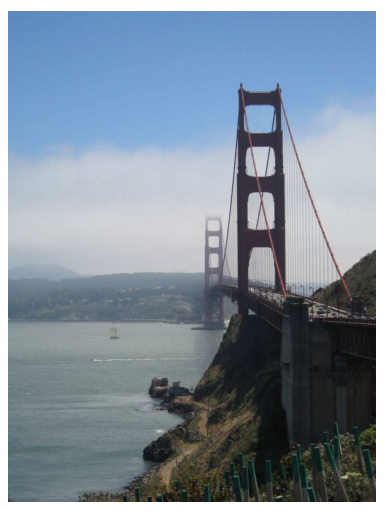
\includegraphics[scale=0.50]{Images/ea_photo_ama}}               
 \subfloat[Photo d'un Professionnel]{\label{fig:photopro}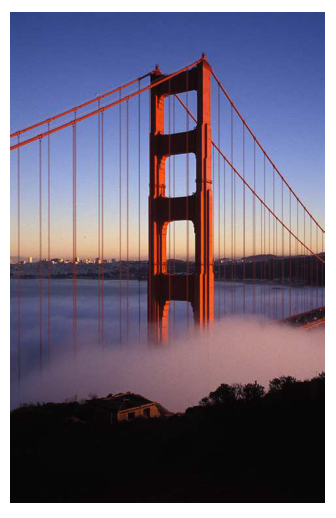
\includegraphics[scale=0.50]{Images/ea_photo_pro}}
 \caption{Comparaison entre la photo d'un amateur et celle d'un professionnel \cite{Ke}}
 \label{fig:ComparaisonPhotosAmateurPro}
\end{figure*}
\paragraph*{}
\label{crit:both}
De leur côté, Ke et al. \cite{Ke} confortent cette idée et ajoutent une liste d’autres critères de haut niveau qui permettent de déterminer le professionnalisme de celui qui l’a prise. Il y a tout d’abord la simplicité, c'est à dire à quel point il est facile de détacher le sujet du fond. Plus c'est simple, plus la photo est de bonne qualité. Cela se caractérise en pratique par la distribution des couleurs (ou le nombre de teintes): moins la palette utilisée est large, plus la photo est professionnelle; mais également le niveau de flou: plus une photo est floue, moins le soin apporté lors de la prise est grand et donc moins bonne est la qualité.
Vient ensuite le réalisme, c'est-à-dire à quel point la photo peut sembler atypique par rapport aux autres, c'est la petite touche qui la rend différente.
\paragraph*{}
Au final, certains articles comme celui de Ke et al. tendent à montrer que l'usage exclusif de l'une ou l'autre des catégories de critères n’est pas une solution en soit et que l’utilisation combinée des critères de haut et de bas niveau est nécessaire afin d’obtenir un résultat optimal. Si l’on se base uniquement sur les critères de bas niveau, on disposera de toutes les informations que l’on souhaite sur sa composition technique (histogrammes, palettes de couleurs, etc.) mais on n’aura pas d’indicateurs pour évaluer sa beauté conceptuelle. Avec les critères de haut niveau, on obtiendra de bien meilleurs résultats, on aura plus d’informations sur la composition de la photo (placement des personnes, des objets par exemple) mais cela restera quand même insuffisant. En effet, nous n’aurons pas les informations techniques comme la distribution des couleurs, la luminosité, etc, autant de critères qui servent à détecter la touche d’originalité d’un professionnel (voir point précédent~\ref{originalite}).

Ainsi, au final, c’est la combinaison des deux niveaux de critères qui permet de détecter correctement le degré de beauté d’une photographie.
Nous allons donc maintenant vous présenter de manière plus détaillée la liste des critères de chaque niveau mis en avant dans nos lectures :
\paragraph{Critères dits de haut niveau} : Ce sont dans l'ensemble des caractéristiques plus subjectives et que l'on peut calculer à partir de mesures faites à plus bas niveau. Cependant, une grande partie des critères haut niveaux tel l’originalité par exemple ne possèdent pas de consensus au niveau de leur définition, il n’est donc pas possible de les évaluer automatiquement. Nous allons vous présenter une liste de ceux pour qui il est possible de le faire aujourd'hui. Cette liste est divisée en trois groupes: le premier traite des critères liés à la composition structurelle des photographies, le second expose les critères relatifs au contenu, quant au troisième groupe, il s'agit des critères ne relevant pas des deux premiers groupes.\footnote{Les équation utilisées pour mesurer les critères s'exécutent dans le contexte suivant : la photographie en RGB doit être convertie dans l'espace HSV. Plusieurs matrices de deux dimensions $X x Y$ sont générées $I_H$, $I_S$ et $I_v$.}

\subparagraph{Attributs liés à la composition des photographies}
Sous cette étiquette sont regroupés les attributs caractérisant la manière dont sont composées les photographies. 
\begin{description}
\item[Règle des tiers]
Elle consiste à diviser la photo en blocs égaux en ajoutant deux lignes virtuelles verticales et deux lignes virtuelles horizontales. Il a  été "prouvé" qu’une photo est plus esthétique si le sujet se trouve sur l’une de ces lignes ou à l’une des intersections de ces lignes. Pour savoir si la photo respecte cette règle, on détecte le sujet principal de l’image et on calcule la distance entre le centre de la forme détectée et ces lignes ou intersections. Une autre méthode de calcul est basée sur le fait que l'objet principal est placé à la périphérie où à l'intérieur du rectangle intérieur. On y étudie la teinte moyenne dans l'espace HSV \footnote{HSV: désigne un espace colorimétrique dont les initiales signifient Hue, Saturation, Value. En français cela correspond à TSV (Teinte, Saturation, Valeur).} selon l'équation ~\ref{teintemoyenne}. 

\begin{equation}
teinteMoyenne = \frac{9}{XY}\cdot \sum_{x=\frac{X}{3}}^{\frac{2X}{3}} \sum_{y=\frac{Y}{3}}^{\frac{2Y}{3}} I_H(x,y)
\label{teintemoyenne}
\end{equation}

\item[Profondeur de champ]
La profondeur de champ désigne une technique où les objets ou personnes proches sont mises en avant sur la photographie par rapport au fond. Pour cela, on applique un flou sur  le fond, ce qui a pour effet de faire ressortir les objets non floutés (donc nets) et de donner une impression de profondeur à la photo. Zhuo et Sim \cite{Zhuo2011} présentent une méthode d’estimation de la défocalisation du sujet du fond dans une seule image. Pour cela, ils appliquent un flou gaussien sur l’image en  entrée. Un ratio entre l’image originale et l’image modifiée est calculé. Les auteurs ont montré que le flou sur les bords était lié à ce ratio. Ensuite est résolu un problème d’optimisation qui permet d’obtenir une carte de défocalisation. Leur méthode peut aussi être utilisée pour classer les pixels de l’image comme flou ou net.
\item[Couleurs complémentaires]
Il existe certaines couleurs qui vont mieux ensembles que d’autres, voire qui donnent une ambiance à la scène. Il s’agit des couleurs qui se trouvent à deux extrémités différentes du spectre de couleur. On va donc privilégier ces complémentarités de couleurs dans une photographie afin de la rendre plus belle à regarder ou lui donner un certain effet de style. Pour détecter cela, une solution est de construire un tableau  qui indique dans quelle partie du spectre se trouve une couleur puis d’apprendre au logiciel laquelle se retrouve fréquemment  avec quelle autre via un algorithme d’apprentissage.
\item[Présence d'un objet saillant]
Cet indicateur permet de détecter les objets larges séparés du fond de l’image. Pour cela, trois techniques sont combinées : une carte de contraste multi-échelle pour détecter les formes, un histogramme des pixels avoisinants pour détecter les changements de couleur et dans le même ordre d’idées une cartographie de la distribution des couleurs de l’image.
\end{description}
\subparagraph{Attributs liés au contenu}
Les attributs liées au contenu sont axés sur ce qui a été pris en photographie. Il s'agit donc de critères explicitant le sujet et son environnement.
\begin{description}
\item[Présence de personnages humains]
C’est un attribut de haut niveau qui permet d’indiquer si des personnes sont présentes ou non sur une image. Les études indiquent que les observateurs humains apprécient les photos mettant en scène leurs congénères. Pour cela, on se sert d’algorithmes automatiques comme celui développé par Viola et Jones \cite{Viola2004}. La limite de ce critère est que le performance dépend de l’algorithme utilisé et généralement de l’apprentissage réalisé au préalable.
\item[Portrait d'une personne]
Un portrait est aussi un type de scène que l’on apprécie. L’indice de détection de portrait consiste à indiquer si les pixels représentant le visage sur la photographie représentent plus d’un certain pourcentage de l’image et si cette dernière peut donc être classifiée comme portrait. Il s’agit d’un simple seuil à dépasser, par exemple si le visage représente plus de 25 \% de l’image.
\item[Photo en intérieur ou extérieur]
Ce paramètre indique si la photo a été prise en intérieur ou en extérieur. Pour cela, on utilise un algorithme avec apprentissage sur un jeu de données spécifiques contenant les deux types de scènes. Ce paramètre permettra de juger la beauté de la photo sur le principe qu’une photographie en extérieur est plus esthétique qu’une photographie en intérieur (on parle ici de la photographie en général et non du cas particulier du portrait). Ce critère seul est assez compliqué à utiliser pour discriminer l’esthétique, il gagne à être combiner avec d’autres.
\item[Type de scène]
L’indicateur type de scène permet de détecter l’environnement dans laquelle la photographie a été prise, s’il s’agit d’un salon, d’un bureau, d’une plage \ldots Pour cela on s’appuie sur un algorithme de détection du type SVM\footnote{SVM: en anglais Support Vector Machine et en français Machine à Vecteurs de Support. Les SVM sont des classifieurs basés sur des techniques d'apprentissage supervisé.} ayant eu une phase d’apprentissage au préalable.
\end{description}

\subparagraph{Autres attributs}
Cette catégorie regroupe les attributs hors des deux premières catégories.
\begin{description}

\item[Luminosité du ciel]
La luminosité du ciel va jouer un rôle important. En effet, cela va apporter un éclairage différent sur la scène et donc une ambiance particulière. Le fait que la photographie soit prise de jour ou à la tombée de la nuit ne va pas apporter la même atmosphère. De la même manière, une photo prise par beau temps va être jugée plus jolie qu’une photo prise par temps gris. La première étape ici est de détecter la partie relative au ciel dans la photo, puis d’analyser l’histogramme des couleurs et/ou la luminosité.
\item[Mesure du caractère familier]
L’être humain compare instinctivement une photo qu’il regarde avec celles qu’il a déjà vues dans le passé. Ainsi, quelque chose de "nouveau" pourra avoir un certain impact sur l’observateur. Pour déterminer ce facteur de manière informatique, on calcule la distance de certains critères de bas niveau de l’image par rapport à ces critères obtenus en apprentissage sur d’autres photos. Ce critère est difficilement utilisable quand on analyse une photographie seule (et non par lots).
\item[Étude de la texture]
Le fait que l’image soit lisse ou granuleuse va avoir un impact sur l’évaluation de sa beauté. Une image granuleuse sera plutôt bien évaluée tandis qu’une image lisse aura plutôt tendance à indiquer un hors champ et donc une image de mauvaise qualité. Pour détecter cela, on applique des filtres de texture pour détecter si l’image est granuleuse ou lisse.
\item[Taille et ratios]
La taille d’une image et surtout le ratio hauteur par largeur aura un gros impact sur la perception de l’utilisateur humain. Pour détecter cela, on introduit une simple formule d’échelle pour détecter si l’image respecte l’une des normes photographiques. Certains préfèrent les rations 4 :3 ou d’autres 16 :9. Un indicateur pour la taille est $taille = X+Y$ (somme de la hauteur et de largeur de l'image) et pour le ratio on a $ratio = \frac{X}{Y}$.
\item[Complexité des formes]
Il a été prouvé que les formes avaient un impact sur la perception de l’observateur, l'idée étant de détecter par un traitement automatique quelles formes plaisent plus que d’autres. Cependant, il s’agit d’un travail laborieux car il faut mettre en place un outil pour détecter tous les types de formes et ensuite lui faire apprendre sur une base d’images quelles formes ont une réelle signification et dans quel contexte.
\item[Image colorée \& nombre de couleurs]
L’étude des couleurs dans une image permet d’évaluer plusieurs choses. Tout d’abord, cela permet de déterminer si l’image est monochromatique  ou polychromatique. S’il n’est pas sensé y avoir un effet particulier sur la photo (comme un filtre de type sépia par exemple) alors on peut déduire qu’il y a eu un problème au niveau de la prise. Ces images seront alors considérées comme prises par un amateur.

Le deuxième point pour séparer une photo prise par un amateur de celle prise par un professionnel, est que la seconde possède moins de couleurs distinctes. En effet le photographe va jouer sur les couleurs complémentaires pour mettre en valeur le sujet avec peu de couleurs. Il utilisera quand même des filtres pour jouer sur les nuances. En conclusion, on trouvera donc moins de couleurs différentes mais plus de nuances d’une même couleur au niveau du sujet sur une photo professionnelle. À l’inverse, au niveau du fond de l’image on trouvera peu de nuances étant donné que c’est le sujet qui doit être mis en avant.

Dans le cas d'image en niveaux de gris, on ne compte qu'une couleur. Sinon, on convertit l'image colorée dans le domaine HSV. Un histogramme $H$ de 20 classes représentant les pixels de couleur significative (ayant une luminance dans l'intervalle [0.15,0.95] et une saturation $s > 0.2$). Avec $m$ la valeur maximale de l'histogramme on estime un nombre $N$ de couleurs les plus présentes: 
\begin{equation}
N = \left\{i|H(i)>\alpha \cdot m\right\}
\end{equation}
Avec un $\alpha$ valué à 0,05, il semble que Ke et al. \cite{Ke} obtiennent de bons résultats. La qualité de l'image exprimée en nombre de couleurs peut être calculée avec l'équation ~\ref{nombreteintes}. Dans l'ensemble, une image qui contient peu de couleurs est plus maîtrisée et est donc plus proche d'un rendu professionnel. 
\begin{equation}
q_h = 20 - ||N||
\label{nombreteintes}
\end{equation}


\end{description}

\paragraph{Critères dits de bas niveau} : Ils relèvent directement des caractéristiques objectives déterminées à partir des métadonnées des photographies. Contrairement aux critères de haut niveau, ils sont tous calculables car basés sur les propriétés physiques de la photographie.
\subparagraph{Histogramme de la couleur du ciel}
Pour évaluer les critères de haut niveau relatifs aux type du ciel que nous avons présentés précédemment, il est nécessaire de pouvoir se baser sur des critères de bas niveau. Le critère retenu est un histogramme dans l’espace HSV pour déterminer la tendance dominante. L’histogramme peut être utilisé à plus haut niveau pour différencier les différents types de ciel.
\subparagraph{Propriétés de Haar}
Les propriétés de Haar relèvent d’une technique de détection des sous-régions d’une image. Ces propriétés sont directement utilisées par l’algorithme de détection des visages élaboré par Viola et Jones \cite{Viola2004}. Par exemple, si la zone des yeux est plus sombre que celle des joues, ces zones peuvent être modélisées par des rectangles adjacents. La position de ces rectangles devient de plus en plus précise en ayant une grande base d’apprentissage. La méthode de Viola et Jones utilise des fenêtres sur une image pour séparer les régions et déterminer une boîte englobant un visage s’il y en a.
\subparagraph{Mesure du flou}
Pour mesurer seulement le flou, on peut appliquer un filtre gaussien pour retirer les hautes fréquences de l’image puis une transformée de Fourier. Ke et al. \cite{Ke} procèdent de cette manière : 

Une photographie floue est définie comme la convolution d'une image nette $I_s$ par un filtre lissant Gaussien $G_\sigma$:
\begin{equation}
I_b = G_\sigma * I_s 
\end{equation}
Ensuite, pour déterminer la fréquence maximale de l'image floue, on utilise sa transformée de Fourier pour pouvoir compter les fréquences dont l'amplitude est supérieure à un seuil $\theta$.
\begin{equation}
F = FFT(I_b)
\end{equation}

\begin{equation}
C = \left\{(u,v) | |F(u,v)| > \theta\right\}
\end{equation}
 
Le filtre gaussien supprimant les hautes fréquences, la fréquence la plus haute est $||C||$. Ke et al. \cite{Ke} définissent de cela que la qualité de l'image est: 
\begin{equation}
q_f = \frac{||C||}{||I_v||} \approx \frac{1}{\sigma}
\end{equation}
où le paramètre $||I_b||$ est la taille de l'image. Avec un $\theta = 5$, ils ont calculé avec un classifieur que la qualité de l'image d'un professionnel était d'environ 0,91 et que celle d'un amateur était de 0,58.

Le niveau de flou de la photo est inversement proportionnel à l’indice $\sigma$ obtenu. Pour la profondeur de champ qui est un critère de plus haut niveau une méthode a été expliquée précédemment.

\subparagraph{Carte de contraste multi-échelle}
Cette technique bas niveau identifie des zones de pixels au contraste similaire dans une image. L’image est analysée à plusieurs échelles, à un niveau local et global. Une carte des régions de contraste est réalisée sur les objets et formes qui y sont détectés. Cette carte peut être utilisée à un plus haut niveau pour comparer une région à une carte de contraste d’un objet connu. Avec cela on peut déterminer ce qui se trouve sur une image, le tout à condition que la base de connaissances soit suffisamment fournie. Cet outil est difficilement applicable dans un premier temps car il présuppose une détection de formes ou d’objets dans l’image traitée.
\subparagraph{Saturation et teinte}
Une photographie est composée de tout un ensemble de pixels possédant chacun une teinte d’une intensité plus au moins forte. Si l’intensité d’une couleur est forte on parle de haute saturation et la couleur est alors vive. À l’inverse une saturation faible donne une impression de couleur terne. En utilisant ce critère on peut à un niveau local ou global étudier les conditions de prise de photographie par exemple. Une saturation globale très faible juge une image fade. Pour obtenir un indicateur sur la saturation on peut utiliser dans l'espace HSV : 
\begin{equation}
saturationMoyenne = \frac{1}{XY}\cdot \sum_{x=0}^{X-1} \sum_{y=0}^{Y-1} I_S(x,y)  
\end{equation}

\subparagraph{Luminosité}
La luminosité est l’un des critères de base de la photographie. Une surexposition  comme une sous-exposition conduiront à une image trop claire ou trop sombre et elles seront donc évaluées négativement. On reconnaîtra donc une image de qualité professionnelle comme une photographie de luminosité moyenne correspondant à la lumière du jour. Pour déterminer si notre photo correspond ou non, on fait la moyenne de l’intensité des pixels et on compare la valeur obtenue avec celle attribuée à une bonne exposition.
\subparagraph{}
Tous ces critères nous permettent de juger les photographies de manière générale, mais n'existent-ils pas des propriétés propres au cas des photographies de portrait ? C'est ce que nous allons étudier dans le prochain point.
\subsection{L’art d’un portrait réussi}
Maintenant, concentrons-nous sur le caractère différent des photographies de portrait et sur ce qui est utilisé pour différencier les bonnes des mauvaises.
Prendre une photographie de portrait est une activité qui s'est beaucoup démocratisée avec l'avènement des appareils photos numériques et des téléphones intelligents aux capteurs de plus en plus puissants. Malgré les scènes de prises de photos dédiées aux photos de portrait, les résultats ne nous satisfont pas toujours.
\paragraph*{}
Très souvent, affligés de ce constat, nombreux sont ceux qui se tournent vers la retouche de leurs clichés. Les principaux points retouchés dans les photographies de portrait sont: la netteté du visage, le retrait des yeux rouges (dû à l'usage du flash), un équilibrage de la balance des blancs afin de redonner à la peau une teinte plus naturelle, la correction des imperfections cutanées, la modification de la forme de certaines zones du visage (comme le nez), la diminution des rides et signes de l'âge... Ce panel n'est pas exhaustif étant donné que selon les photos, la correction de certains points est plus utile que sur d'autres.
\paragraph*{}
La retouche peut s'avérer coûteuse, surtout en ce qui concerne l'acquisition d'outils performants. Une autre alternative est possible pour ceux n'ayant pas de réticence pécuniaire, à déléguer ces opérations à un professionnel (dont le coût pourrait être inférieur). Les chercheurs se sont aussi intéressés à nos visages et à ce qui nous plaisait, cela pour être en mesure d'évaluer les clichés. L’apparence de la peau (peau lisse) est une préoccupation majeure des personnes qui cherchent à supprimer les imperfections comme le montrent Konoplev et Alexey \cite{Konoplev2012} ainsi que Ciuc et al. \cite{Ciuc2010}. Les deux articles mettent au cœur de leur traitement d'amélioration la peau puisqu'elle est supposée dans une photographie de portrait avoir une occupation de l'espace importante.
\paragraph*{}
Nous ne nous intéresseront pas dans ce projet à ce qui définit la beauté intrinsèque des visages que l'on a photographiés, mais nous pouvons citer l'étude suivante, par Leyvand et al. \cite{Leyvand2008}, qui a cherchée à déterminer ce qui fait qu'un visage est attirant ou non. Dans leurs travaux, à l'issue de l'analyse d'une base d'images ayant des niveaux d'attirance différents,  une méthode a été développée pour modifier des visages de sorte qu'ils nous plaisent plus. Cette technique est basée sur la construction de masque de visages de beauté moyenne. L'intérêt de cette étude est que nous serions sensibles à un certain type de visage mais aussi d'expression.
\paragraph*{}
De plus, les êtres humains sont très sensibles à la symétrie des visages comme le présente Perret et al. \cite{Perrett1999}. Même si nous préférons des visages symétriques, leur article indique qu'un certain degré d'asymétrie est quand même appréciable et plus attirant. La figure~\ref{fig:VisagesSymetriques} présente en haut les visages naturels et en-dessous une version corrigée de la symétrie des visages. On peut constater que l'on préfère majoritairement les secondes versions avec une symétrie corrigée.
\begin{figure*}
	\centering
	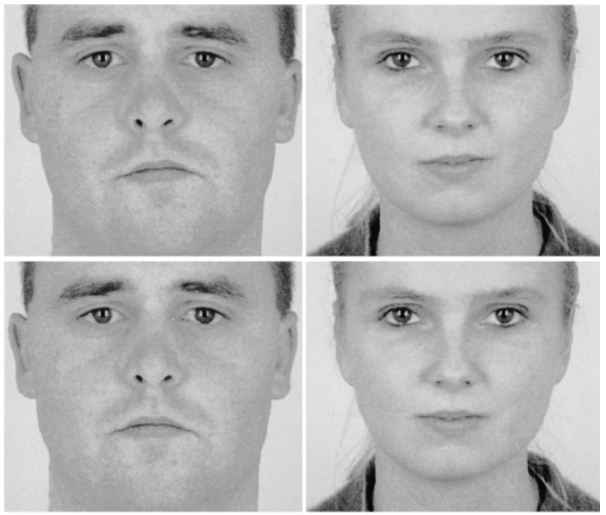
\includegraphics[width=0.5\textwidth]{Images/ea_visages_symetriques}
	\caption{Comparaison entre des visages asymétriques et plus symétriques \cite{Perrett1999}}
	\label{fig:VisagesSymetriques}
\end{figure*}
Males et al. \cite{Males2013} ont développé une procédure d'évaluation de photographie de portraits sur 10 critères. Certains sont communs aux photographies classiques comme la profondeur de champ et la luminosité, et certains sont spécifiques au cas des portraits tels que la netteté du visage et la taille du visage. Les critères qui ont été retenus sont les suivants :
\subparagraph{Critères vus précédemment} profondeur de champ, contraste, composition (type règle des tiers)
\subparagraph{Netteté} Dans ce type de photo, c'est bien entendu le visage qui doit être net. Un visage flou n'est pas agréable à regarder. Son calcul est basé sur deux facteurs (mesure spectrale sur l’ampleur de spectre local et une mesure spatiale sur la variation des maximums locaux). Cependant ce critère est moins apprécié sur certaines zones du visage comme les rides par exemple.
\subparagraph{La clarté} Dans le sens d'une image peu chargée et claire. Le sujet doit être illuminé de manière homogène et l’image devrait contenir peu d’ombre. L’éclairage sur le visage est ainsi important et pour évaluer sa qualité, une moyenne des pixels de la luminance dans la boite englobant le visage doit être calculée. C’est dans l’espace HSL\footnote{HSL: désigne un espace colorimétrique dont le nom signifie en anglais Hue Saturation Lightness, et en français Teinte Saturation Luminance.} qu’est effectué ce calcul (la composante L correspondant à la luminance).
\subparagraph{Coupure et la surexposition} Un visage surexposé à la lumière donne une impression de photographie mal pensée. Le degré de  surexposition est calculé dans l’espace de gris de la photo. La surexposition est estimée comme le pourcentage de la zone du visage qui a ses pixels valués à la plus forte intensité (les plus clairs).
\subparagraph{Taille du visage} C'est un critère relatif à l’essence des photos de portrait. C'est un critère qui fait écho à celui de la présence d'un objet saillant et donc primordial. L’œil doit être attiré par le visage, il faut donc évaluer un ratio entre la zone du visage et la taille de l’image totale.
\subparagraph*{}
Une photo comme la figure~\ref{fig:VisageAgreable} est un bon exemple du respect de ces critères.
\begin{figure*}
	\centering
	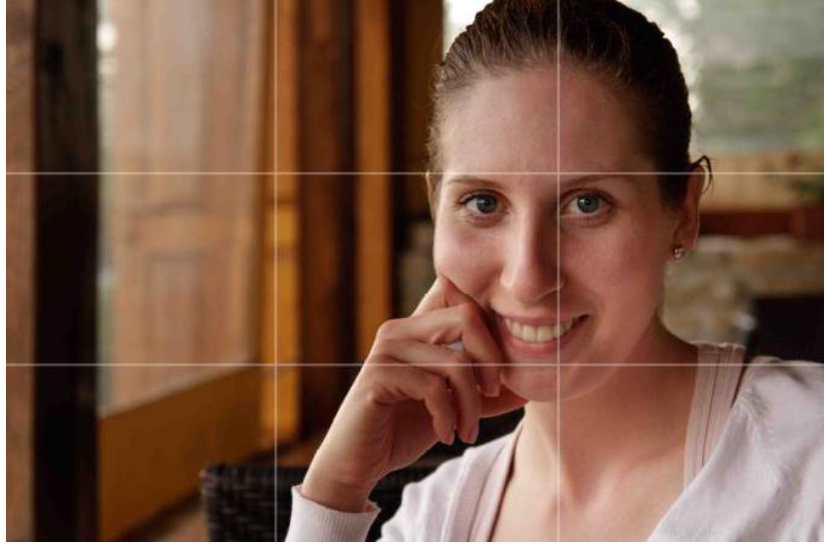
\includegraphics[width=0.7\textwidth]{Images/ea_visageagreable}
	\caption{Une photographie respectant les critères esthétiques dans le cas de portrait \cite{Males2013}}
	\label{fig:VisageAgreable}
\end{figure*}
Nous connaissons désormais les grands critères utilisés pour analyser les photographies ainsi que ceux relevant spécifiquement des portraits. Dans le prochain point nous allons parcourir quelques idées pour l'évaluation de la qualité des images.
\subsection{Techniques d’évaluations et bases d’images}
\label{part:PointEvaluation}
Cette partie s’inscrit dans le processus de discrimination des photographies et présente brièvement quelques travaux qui ont été menés pour évaluer la qualité de photographies. L’évaluation de la qualité des photographies que nous générerions avec la méthode que nous proposons serait intéressante. Si le temps nous le permet cet aspect pourrait être vu plus en détails à la fin du projet.
\paragraph*{}
De nombreuses techniques utilisent des classifieurs basés sur un apprentissage supervisé, comme celle de Males et al. \cite{Males2013}. Dans leur méthode, les critères de bas niveau sont calculés sur l’ensemble de l’image tels que le contraste et le nombre de teintes. Les critères de haut niveau sont directement calculés dans la boîte englobant le visage (détecté par la méthode de Viola et Jones \cite{Viola2004}). Une fois tous les critères calculés, ils sont normalisés et inclus dans un vecteur. Les vecteurs obtenus sur plusieurs images vont alimenter les classifieurs. Deux classifieurs ont été utilisés dans leurs travaux afin de comparer leurs performances, il s’agit de SVM et d’AdaBoost. SVM a été en moyenne meilleur qu’AdaBoost\footnote{AdaBoost: raccourci du nom Adaptive Boosting. Il s'agit d'une méthode d'apprentissage automatique.}. Ils ont établi un comparatif de la précision des deux classifieurs dans le tableau~\ref{tab:ComparaisonSVMAdaBoost}. On peut constater que l'usage d'un SVM semble un peu plus performant.
\begin{table}
\begin{center}
\begin{tabular}{|c|c|}
\hline
& Précision de la classification \\
\hline
SVM & 86.33\% \\
\hline
Real AdaBoost & 84.66\% \\
\hline
\end{tabular}
\end{center}
\caption{Tableau des résultats de classification avec des techniques différentes \cite{Males2013}}
\label{tab:ComparaisonSVMAdaBoost}
\end{table}
\paragraph*{}
Afin que ces méthodes fonctionnent, il faut être en mesure de fournir une base de visages qui permettraient d'entraîner les algorithmes mais aussi de les éprouver en phase de test.
Des bases avec de grands nombres de photographies de portrait sont indéniablement préférables. Le site du Laboratoire d'Informatique et des Systèmes Adaptatifs (LISA) de l'université de Montréal, liste des bases d'images qui pourraient être utilisées par ses étudiants\footnote{\url{http://www.iro.umontreal.ca/~lisa/twiki/bin/view.cgi/Public/FacesDatabases}}. Cependant toutes les bases ne sont plus accessibles, et pour celles qui le sont, des demandes d'utilisations doivent être envoyées aux laboratoires de recherche responsables de ces bases. Dans la majeure partie de leurs bases, de nombreuses expressions de visages sont enregistrées et peuvent être utilisées pour tester la robustesse des algorithmes de détection des visages et des zones caractéristiques comme les yeux, le nez, la bouche.

Nos recherches nous ont conduites à un rapport de projet de recherche écrit par Charlène David et Mariam-Kaou Sissoko\footnote{\url{http://madoc.univ-nantes.fr/pluginfile.php/480996/mod_folder/content/3/DAVID\%20SISSOKO\%20Rapport\%20v2.pdf?forcedownload=1}}. Leur étude était axée sur la beauté des visages, et afin d'éprouver leur proposition d'extraction et de notation des visages, elles ont utilisé les bases d'images de Karolinska et de LEI.

La base Karolinska répertorie des visages sous différentes expressions de suédois. Ce sont donc des photographies de visages européens. Cette base propose une base d'images de résolutions convenables (562x762) en comparaison de résolutions plus faibles dans la base FEI de 260x360. Par contre la base FEI met en avant 200 visages de brésiliens sous plusieurs positions différentes. La base de Karolinska est donc plus qualitative que la base FEI, mais on observe l'inverse en ce qui concerne la partie quantitative. Le point qui pourrait au final nous faire pencher vers la base FEI, est la présence d'un fond qui n'est pas terne comme dans la base Karolinska.
\paragraph*{}
À présent que nous savons ce qu'il faut étudier sur une photographie de portrait, il est temps de nous intéresser aux méthodes existantes qui permettent d'améliorer et d’en retoucher une de manière automatique. Puis nous nous forgerons un comparatif des critères esthétiques importants et des méthodes qui seront présentées.

\section{\ldots aux techniques d’amélioration automatiques de nos photographies de portrait}
L’étude des critères esthétiques faite, nous savons quels sont les éléments pertinents qui influent dans la qualité des photographies de portrait. Cette seconde partie de l’état de l’art présente une analyse critique des méthodes et techniques existantes qui ont été développées en vue d’améliorer nos clichés et de faire ressortir tout leur potentiel
Cette section débute par la présentation des techniques de correction dans un esprit global, elle sera suivie logiquement par celles ayant une essence locale.
\subsection{Technique globale pour l’amélioration de la peau}
Nous allons commencer par vous présenter les traitements qui agissent de manière globale sur une photographie de portrait. Le premier, inventé par Lee et al. \cite{Lee} traite de l'amélioration de portraits numériques via un adoucissement de la peau.
\paragraph{Présentation}
Cet article s'inscrit dans le mouvement des techniques d'amélioration de portraits numériques.
Plus particulièrement, il présente un algorithme réalisant une amélioration de la peau automatique qui est aussi illustré par la figure~\ref{fig:FonctionnementLee}.

Plusieurs étapes sont nécessaires pour réaliser ce traitement, à commencer par une phase de localisation des visages contenus dans la photographie en utilisant la méthode de Viola et Jones \cite{Viola2004}.
Tous les points d'intérêts sont d'abord enregistrés comme le nez, la bouche, les yeux.
Ensuite intervient une phase d'adoucissement de la peau.
Dans cette phase il faut créer un masque de pixels qui relèvent de la peau ou non.
Un GMM (Gaussian Mixture Model pour Mélange de Modèles Gaussiens) est utilisé afin de déterminer des masques de pixels correspondant à la peau ou non.
Sur l’image originale est appliqué un flou gaussien. À partir de cette version floue, on récupère seulement les pixels situés dans le masque de peau. On superpose ensuite le masque de peau original avec sa version floue (avec une opacité à 50 \%) afin d’obtenir un visage plus lisse. Le fond, et les zones ne relevant pas de la peau tels les yeux ne sont pas modifiés.

Les résultats de ce traitement sont revendiqués comme aussi réussis que ceux obtenus de manière manuelle avec des outils de retouche d'images.
\begin{figure*}
	\centering
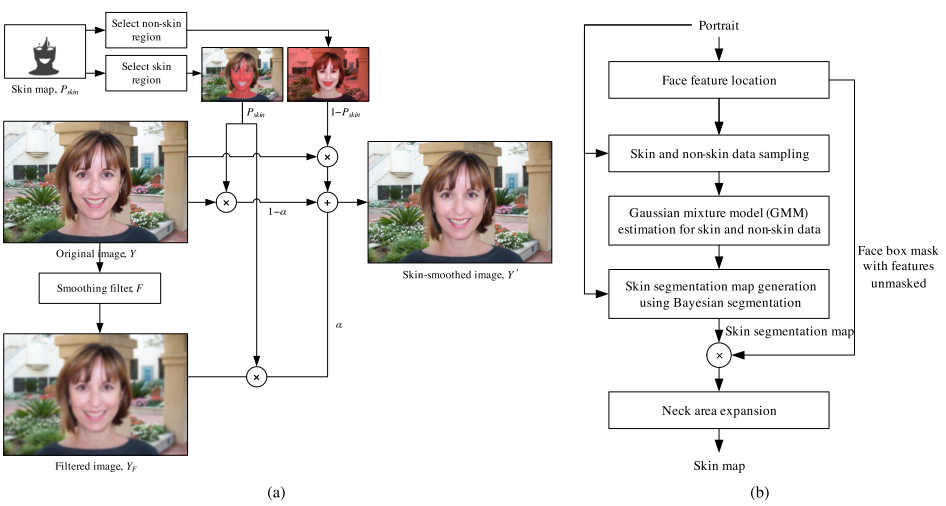
\includegraphics[width=0.9\textwidth]{Images/ea_algo_smoothing}
	\caption{Principe de fonctionnement de la méthode développée par Lee et al. \cite{Lee}}
	\label{fig:FonctionnementLee}
\end{figure*}
\paragraph{Analyse}
Dans l'esprit des traitements manuels et semi-automatiques, cet algorithme automatique permet, en tout cas d'après les photos jointes à l'article, de constater un résultat similaire.
Les grandes étapes de l'algorithme sont communes à d'autres techniques d'imagerie, comme l'acquisition et le repérage des points d'intérêts.
Ce traitement du visage couvre une partie des améliorations possibles d'une photo de portrait. Cet article se concentre exclusivement sur le traitement de la peau, qui induit une correction par application de flou des rides par exemple.
\paragraph{Intérêt pour notre sujet}
On gagne en temps de détection, on n’a pas besoin de localiser et d’isoler chaque petite imperfection, on récupère la totalité du visage et on corrige l’ensemble des pixels de peau. En comparaison avec d’autres techniques, de bons résultats sont obtenus avec une méthode qui a une complexité qui dépend majoritairement de la détection des bons pixels de peau.
\paragraph{Limites}
Cette technique applique de manière générale un flou sur la peau. Ce flou peut induire une perte de détails et de la netteté du visage. Or, il ne faudrait pas que la profondeur de champ s’amenuise à cause d’une augmentation du flou sur l'objet saillant de la photographie. Cette technique, à un moment donné, utilise un flou gaussien sur l’image intégrale, il est dommage que le fond flou ne soit pas réinjecté dans l’image résultat pour augmenter la profondeur de champ.

Cette première méthode a l’avantage d’être assez simple à appliquer dès lors que la détection de la peau est précise. Le fait d’appliquer un flou sur le visage, provoque un lissage de ce dernier, une réduction des rides, etc. , donc d’imperfections cutanées. Cette méthode permet aussi de traiter la peau des sujets portant une barbe ou des lunettes par exemple.
\subsection{Méthode d’amélioration globale de portrait par déformation du visage}
Nous allons à présent nous intéresser au cas d’une nouvelle méthode d’amélioration de visages en les déformant.
\paragraph{Présentation}
Dans leur article, Leyvand et al. \cite{Leyvand2008} traitent d'un procédé intéressant pour améliorer un portrait en utilisant la technique de déformation du visage pour le faire ressembler à un visage jugé plus beau. La figure~\ref{fig:FonctionnemenLeyvand} illustre le fonctionnement de leur méthode. Leur méthode fonctionne de la manière suivante:
\begin{enumerate}
\item La première étape consiste à détecter le visage dans la photographie ainsi que ses éléments caractéristiques. Les points repérés vont être combinés afin d’obtenir une carte du visage.
\item Cet ensemble de points est alors transformé en graphe où le poids de chaque arc est la distance entre les deux nœuds (sommets équivalents aux points caractéristiques du visage). Ce graphe de distances est calculé en utilisant la triangulation de Delaunay.
\item L'algorithme possède une base de distances acquises par apprentissage sur des photos évaluées comme belles par des utilisateurs. Ainsi lors de la troisième étape, l'algorithme va détecter la photographie la plus jolie dans un intervalle de distances proches et retourner ces distances.
\item Le but est de rester dans un intervalle proche est de ne pas trop modifier l'image d'origine et de rester fidèle à l'apparence originelle de la personne.
Lors de la quatrième étape, le logiciel va déplacer les pixels du visage par déformation de manière à ce qu'ils cadrent avec le masque de distances du visage modifié à l’issue de l'étape précédent.
\end{enumerate}
\begin{figure*}
	\centering
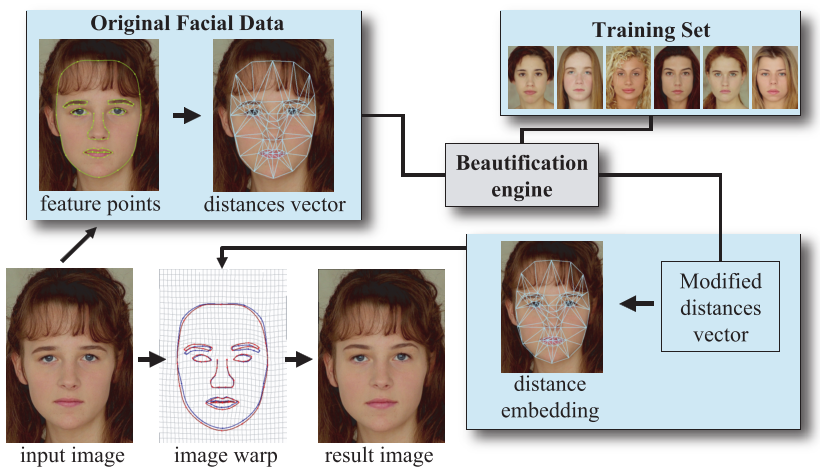
\includegraphics[width=0.8\textwidth]{Images/ea_algo_datadriven}
	\caption{Principe de fonctionnement de la méthode développée par Leyvand et al. \cite{Leyvand2008}}
	\label{fig:FonctionnemenLeyvand}
\end{figure*}

\paragraph{Analyse}
Les résultats fournis dans l’article semblent encourageants et constituent une alternative viable à l’amélioration de portrait. L’obtention de bons résultats dépend fortement de la pertinence et la taille de la base des photographies pour l’apprentissage.
\paragraph{Intérêt pour notre sujet}
Cet article nous a permis de voir les limites à partir desquelles on ne pouvait plus parler de la correction d’imperfections mais plutôt de modification du visage. Il présente une technique efficace pour réaliser des traitements d’améliorations dans le plan 2D.
\paragraph{Limites}
En utilisant cette technique, on peut facilement tomber dans la modification de la structure du visage. Il faut alors se poser la question suivante : à partir de quel seuil peut-on considérer que nous n’avons plus affaire au même visage ?
Cet article nous a présenté une méthode d’amélioration structurelle des visages. Elle est basée sur une base d’apprentissage utilisée par une machine à vecteurs de supports pour la régression (SVR\footnote{SVR: Sous catégorie de SVM dédiée à la regression. SVR signifie Support Vector Regression.}).
\subsection{Méthode d’amélioration des photos de portrait par enchainement de traitements sur différentes imperfections}
Nous passons à présent aux méthodes d’améliorations par traitements locaux. Dans ce premier article, écrit par Matraszek et Simon \cite{Matraszek2004}, on nous présente un algorithme utilisé par un logiciel breveté afin d'améliorer un portrait. Cet outil combine les améliorations sur plusieurs régions.
\paragraph{Présentation}
\subparagraph{}
Cet article nous présente un algorithme qui va détecter les zones du visage et permettre à l'utilisateur de les modifier manuellement (choisir la "dose de correction"). Ce logiciel est conçu pour être utilisé par un public non professionnel et est donc constitué de différentes jauges qui permettent d'augmenter ou de diminuer une valeur dans les zones ciblées. On dénombre quatre zones d'améliorations possibles : la peau, les yeux, les dents et la texture de la peau. Le fonctionnement général de leur outil est illustré avec le diagramme ~\ref{diag:diagrammebatch}.
\begin{figure*}
\centering
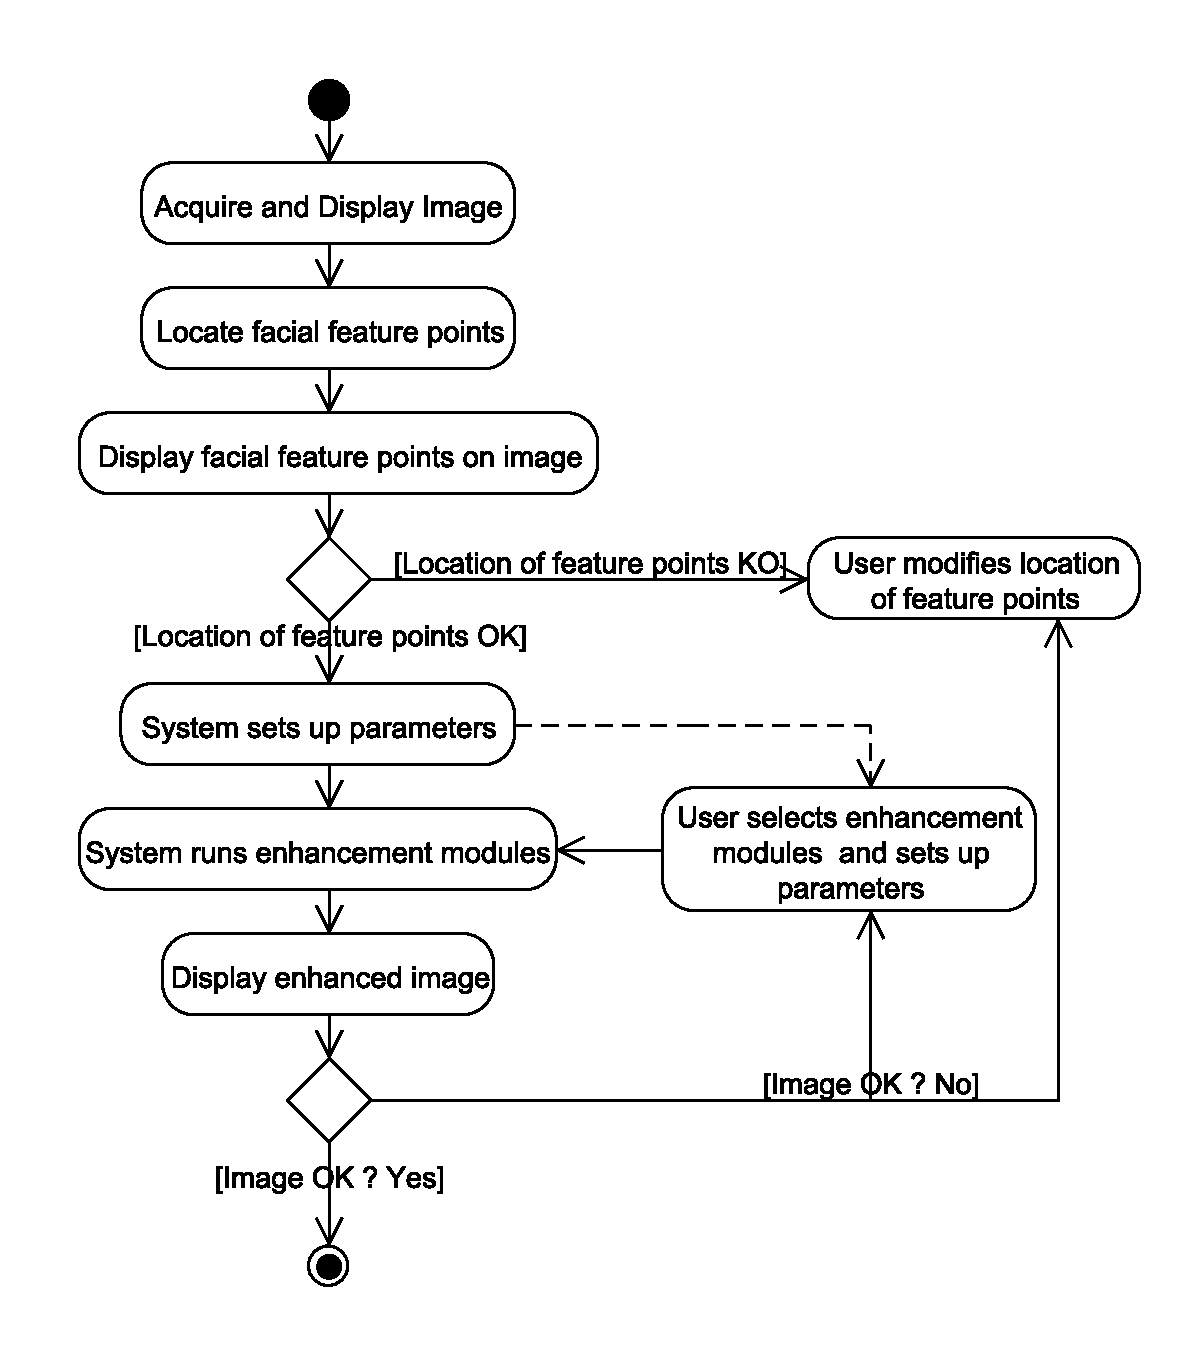
\includegraphics[height=9.5cm,width=7.5cm]{Images/ActivityBatch.eps}
\caption{Diagramme d'Activités correspondant à la méthode de Matraszek et Simon \cite{Matraszek2004} pour une image}
\label{diag:diagrammebatch}
\end{figure*}

\subparagraph{}
En ce qui concerne l’essence de l’algorithme, le traitement est effectué en plusieurs étapes : détection du ou des visages présents dans l’image traitée, extraire les zones clés de chaque visage comme la peau, les yeux, le nez, la bouche, les sourcils, le cou, les cheveux. Les visages sont donc segmentés selon toutes ces caractéristiques analysées. 

À la suite de cela, pour chaque partie du visage, il a été développé un traitement correctif. Les paramètres de ces traitements sont déterminés automatiquement au moyen d’algorithme permettant d’obtenir le genre et l’âge du visage traité (au moyen d’une méthode utilisant un SVM). Ils utilisent aussi une classification des pixels de peau afin d’inclure le cou.

Un utilisateur peut choisir d’appliquer dans l’ordre qu’il désire les différents traitements. Si ce n’est pas le cas, le logiciel dispose d’un ordre prédéfini: correction de la teinte de la peau, de la blancheur des dents et des yeux. Il termine par une modification de la structure du visage.
\subparagraph{}
Une amélioration des yeux citée pourrait être la correction de la balance des blancs et des couleurs de l’iris des yeux. Une présentation des principes des méthodes est réalisée dans la dernière partie de l’article.
\paragraph{Analyse}
Cet article nous permet de voir que des solutions payantes ont déjà été développées et nous donne une idée globale des améliorations réalisables. La solution proposée est donc un enchaînement d’améliorations donnant une image de meilleure qualité. Cet article présente les calculs pour la plupart des techniques d’améliorations. On note cependant, dans l'enchaînement, la présence d’un traitement de la texture de la peau qui altère la structure du visage. Si nous devions suivre le principe de la méthode présentée, nous ferions le choix de ne pas inclure ce dernier point.
\paragraph{Intérêt pour notre sujet}
On peut détecter chaque imperfection et lui appliquer un traitement différent selon sa nature. L’amélioration est déterminée pour la zone, on a donc plus de chance de gommer l’imperfection alors que le traitement global a tendance à améliorer le tout sans se préoccuper si l’imperfection locale a bien été gommée. Le plus de leur technique réside dans les multiples traitements réalisés. On peut choisir de privilégier une correction plus qu’une autre. De plus ces corrections pourraient être réutilisées séparément.
\paragraph{Limites}
On est obligé de détecter et traiter toutes les imperfections, ce qui est plus lourd en temps de traitement.
Il y a toujours un risque de récupérer le mauvais pixel représentatif et de l’étendre aux pixels voisins.
Comme pour l’article sur la déformation du visage, on modifie l’apparence originelle de la personne. Il faut donc se poser les mêmes questions sur l’éthique de cette pratique et si nous décidons de l’utiliser.
\subsection{Méthode d’amélioration des photos de portrait sur des sous-régions du visage}
Toujours dans le cadre des méthodes de corrections localisées, un nouveau traitement automatique du visage et de la peau est présenté dans l’article de Ciuc et Al. \cite{Ciuc2010}. Sa particularité est la limitation de la correction des visages dans des sous-régions de ce dernier.
\paragraph{Présentation}
La technique présente une amélioration de sous régions de l’image.  Elle repose sur une détection préalable des régions de la bouche et des yeux du visage. Les autres zones ne sont pas traitées.
L’image segmentée, une suppression du bruit peut être appliquée (même s’il est précisé qu’il vaut mieux s’en soucier lors de la prise de photo) ensuite c’est la luminance qui va être la cible d’améliorations. Si elle est trop faible on augmentera sa valeur, afin d’augmenter la blancheur du blanc des yeux et celle des dents. L’espace de couleur utilisé lors des améliorations est l’YUV\footnote{YUV: il s'agit d'un autre espace colorimétrique. Cet espace est divisé en trois composantes. Y correspond à la luminance et U/V correspondent à la chrominance.} pour la séparation luminance/chrominance. Pour augmenter la blancheur des dents, c’est la composante Y qui se voit augmentée, et les valeurs absolues des composantes U et V sont diminuées.
Si elle est trop forte, la luminance va être répartie via l’application d’un flou. De plus si la zone en cours de traitement contient par exemple des rides, on combine les deux méthodes pour atténuer les imperfections du visage.

Une fois qu’une version améliorée du visage est disponible et calculée, l’image finale sera une combinaison de cette image avec l’originale. Certains pixels originaux seront récupérés afin d’obtenir un rendu plus naturel.
La méthode ne fait pas que corriger la luminosité mais traite aussi la couleur des pixels de peau dans les zones de la bouche et des yeux.
\paragraph{Analyse}
La particularité de la technique ici est l’approche locale utilisée et non la globale que nous avons pu retrouver plusieurs fois. Les zones concernées (bouches et yeux principalement) peuvent subir plusieurs traitements pour supprimer les défauts de la prise de photo comme le bruit, les défauts intrinsèques du visage comme l’éclat des yeux ou des rides au niveau de la bouche.
\paragraph{Intérêt pour notre sujet}
Dans l’essentiel, les moyens utilisés sont l’application de flou et la modification de la luminance (techniques très souvent utilisées pour masquer les défauts et les estomper). L’article propose donc une alternative que l’on pourrait confronter aux autres dites globales. L’esprit de la technique rappelle le maquillage que l’on applique sur des zones particulières.
\paragraph{Limites}
L’accent mis sur la bouche et les yeux peut perturber l’équilibre de la photographie si le reste de la peau du visage n’est pas revu. Une amélioration des couleurs de la peau de manière générale aurait pu être envisagée. Les méthodes de calculs sont aussi peu détaillées.
Cet article propose une technique améliorant plus particulièrement les yeux et la bouche. De plus c’est la luminance qui est au cœur des corrections de cette méthode.
\subsection{Technique d’amélioration plus fine basée sur l’analyse des défauts du portrait}
Dans son article, Konoplev \cite{Konoplev2012} propose un système de détection et de correction des défauts des visages contenus dans une photographie.
\paragraph{Présentation}
La technique prend en entrée une image et la change de référentiel couleur, passe de RGB vers le modèle de couleur CIELAB\footnote{CIELAB: désigne \textit{un modèle de représentation des couleurs développé en 1976 par la Commission internationale de l'éclairage (CIE)}\footnote{Wikipédia, CIELab,http://fr.wikipedia.org/wiki/CIE\_Lab}. La composante L correspond à la clarté, a et b désigne les gammes de couleurs.} (désigné comme proposant des corrections douces et des couleurs plus naturelles). Les zones de peau sont à la suite reconnues et vont passer dans le même filtre correcteur successivement pour les imperfections. Le filtre utilise tout d'abord des paramètres spécifiques aux pixels relevant plus du bruit. Ensuite il passe aux rides puis s'en suit un traitement similaire pour les rougeurs, boutons, etc., avec un changement des paramètres. Les imperfections sont corrigées automatiquement en choisissant la couleur la plus adaptée. Le choix de cette couleur est réalisé à partir d’un histogramme des valeurs des couleurs caractérisant le visage. Une balance des blancs optimale est aussi recalculée à partir de la distribution des couleurs. À la fin, les pixels de l’image originale sont combinés à ceux de l’image améliorée pour un dernier ajustement (contraste, luminosité). L'image résultant repasse à la fin dans le domaine RGB ou tout autre domaine du choix de l’utilisateur.
\paragraph{Analyse}
Ici, on peut noter l'intérêt de l'utilisation d'un autre espace de couleur, afin de ne pas être limité en RGB. Le traitement réalisé dans un espace de couleurs perceptuel permet d'obtenir des résultats plus naturels. La phase d'acquisition de la zone du visage et des zones à modifier est une nouvelle fois présente.
\paragraph{Intérêt pour notre sujet}
Cette technique décrit assez bien la manière dont sont discriminés les défauts cutanés. De plus elle explique aussi les imperfections qui relèvent des problèmes de luminosité. Le fait de traiter le bruit est un point que nous n’avons pas identifié dans toutes nos lectures et il serait utile de l’inclure (pour le cas de photographie dont la qualité ne serait pas optimale)
\paragraph{Limites}
La recherche de toutes les imperfections sur les visages et les corrections de couleurs pour chaque pixel demandent un grand nombre de calculs.
Pour faire le point de cette technique, on note qu’elle traite spécifiquement les défauts du visage. Toute la phase de détection des rides, rougeurs est intéressante et les corrections utilisent des histogrammes de couleurs pour les réaliser.
\subsection{Approches connexes}
Dans la partie précédente nous vous avons présenté les grandes techniques mises en œuvre pour la correction de portraits. Ces dernières modifient l’aspect du visage via des filtres ou des modifications structurelles. Nous allons maintenant nous focaliser sur quelques techniques connexes qui elles aussi modifient les photographies de portraits mais en travaillant sur des éléments autres que ceux déjà vus.

Tout d’abord, dans certains cas, nous pouvons posséder des clichés que l'on qualifierait de raté car les yeux du sujet sont fermés. Cela ne pose pas de problèmes lorsque nous avons pris la précaution de prendre plusieurs photographies mais le cas échéant, une méthode a été développée pour réinsérer des yeux là où ils sont fermés par Li et al. \cite{Li2011}. Cette technique se distingue de la technique de déformation vue plus haut dans le sens où on ne modifie plus le placement des éléments du visage mais on va jusqu'à en ajouter sur la base de modèles. Dans leur exemple précis, des yeux ouverts sont enregistrés dans une base, en attente d’être réutilisés dans une photographie.

Une autre méthode que nous avons vue au cours de nos lectures concerne les couleurs de la photographie de manière globale. Avec un appareil photo de mauvaise qualité ou des mauvaises conditions de prises, on obtient facilement une photo avec des couleurs qui dévient de l’original. Retoucher en vue de retrouver une couleur naturelle, c'est ce qui est présenté par Naccari et al. \cite{Naccari}. Dans une image de la nature, afin de rendre l’image plus fidèle, chaque pixel est analysé et corrigé afin qu’il appartienne à une classe de pixels précise. Ces trois classes sont la peau, le ciel et la végétation. Une fois la levée d’ambiguïté effectuée, l’image est plus agréable.

Liu et Al. \cite{Liu2007} se sont concentrés sur un autre moyen afin d’augmenter le potentiel des photographies de portrait. Le visage ayant fait l’objet de nombreuses recherches, la particularité de la méthode est en fait l’objet qui sera amélioré. Ce ne sera pas le visage qui sera modifié mais le fond de la photographie. Le sujet photographié se voit séparé de l’arrière-plan, puis il est inséré dans un nouvel arrière-plan afin d’augmenter l’intérêt global de la photographie.

Nous avons ainsi décrit quelques techniques que nous avons rencontrées lors de nos lectures mais qui ne nous ont pas semblées cadrer complètement avec notre sujet.
\section{Récapitulatif}
Dans cette nouvelle partie de l'état de l'art, il est temps de résumer les avantages et inconvénients de ce qui a été présenté.

Nous analyserons tout d'abord le cas des critères esthétiques
qui sont variés dans les tableaux ~\ref{tab:ComparaisonCriteres1} et ~\ref{tab:ComparaisonCriteres2}. Le troisième tableau, le ~\ref{tab:ComparaisonMéthodes},
concerne les techniques existantes d'amélioration des photographies de portrait.

D’une manière générale, on peut voir que de multiples méthodes existent. Chacune ne traite pas nécessairement les mêmes zones du visage et n’utilise pas les mêmes critères pour évaluer la beauté d’un portrait.

En effet, la plus grande partie des critères utilisés sont des critères de haut niveau bien que les auteurs soient dans une certaine mesure obligés de se reposer sur des critères de bas niveau (voir ~\ref{crit:both}). Ces critères d’évaluations de la beauté d’une photographie n’étant pas sujets à un consensus, chacun utilise ses propres références et on constate des approches souvent très différentes tout au long des articles. Il est donc assez difficile de comparer les résultats étant donné l’hétérogénéité des critères d’évaluations.

On constate aussi un délaissement de tous les critères relatifs à la globalité de l’image pour se concentrer sur ceux du visage. Ainsi, les critères tels la profondeur de champ ou les couleurs complémentaires ne sont utilisés dans aucune des grandes méthodes que nous avons présentées.

Les méthodes proposées sont basées sur l’interprétation de ces critères et cherchent à améliorer uniquement ces points pour rendre la photographie agréable. Ainsi, étant donné que la plupart des articles définissent la beauté de l’image comme la beauté du visage, la plus grande partie de ces méthodes se concentrent sur la correction d’éléments du visage tels la peau, la bouche \ldots Ils se soucient assez peu du reste de la photographie. Ainsi, on peut voir par exemple qu’aucune ne se concentre sur le fond.

On commence ici à avoir une intuition des améliorations possibles que nous pourrions apporter.
\begin{table*}
\begin{center}
\begin{tabular}{|p{3cm}|p{6cm}|p{7cm}|}
\hline
\textbf{Critère} & \textbf{Avantages} & \textbf{Inconvénients} \\ \hline
Histogramme de la couleur de l'image & - Permet de déterminer la tendance dominantes. Critère bas niveau, facile à calculer. On peut l'utiliser pour déterminer des critères de plus haut niveau (comme la couleur du ciel). & - Il faut quand même utiliser un critère de plus haut niveau pour déterminer le type de scène. \\ \hline
Propriétés de Haar & - Permet de détecter les sous-régions du visage. & - La précision sera lié à la quantité et à la qualité des données de la base d'apprentissage. \\ \hline
Mesure du flou & - Critère bas niveau, facile à calculer. Permet d'avoir une première évaluation de la qualité de la photo. & - Calculer le flou sur l'ensemble de l'image peut ne pas être pertinent dans tous les cas. Si le fond par exemple est très diffus, la mesure du flou serait moyenne dans le cas d'une approche globale. Par contre sur une zone de l'image, comme le visage ou juste le fond, cela semble plus utile. \\ \hline
Carte de contraste multi-échelle & - Permet de détecter et identifier les formes dans une image. & - Fortement lié à l’algorithme de détection et à la base d'apprentissage. \\ \hline
Saturation et teinte & - Permet d'avoir une première estimation des conditions de prise de la photographie. & - Si l'image est très bruitée, ces indicateurs peuvent être biaisés \\ \hline
Luminosité & - Permet d'évaluer rapidement si la photographie est surexposée ou sous-exposée. & - Dans certaines scènes, le photographe souhaitait peut être un effet particulier. Cet effet peut ne pas être pris en compte par ce critère étant plus objectif\\ \hline
\end{tabular}
\end{center}
\caption{Tableau comparatif des critères esthétiques partie 1}
\label{tab:ComparaisonCriteres1}
\end{table*}

\begin{table*}
\begin{center}
\begin{tabular}{|p{3cm}|p{6cm}|p{7cm}|}
\hline
\textbf{Critère} & \textbf{Avantages} & \textbf{Inconvénients} \\ \hline
Règle des tiers & - Critère esthétique objectif, simple à calculer. & - Dépendant de l'algorithme de détection des personnes. \\ \hline
Profondeur de champ & - Permet de mettre en valeur le sujet de manière simple & - Pour corriger l'image dans cette optique il faut pouvoir différentier correctement les pixels différents des visages, cheveux, corps du sujet. \\ \hline
Couleurs complémentaires & - Permet de déterminer si la photographie est professionnelle ou non & Dépend de l’algorithme d'apprentissage. \\ \hline
Présence d'un objet saillant & - Simple à mettre en place, on peut l'appliquer au cas des portraits et calculer la proportion du visage dans la photo & - Soit la zone servant de base au ratio peut être déterminée en tant que nombre de pixels de peau sur l'image par exemple, ou alors par rapport aux pixels dans la boite englobant le visage \\ \hline
\end{tabular}
\end{center}
\caption{Tableau comparatif des critères esthétiques partie 2}
\label{tab:ComparaisonCriteres2}
\end{table*}
\begin{table*}
\begin{center}
\begin{tabular}{|p{3cm}|p{6.5cm}|p{6.5cm}|}
\hline
\textbf{Méthode} & \textbf{Avantages} & \textbf{Inconvénients} \\ \hline
Technique globale pour la peau & - Méthode assez simple en terme de traitement (application de flou). Traitement global donc gain de temps dans la détection des imperfections. Les photos témoins ont un bon rendu & - Traitement global donc risque de perte de détails à certains endroits \\ \hline
Méthode globale par déformation du visage & - Calculs dans un graphe planaire, on reste en 2D. Le visage est embelli par son remodelage. & - Problème d'éthique lié à la restructuration du visage. Les résultats dépendent fortement de la base d'apprentissage. \\ \hline
Méthode par enchaînement modulable de traitements sur différentes imperfections & - Un traitement correctif spécifique pour différentes zones du visage (peau, yeux, dents, texture peau). Détection de l'âge et du sexe de la personne. L'utilisateur peut faire varier la dose de correction par zone. Inclus la zone du cou, ce que la plupart  & - Il faut détecter et ensuite traiter chaque zone du visage, ce qui coute plus cher en temps de calcul qu'un algorithme global. La dernière étape modifie la forme du visage, on retombe dans la même problématique éthique qu'au-dessus. \\ \hline
Méthode d’amélioration des photos de portrait sur des sous-régions du visage & - Traitement local donc précis. Utilise principalement une correction de la luminance. Un esprit maquillage & - Lourd en temps de calcul. Correction uniquement axée sur les yeux et la bouche. \\ \hline
Technique basée sur l’analyse des défauts du portrait & - Corrections successives d'imperfections par itérations. Traitements dans un autre espace de couleur pour avoir un rendu plus naturel. & - Cette précision se paye en temps de calcul. \\ \hline
\textbf{Commentaires généraux} & - On note que le visage est traité de différentes manières. Les cibles peuvent être la peau, la blancheur des yeux et des dents, les rides, imperfections & - Les traitements sont principalement dans une optique d'amélioration du visage et s'intéressent peu au reste (comme la profondeur de champ par exemple) \\ \hline
\end{tabular}
\end{center}
\caption{Tableau comparatif des méthodes}
\label{tab:ComparaisonMéthodes}
\end{table*}

\newpage
\section{Conclusion}
Dans ce chapitre, nous vous avons présenté les techniques les plus utilisées ainsi que quelques alternatives intéressantes. Cependant, ce projet de recherche et développement a pour but de nous faire rechercher des solutions dans des domaines ou extensions encore inexplorés.
\paragraph*{}
C’est pourquoi, à partir de cette étude de l’existant, nous avons déterminé quels étaient les points manquants ou ceux qui pourraient être approfondis. Nous avons ainsi pu voir que tout ce qui était traitements autres que du visage, notamment les traitements du fond étaient pour le moment encore assez inexploités. Il s’agit donc d’une piste à creuser. De plus, il est intéressant de noter que des études ont déjà été réalisées sur ce sujet pour l’évaluation de la qualité des photographies.
\paragraph*{}
Il paraît évident que le fait de mettre un sujet en valeur (en le détachant du fond par exemple) sans pour autant corriger les imperfections du visage serait une mauvaise idée, on se focaliserait d’autant plus sur lesdites imperfections. L’intuition que nous retirons donc de cet état de l’art serait la combinaison d’un traitement sur le fond, afin de focaliser l’attention sur le sujet de la photographie, avec une ou plusieurs des méthodes que nous avons vues afin d’améliorer son apparence. 
\paragraph*{}
La méthode de Lee et al. \cite{Lee} semble être assez efficace pour corriger simultanément tout ce qui est lié à la peau. De plus, améliorer l'image de sorte à respecter les critères liés à la couleur, aurait un impact non négligeable sur la qualité esthétique. 
\paragraph*{}
À partir de ce constat, nous avons élaboré plusieurs propositions permettant de traiter ce problème. Ces propositions sont exposées dans le prochain chapitre.
%-------------------------------------------------------------------------------------------------------------
% \part{Réalisations} % À décommenter si l'état de l'art a nécessité plusieurs chapitres.
% \label{part:Realisations}
\chapter{Propositions}
\label{chap:Propositions}
La finalité de notre projet est de proposer une méthode d'amélioration de photographie de portrait. L’objectif est d’obtenir un rendu de qualité professionnel sans que l’utilisateur ait besoin d’avoir de connaissances dans le domaine de la retouche d’image.
Cette partie s’axe actuellement en deux temps, un premier qui balisera les limites, un second sera consacré à l’exposé de propositions potentielles pour répondre à notre problématique. Nous terminerons par une comparaison des propositions afin d’élire la plus réalisable.
\section{Nos limites}
Tout d’abord, nous avons décidé de poser quelques limites à notre périmètre de solutions éligibles. En effet avec la retouche de photographie de plus en plus démocratisée, il n’est pas rare de visualiser des images modifiées pour embellir la personne à tel point qu’on peut à juste titre se demander s’il s’agit toujours de la même. D’après ce constat, nous sommes en droit de nous demander où fixer la limite entre la réinterprétation totale d’une photo et son embellissement.
\paragraph*{}
Par exemple au cours de nos lectures, nous avons été confrontés à des propositions ayant trait principalement à la déformation de la structure physique du visage. C'est le cas des travaux de Leyvand et al. \cite{Leyvand2008} qui remodelaient le visage à partir des plus beaux échantillons en base. Les résultats pouvaient être caractérisés de plus beau que l’original. Nonobstant, en opposant les visages avant/après nous pouvions penser qu’il s'agissait de visages de personnes différentes. La figure ~\ref{fig:VisagesData} illustre nos propos en confrontant un visage avant à gauche et sa version finale à l’issue de l’algorithme à droite.

\begin{figure*}[htp]
 \centering
 \subfloat[Visage Original]{\label{fig:VisagesDataOri}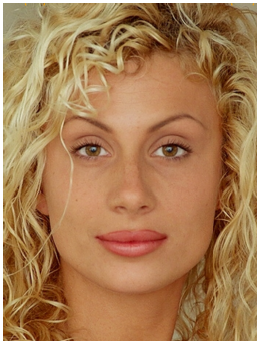
\includegraphics[scale=0.40]{Images/ea_data_visage_normal}}               
 \subfloat[Visage après traitement]{\label{fig:VisagesDataDef}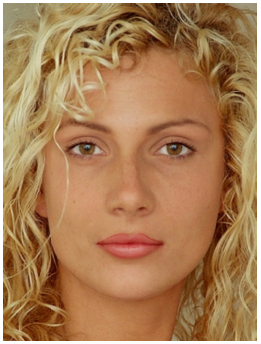
\includegraphics[scale=0.40]{Images/ea_data_visage_deforme}}
 \caption{Évolution d’un visage par déformation avec la méthode de Leyvand et al. \cite{Leyvand2008}}
 \label{fig:VisagesData}
\end{figure*}

Nous avons fait le choix de ne pas traiter la structure du visage d’une personne. L’image traitée doit au final être une version embellie de l’image originale. La contrainte éthique étant posée,  nous nous concentrerons sur l’amélioration de la peau du visage (en corrigeant les rides, acné \ldots) ainsi que le fond de l’image.
Le cadre des solutions étant défini, nous allons présenter dans la prochaine partie des propositions envisageables pour le projet.
\section{Nos propositions}
Dans cette section, nous allons présenter de manière succincte les deux solutions auxquelles nous avons pensé. A l’issue de cet exposé, un tableau récapitulatif comparera les propositions.
\subsection{Corriger les imperfections cutanées par le flou et une meilleure profondeur de champ}
\label{propun}
Nous avons dans un premier temps songé à nous intéresser au cas du fond. C’est un élément des photographies de portrait dont les méthodes des articles ne tirent pas profit. L’amélioration du fond sera conjuguée à celle du visage avec l’application d’un flou sur la peau à la manière de Lee et al. \cite{Lee}.
\paragraph{Objectifs}
L’objectif ici est d’améliorer simplement la photographie de portrait en mettant le sujet plus en valeur. Comme nous l’indiquons dans le résumé des méthodes à la fin du chapitre précédent, la technique de la profondeur de champ est assez peu utilisée alors qu’elle permet d’améliorer sensiblement la qualité de la photographie. Une fois le sujet mis en valeur, nous pourrions traiter la partie cutanée du visage afin de gommer la plupart des imperfections. Une photographie avec le visage embelli combiné avec un fond plus simple serait ainsi de meilleure facture.
\paragraph{Idées préliminaires}
Pour mettre en place cette solution, nous avons pensé à l'enchaînement suivant :
Nous pourrions émettre a priori des conditions préalables sur les photographies avant de les traiter. L’une d’elle est une photo avec peu de bruit. De plus l’image qui serait corrigée devra contenir un visage prépondérant, avec une orientation de face.
Le premier traitement à réaliser sur l’image serait la diminution du bruit si la condition n’a pas été respectée. Sa réduction peut passer par l’application d’un filtre passe-bas pour éliminer les pixels de couleurs aberrantes.
\paragraph{}
Dans le cas où tous les critères seraient conformes à ceux attendus, voici les étapes que nous suivrions pour cette solution:
\begin{enumerate}
\item Nous commencerions par rééquilibrer les couleurs en utilisant l’histogramme des couleurs et en réadaptant la balance des blancs.
\item La méthode de Lee  \cite{Lee} serait ensuite appliquée pour améliorer la peau du visage. Ce que l’on pourrait étendre concerne le fond. Il faut tout d’abord détacher le sujet (du buste aux cheveux) du fond, et appliquer sur ce premier un flou avec un certain coefficient, afin de le rendre plus indistinct et ainsi focaliser l’attention de l’observateur sur le visage.
\item Le sujet serait combiné avec l’image résultante précédente.
\end{enumerate}
\paragraph{}
En ce qui concerne les outils que nous pourrions utiliser pour réaliser ces étapes nous en avons relevés quelques-uns dans les articles. Pour détecter le visage, une méthode qui a été majoritairement utilisée est celle de Viola et Jones \cite{Viola2004}. Elle permet de détecter un visage dans une photo. Cette méthode est directement implémentée dans la bibliothèque de fonctions de Vision par Ordinateur OpenCV. Elle est aussi utilisée dans une boîte à outils de Matlab \copyright. Ensuite, dans cette zone un classifieur pourrait être utilisé pour identifier les pixels de peau.
Le lissage de la peau serait réalisé avec une combinaison des pixels de peau (enregistrés dans le masque) et une version floue de l’image. Une technique de flou connue est le flou gaussien par exemple.
Cette proposition étendant la méthode de Lee et al. \cite{Lee} s’intéresse donc au cas du fond et de la mise en valeur du sujet.
\subsection{Vers un embellissent optimal sans déformation du visage}
\label{propdeux}
Ce second point évoque un traitement plus poussé et performant des photographies.
\paragraph{Objectifs}
Dans cette approche, nous souhaiterions améliorer la qualité de la photographie au maximum de ce qu’il est possible de faire sans modifier la structure du visage.
\paragraph{Idées préliminaires}
Comme dans l’approche précédente, nous réaliserions des traitements sur le fond afin de le rendre plus beau puis nous appliquerions un flou afin d’en détacher le sujet. Une fois cela fait nous nous attaquerions au traitement du visage. Au niveau du traitement, nous commencerions par détecter les masque de pixels correspondant au visage, aux yeux, aux cheveux. Nous améliorerons le visage par le traitement des imperfections comme dans la méthode précédente puis nous embellirions l’éclat des dents et des cheveux.
Cette solution plus complexe à mettre en œuvre, pourrait produire des résultats intéressants à confronter avec les méthodes existantes.
\subsection{Conclusion et élection de la proposition suivie}
Nous avons dans le tableau ~\ref{tab:compprop} listé les avantages et inconvénients de nos propositions. De manière globale, la proposition ~\ref{propun} est plus réaliste en termes de temps de travail et d’utilisation d’outils existants. 

La proposition ~\ref{propdeux}, elle, dépend de nombreuses techniques de détection des défauts et de zones cibles, qui ne sont pas disponibles pour une grande partie. Combiner, trouver ou développer ces techniques serait un travail chronophage et requièrait une charge de travail bien supérieure. 
\paragraph*{}
C’est la raison pour laquelle, nous avons décidé de nous consacrer au développement de la première solution lors de la seconde phase de ce projet. Une fois ce choix réalisé, il nous reste à identifier plus précisément les techniques déjà implémentées
et à concevoir, plus formellement, la manière de mettre en œuvre cette solution.


\begin{table*}
\begin{center}
\begin{tabular}{|p{3cm}|p{4cm}|p{4cm}|p{4cm}|}
\hline
Proposition & Avantage & Inconvénient & Faisabilité \\ \hline
Corriger par flou et meilleure profondeur de champ & - Mise en valeur simple et efficace du sujet. Réalisable en utilisant OpenCV. Le traitement du fond n'a pas été traité dans l'existant. & - Il faut une technique pour séparer le sujet du fond & Faisable \\ \hline
Embellissent optimal sans déformation du visage & - Mise en valeur de la totalité du sujet. Cela représente la combinaison de la plupart des méthodes de l'existant (hormis celles qui changent la structure du visage). & - Nécessite beaucoup de détections et de corrections. Cette proposition sera donc beaucoup plus longue à exécuter. & Difficile \\ \hline
\end{tabular}
\end{center}
\caption{Tableau comparatif des propositions possibles}
\label{tab:compprop}
\end{table*}


\section{Correction par ajout de flou et augmentation de la profondeur de champ}
Nous avons choisi de nous intéresser à la première solution qui se concentre sur les imperfections du visage et au détachement du sujet de la photo par rapport au fond. Nonobstant, il reste quelques compléments bibliographiques à apporter avant d'aller plus loin. En effet, nous devons savoir comment la peau est sélectionnée actuellement, mais aussi savoir quelle piste nous devons explorer afin d'augmenter l'effet de défocalisation sur le fond. En plus de cela, il serait intéressant d'énoncer une manière d'évaluer les résultats obtenus.


\subsection{Détection des pixels de peau}
\paragraph*{}
Ce premier complément bibliographique s'axe sur la technique de classification des pixels de peau dans une image en couleur. Si dans le domaine RGB la classification est peu précise, d'autres domaines offrent plus de possibilité comme le YCrCb. Des chercheurs ont effectué des études sur les intervalles qui caractérisaient le mieux la couleur de la peau dans les différents canaux de l'YCrCb. Tout d'abord en 1999, Chai et Ngan \cite{Chai1999} ont déterminé que les intervalles suivants fonctionnaient bien: 

\begin{itemize}
\item 133 <= Cr <= 173;
\item 77 <= Cb <= 127.
\end{itemize}

\paragraph*{}
La composante Y n'était alors pas limitée, afin de ne pas mettre en jeu l'exposition dans les critères de sélection.
Puis en 2004, Kukharev et Nowosielski \cite{Kukharev2004} ont réajusté les intervalles de la sorte:

\begin{itemize}
\item 135 < Cr < 180;
\item 85 < Cb < 135;
\item Y > 80.
\end{itemize}

\paragraph*{}
Ces ajustements ont l'avantage de détecter plus correctement les pixels de peau puisque la composante correspondant à la luminance se voit bornée. L'ajout de seuils minimum et maximum permettent de ne pas être trop permissif lors de la sélection des pixels et d'éliminer quelques faux positifs mal éclairés. Par contre, les pixels de peau trop peu exposés ne sont plus considérés comme tels. La figure~\ref{fig:IntervalleMasquePeau1} compare les masques que l'on peut obtenir à partir d'un visage avec les deux intervalles proposés. On constate que le masque~\ref{fig:IntervalleMasquePeau1_Ancien} est plus pertinent que le masque~\ref{fig:IntervalleMasquePeau1_Nouveau} notamment en raison de la meilleure classification des cheveux par exemple.

\begin{figure*}[htp]
 \centering
 \subfloat[Visage Original]{\label{fig:IntervalleMasquePeau1_Original}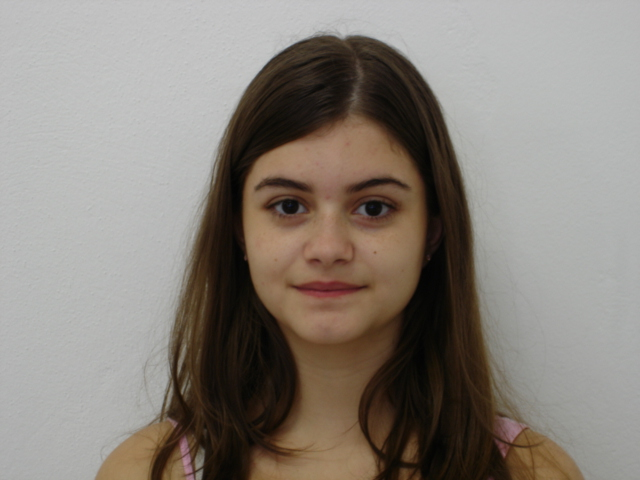
\includegraphics[scale=0.22]{Images/ea_peau_visage2_original}}               
 \subfloat[Masque de peau avec anciens intervalles \cite{Chai1999}]{\label{fig:IntervalleMasquePeau1_Ancien}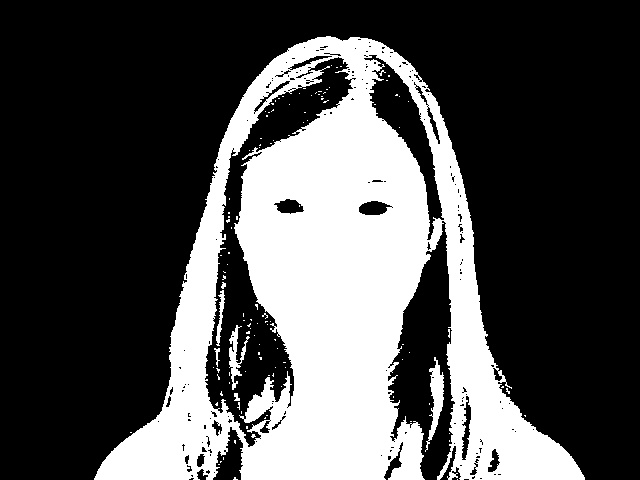
\includegraphics[scale=0.22]{Images/ea_peau_visage2_ancien_intervalle}}
 \subfloat[Masque de peau avec nouveaux intervalles \cite{Kukharev2004}]{\label{fig:IntervalleMasquePeau1_Nouveau}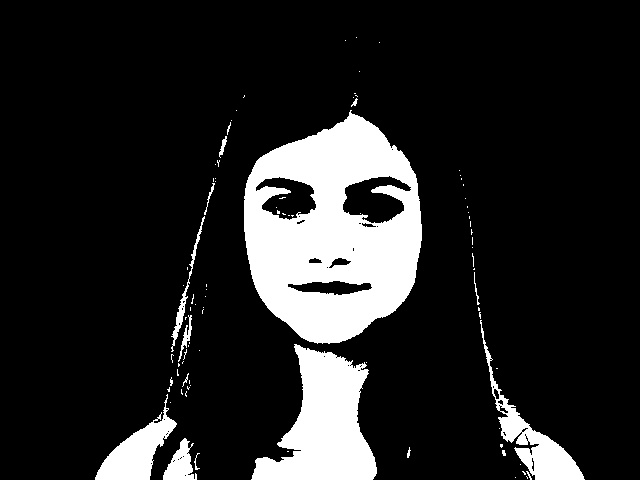
\includegraphics[scale=0.22]{Images/ea_peau_visage2_nouvel_intervalle}}
 \caption{Comparaison des masques de pixels de peau obtenus avec les deux intervalles pour un visage}
 \label{fig:IntervalleMasquePeau1}
\end{figure*}

\paragraph*{}
Nous avons choisi, à l'issue de ce point, d'utiliser la seconde version des intervalles en YCrCb pour la classification des pixels de peau.

\subsection{Augmentation de la profondeur de champ}
\paragraph*{}
La profondeur de champ est un critère qui, nous le rappelons, a été retenu pour qualifier les images de portrait. Ce critère est d'autant plus respecté quand le fond derrière le sujet est flou. Et nous avons opté pour la réalisation d'un traitement qui permettrait d'améliorer cet indice. Mais comment procéder  ?

\paragraph*{}
Premièrement, il faut tout d'abord segmenter l'image en entrée de la sorte: 
\begin{itemize}
\item pixels appartenant au fond;
\item pixels étant au premier plan.
\end{itemize} 

\paragraph*{}
Plusieurs méthodes existent pour différencier ces groupes de pixels. On peut utiliser pour segmenter une image plusieurs méthodes comme la segmentation basée sur la couleur, sur la construction de contours sur les objets les plus nets \dots. 
Après avoir expérimenté quelques unes de ces méthodes, nous n'avons pas obtenu de résultats concluants. Les zones étaient mal délimitées, et nous nous sommes rendus compte que certaines méthodes fonctionnent bien seulement si le fond est de type simple. Or, dans le cas d'images de portrait, le fond est potentiellement beaucoup plus complexe que de simples fonds uniformes.

\paragraph*{}
De ce constat, nous avons décidé de nous recentrer sur le traitement de Zhuo et Sim \cite{Zhuo2011} qui mesure la profondeur de champ. Pour estimer cet indice, leur méthode se base sur la construction d'une carte de profondeur. Étant donné que les codes Matlab\copyright qu'ils ont développés sont accessibles, nous avons décidé d'exploiter la carte de profondeur afin de segmenter l'image.

\paragraph*{}
Pour déterminer la profondeur moyenne à laquelle sont situés les pixels de la personne au premier plan, nous avons choisi d'exploiter la boite englobante du visage calculable à partir de la méthode de Viola et Jones. Il suffit alors de calculer la moyenne des valeurs des pixels de la carte de profondeur contenus dans la boite englobante. Cette partie est donc destinée à être implémentée sous Matlab\copyright.

\subsection{Correction du contraste et de la luminosité}

\subsection{Principe général de fonctionnement de la proposition}
\paragraph*{}
Maintenant que nous avons vu les différentes techniques utilisées dans la solution, intéressons-nous au traitement de manière globale.
\paragraph*{}
Le principe et la séquence d'application des traitements ont évolué depuis nos premières hypothèses dans le point~\ref{propun}. Si nous prenons en entrée une image et attendons en sortie une image corrigée automatiquement, les étapes pour y arriver ne sont plus dans le même ordre. Voici le nouveau principe:
\paragraph*{}
La première étape consiste à corriger les imperfections du visage.
Pour cela, il faut commencer par détecter le masque de peau du visage en nous basant sur la couleur caractéristique de la peau en YCrCb \cite{Kukharev2004}. 
Une fois celui ci en notre possession, nous le flouterons afin d'atténuer les traces de rides, cernes et autres imperfections cutanées. Ce flou est à appliquer en combinant la valeur originale des pixels de peau avec leur valeur floue moyennant l'usage d'un facteur d'opacité \cite{Lee}. Il existe plusieurs formes de flous qui peuvent être utilisés à cette fin comme le flou homogène, le flou gaussien, le flou médian ainsi que le flou bilatéral.
La grande difficulté de cette partie est ainsi de construire correctement le masque de peau. En effet, si ce dernier est trop large, nous prenons le risque de rendre flou des zones qui ne le devraient pas et de perdre du détail.
En sortie de cette première phase, nous obtenons, un visage lissé et paraissant plus jeune.
\paragraph*{}
Dans la seconde étape, nous nous attaquons à la défocalisation de l'image obtenue à la fin de l'étape précédente. Le but ici est de bien détacher le sujet du fond en renforçant l'effet de flou de ce dernier.
Nous utilisons une carte de profondeur \cite{Zhuo2011} pour déterminer à quelle distance se situe la composante principale de l'image (dans notre cas il s'agit du visage).
Ainsi, on ne conserve que la composante du premier plan dans sa version nette et on applique le noyau de flou sur le reste de l'image.
Le choix du noyau revêt une importance particulière car il ne faut pas qu'il soit trop fort pour rendre les objet indistinguables mais l'être assez pour permettre de réellement détacher la personne du reste de la photographie.
En sortie de cette étape, nous avons donc une image avec un sujet au visage lissé et bien séparé du fond de l'image.
\paragraph*{}
Dans la troisième et dernière étape, on corrige le contraste et la luminosité via la méthode expliquée dans le point précédent. 
Nous avons choisi d'intégrer cette étape à ce niveau de l'algorithme car il ne nous paraissait pas pertinent de réévaluer la couleur des pixels au départ pour ensuite les flouter.
Cette étape a pour but de corriger les erreurs d'exposition présentes de base sur la photographie comme notamment les cas des images sur ou sous-exposition. 

\subsection{Processus d'évaluation}



\paragraph*{}Cas des images à tester: 

Référence à la partie~\ref{part:PointEvaluation}.
La base FEI n'est pas adaptée pour des tests en dehors de la vérification du lissage de la peau.
Notre traitement est supposé améliorer des images de portrait avec des fonds plus complexes que les fonds uniformes de la base. La première raison à cela est que la base était destiné à un usage scientifique d'étude des visages. La seconde part simplement du principe que les utilisateurs préféreraient disposer d'une photo de profil qui fasse pas penser à une photo d'identité.

Donc nous avons recherché des images dans la base communautaire Flickr\copyright afin d'éprouver de manière plus efficace nos méthodes de différentiation du fond. La recherche que nous avons lancée contenait principalement le mot clé "selfie"\footnote{Selfie: désigne un autoportrait photographique} qui est un terme très en vogue actuellement.


\paragraph*{}
Méthode de test:
Quantitative pas possible

Qualitative : rapide sur les résultats obtenus avec trois critères : 
peau bien lissée
fond plus profond
contraste et luminosité plus adaptée





\section{Conclusion}









\chapter{Expérimentations et résultats}
\label{chap:Experimentations}


\section{Développements}

\begin{figure*}
\centering
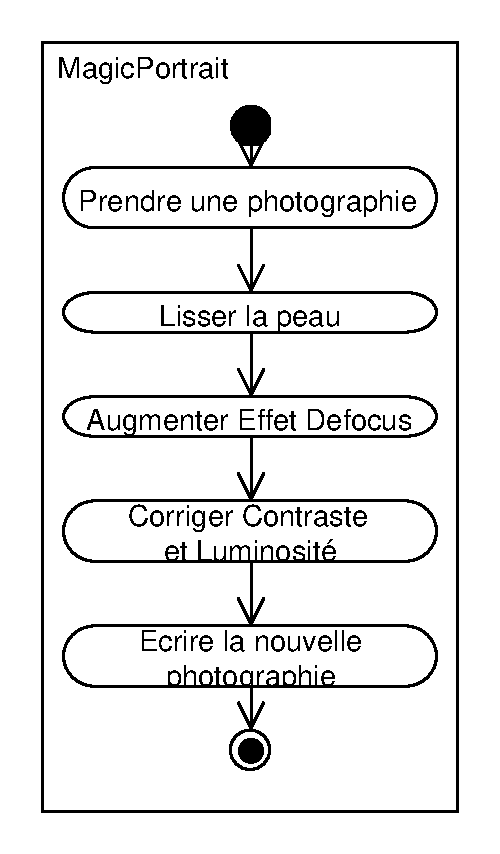
\includegraphics[scale=0.5]{Diagrammes/DiagrammeActivites_00_Global}
\caption{Diagramme d'Activités du fonctionnement global du projet}
\label{diag:diagramme00}
\end{figure*}

\subsection{Lissage de la peau}
\begin{figure*}
\centering
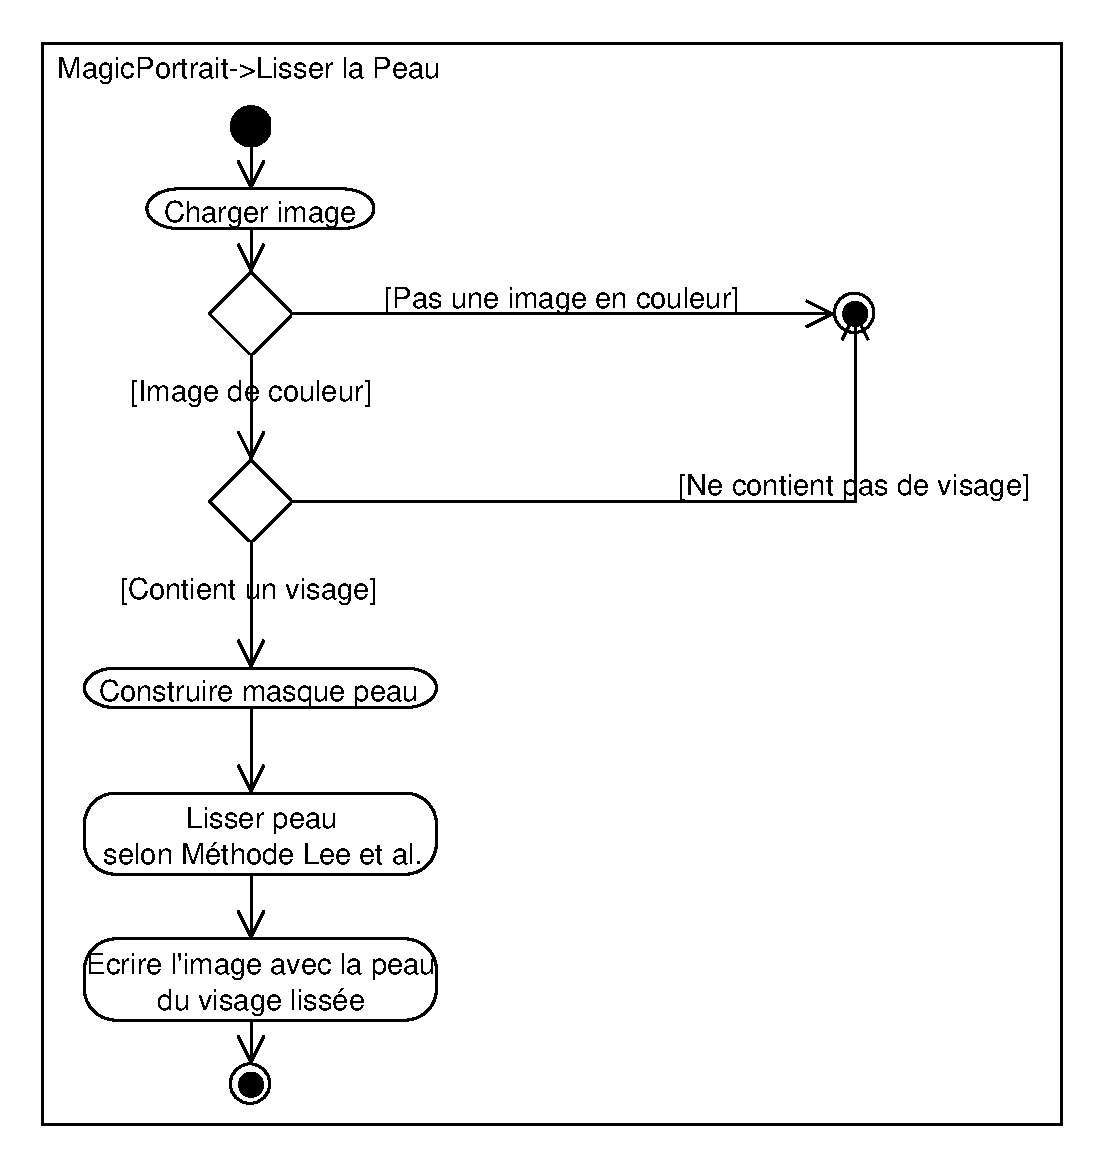
\includegraphics[scale=0.5]{Diagrammes/DiagrammeActivites_10_LissagePeau}
\caption{Diagramme d'Activités illustrant l'étape de lissage de la peau}
\label{diag:diagramme10}
\end{figure*}

\begin{figure*}
\centering
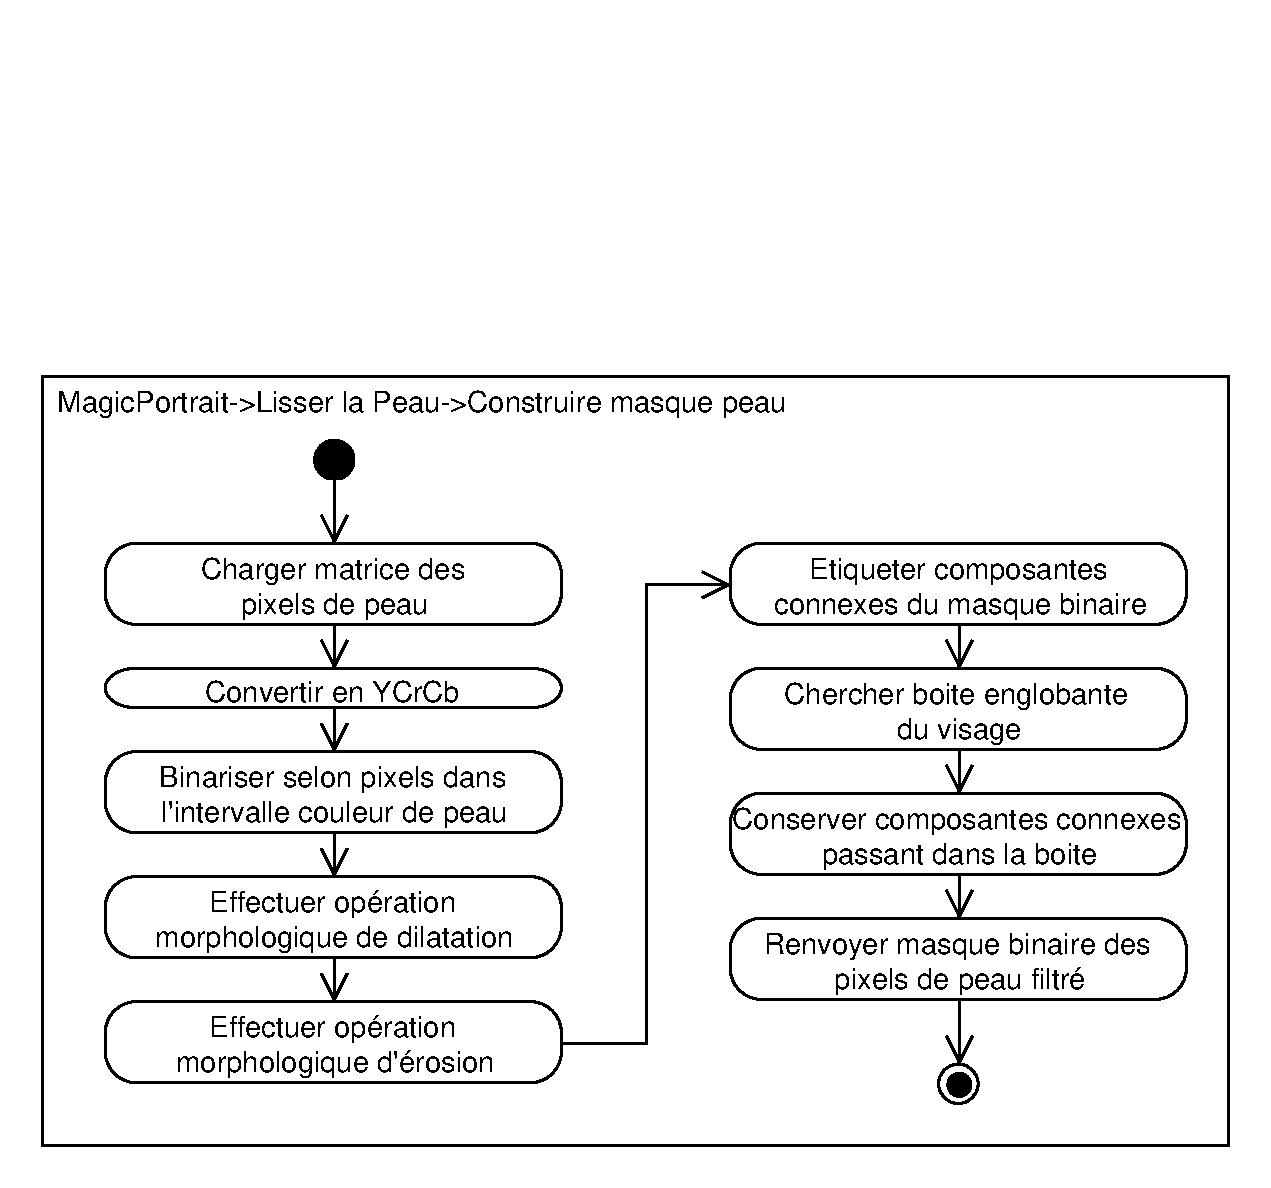
\includegraphics[scale=0.5]{Diagrammes/DiagrammeActivites_11_LissagePeau_Masque}
\caption{Diagramme d'Activités de la construction du masque des pixels de peau}
\label{diag:diagramme11}
\end{figure*}


\begin{figure*}[htp]
 \centering
 \subfloat[Masque Original]{\label{fig:MasquePeau01}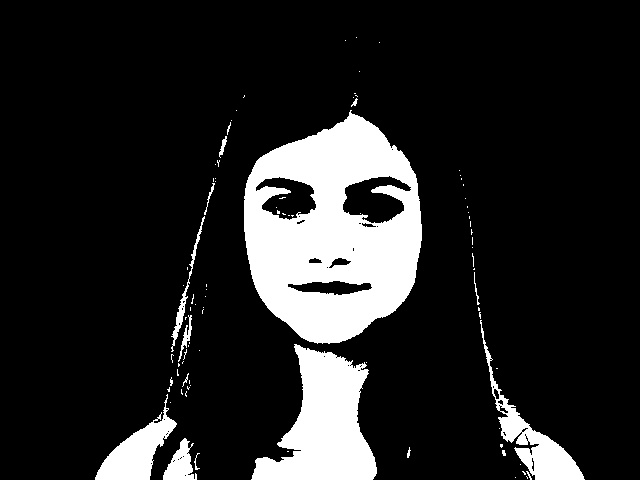
\includegraphics[scale=0.22]{Images/ea_masque_peau_01masque_simple}}               
 \subfloat[Après opérations morphologiques]{\label{fig:MasquePeau02}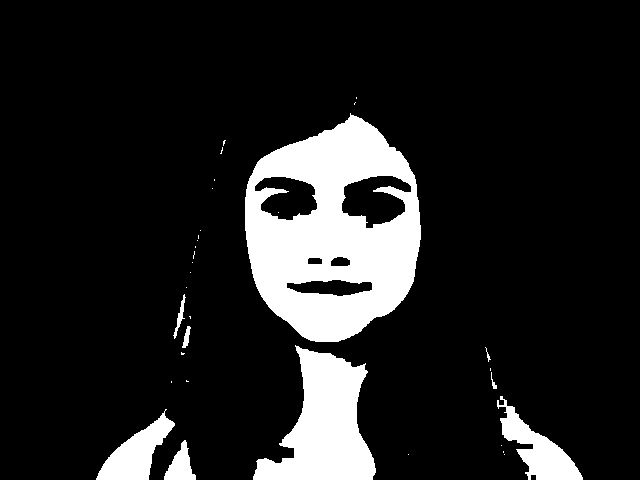
\includegraphics[scale=0.22]{Images/ea_masque_peau_02masque_operation_morpho}}
 \subfloat[Après filtrage sur composantes connexes]{\label{fig:MasquePeau03}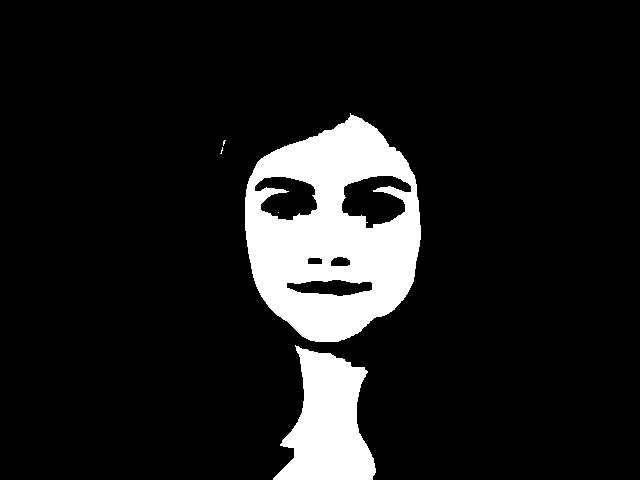
\includegraphics[scale=0.22]{Images/ea_masque_peau_03masque_propre}}
 \caption{Simplification d'un masque de pixels de peau}
 \label{fig:MasquePeau}
\end{figure*}





\subsection{Augmentation de la profondeur de champ}
\begin{figure*}
\centering
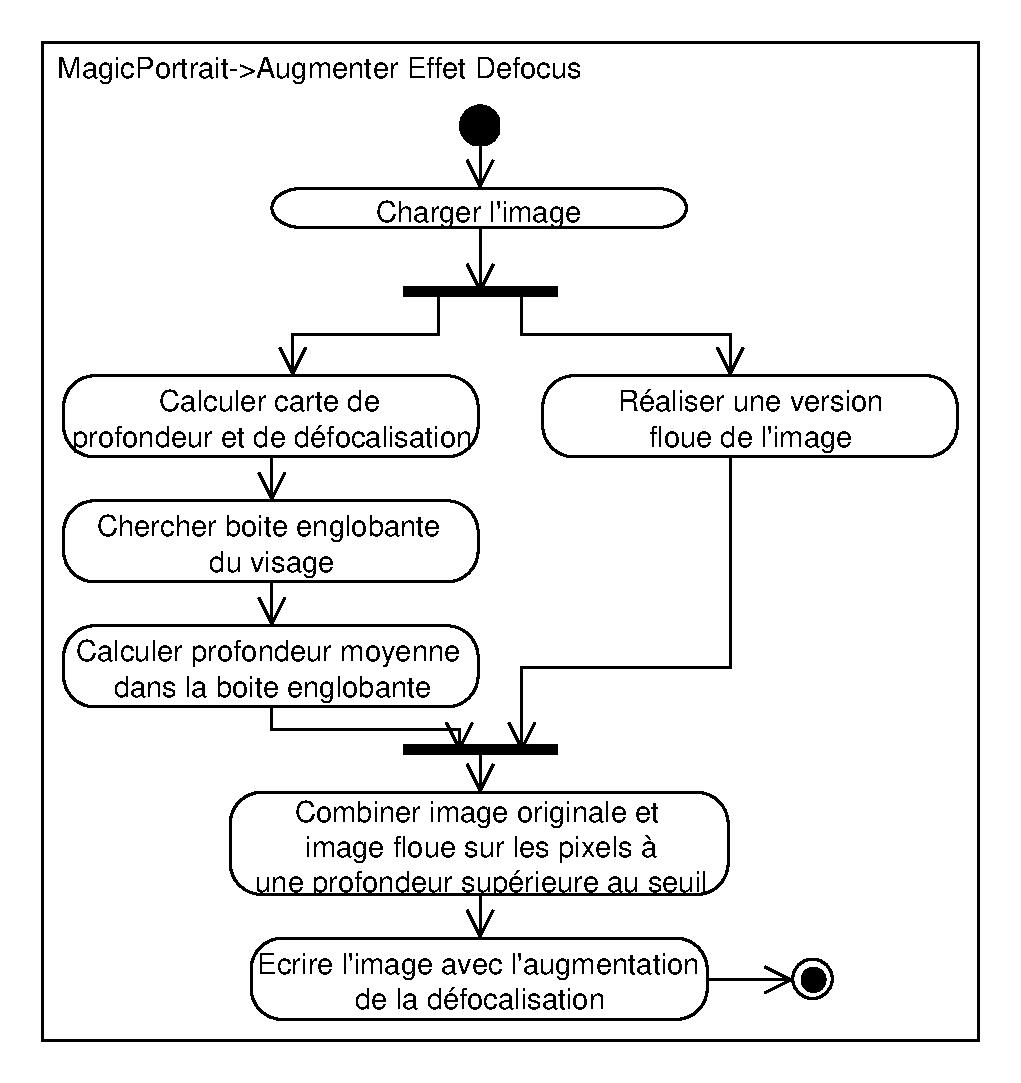
\includegraphics[scale=0.5]{Diagrammes/DiagrammeActivites_20_Profondeur}
\caption{Diagramme d'Activités illustrant le principe d'augmentation de l'effet de défocalisation}
\label{diag:diagramme20}
\end{figure*}

\subsection{Correction du contraste et de la luminosité}
\begin{figure*}
\centering
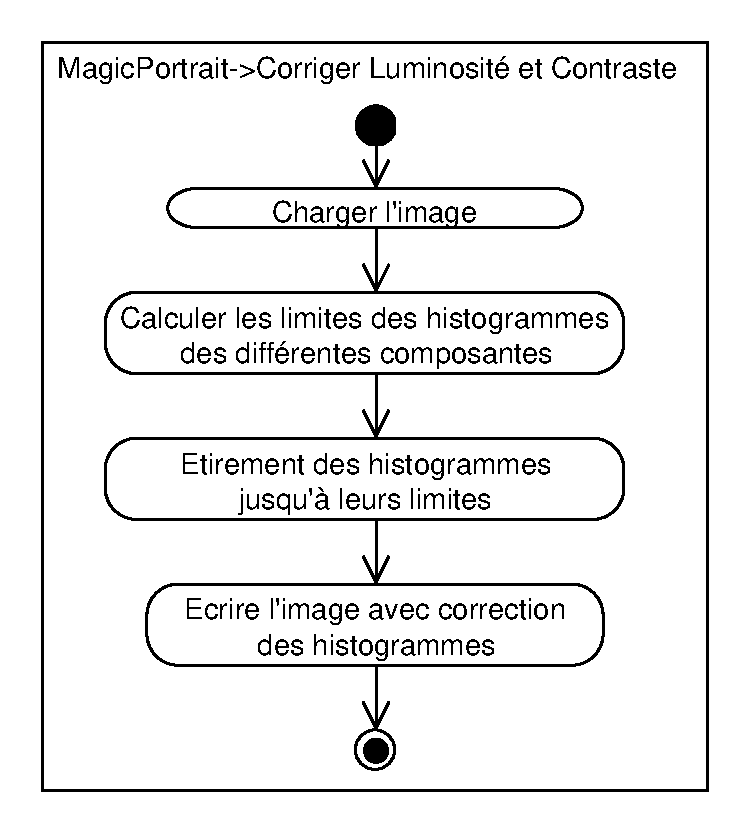
\includegraphics[scale=0.5]{Diagrammes/DiagrammeActivites_30_Contraste}
\caption{Diagramme d'Activités de la correction du contraste et de la luminosité}
\label{diag:diagramme30}
\end{figure*}

\section{Résultats}


\section{Interprétation et évaluation des résultats}

\section{Conclusion}





\chapter{Conclusion}
\label{chap:Conclusion}



\section{Résumé du travail effectué}

\section{Enseignements}

\section{Perspectives de recherche}










%---------------------------------------------------------------------------------------------------------
\bibliography{rapport}
\listoffigures{}
\listoftables{}
\appendix
\chapter{Fiches de lecture}
\label{ann:FichesLecture}
\section{\emph{An Algorithm For Automatic Skin Smoothing In Digital Portraits}}
L'article \cite{Lee} traite de l'amélioration de portraits numériques via un adoucissement de la peau.
\paragraph{Résumé}
Cet article s'inscrit dans le mouvement des techniques d'amélioration de portait numériques.
Plus particulièrement, il présente un algorithme réalisant une amélioration de la peau automatiquement.
Plusieurs étapes sont nécessaires pour réaliser ce traitement, à commencer par une phase de localisation du visage.
Tous les points d'intérêts sont tout d'abord enregistrés. Ensuite intervient une phase d'adoucissement de la peau.
Dans cette phase il faut créer un masque de pixels qui relèvent de la peau ou non.
Un GMM(Gaussian Mixture Model: Mélange de Modèles Gaussiens) est ensuite calculé sur chacun de ces masques.
Une fois cela effectué, intervient l'adoucissement à proprement parlé qui va lisser le visage sans affecter les détails du visage.
Les résultats de ce traitement sont revendiqués comme aussi réussis que ceux obtenus de manière manuelle avec des outils d'édition d'image.
\paragraph{Analyse}
Dans l'esprit des traitements manuels et semi-automatiques, cet algorithme automatique permet, en tout cas d'après les photos jointes à l'article, de constater un résultat similaire.
Les grandes étapes de l'algorithme sont communes à d'autres techniques d'imagerie, comme l'acquisition et le repérage des points d'intérêts.
Ce traitement du visage couvre une partie des améliorations possibles d'une photo de portrait.
\section{\emph{High Level Describable Attributes for Predicting Aesthetics and Interestingness}}
L'article \cite{Dhar}  présente une méthode de sélection automatique d'image parmi une grande collection afin d'en retirer les images qui seraient qualifiées de belles par un évaluateur humain.
\paragraph{Résumé}
Cet article nous présente trois grands groupes d'attributs utilisés par leur méthode pour rechercher d'aussi belles images qu'un humain.
Ces trois groupes d'attributs sont les attributs relevant de la composition (arrangements des objets et des couleurs), attributs liés au contenu (visages, type de scène), et les attributs correspondant à l'éclairage (naturel).
Une des expériences citées compare à partir d'une base d'apprentissage, les images retrouvées à partir des groupes d'attributs précédents avec les plus belles désignées par les humains. Les résultats sont décrits comme étant très proches d'un choix humain.
\paragraph{Analyse}
L'article démontre qu'un ordinateur entrainé à évaluer ces critères est capable de juger les photos de la même manière qu'un humain.
Il nous permet également d'en retirer des critères d'évaluation de plus ou moins haut niveau pour l'analyse de la beauté d'un portrait.
Nous avons pu voir que les attributs comme la règle des tiers, la profondeur du champ, couleurs complémentaires, présence de personnes ont un impact sur l'esthétique ressentie d'une photo.
\section{\emph{Data-driven enhancement of facial attractiveness}}
L'article Leyvand et al. \cite{Leyvand2008} traite de la problématique d'amélioration d'un portrait en utilisant la technique de déformation. Il traite également du problème du seuil de modification maximal au-delà duquel une photo n'est plus considérée comme fidèle à l'originale.
\paragraph{Résumé}
L'article présente les techniques utilisées pour réaliser une déformation du visage afin de le rendre  "plus beau" tout en restant fidèle à la photo originale. Pour cela, ils utilisent une base d'apprentissage évaluée par des utilisateurs.
L'algorithme va tout d'abord évaluer la beauté de l'image d'origine et retourner un vecteur avec la position des contours du visage. Avec ce vecteur, il va déterminer quelle image de la base est jugée plus belle et proche en termes de distance vectorielle. Il va alors retourner ce positionnement pour qu'on puisse modifier l'image d'origine en déformant l'image de manière à ce que le visage se retrouve à la position souhaitée.
\paragraph{Analyse}
Cet article peut être très utile car il traite d'une manière simple de l'amélioration de la beauté du portrait en repositionnant juste le visage. La problématique de modification et fidélité est aussi importante, car il nous faut savoir quand arrêter l'amélioration d'un portait.
\paragraph{Analyse}
Cet article peut être très utile car il traite d'une manière simple de l'amélioration de la beauté du portrait en repositionnant juste le visage. La problématique de modification et fidélité est aussi importante, car il nous faut savoir quand arrêter l'amélioration d'un portait.
\section{\emph{Method and system for enhancing portrait images that are processed in a batch mode}}
L'article \cite{Matraszek2004} nous présente un algorithme utilisé par un logiciel breveté afin d'améliorer localement un portrait.
\paragraph{Résumé}
\subparagraph{}
Cet article nous présente un algorithme qui va détecter les zones du visage et permettre à l'utilisateur de les modifier manuellement (choisir la “dose” de correction”). Ce logiciel est conçu pour être utilisé par un public non professionnel et est donc constitué de différentes jauges qui permettent d'augmenter ou de diminuer une valeur dans les zones ciblées. On dénombre quatre zones d'améliorations possibles : la peau, les yeux, les dents et la texture de la peau.
\subparagraph{}
En ce qui concerne l’essence de l’algorithme, le traitement est effectué en plusieurs étapes : détection du ou des visages présents dans l’image traitée, extraire les zones clés de chaque visage comme la peau, les yeux, le nez, la bouche, les sourcils, le cou, les cheveux. Les visages sont donc segmentés selon toutes ces caractéristiques analysées. A la suite de cela, pour chaque partie du visage a été développé un traitement correctif. Les paramètres de ces traitements sont déterminés automatiquement au moyen d’algorithme permettant d’obtenir le genre et l’âge du visage traité (au moyen d’une méthode utilisant une SVM).
Une amélioration des yeux citée pourrait être l’amélioration de la balance des blancs/ des couleurs de l’iris des yeux. Une présentation des principes des méthodes est réalisée dans la dernière partie de l’article.
\paragraph{Analyse}
Cet article nous permet de voir que des solutions payantes ont déjà été développées et nous donne une idée globale des améliorations réalisables. La solution proposée est donc un enchaînement d’améliorations donnant une image de meilleure qualité.
Cet article présente les calculs pour la plupart des techniques d’améliorations. On note cependant dans l'enchaînement, la présence d’un traitement de la texture de la peau qui altère la structure du visage. Si nous devions suivre le principe de la méthode présentée, nous ferions le choix de ne pas inclure ce dernier point.
\section{\emph{The Design of High-Level Features for Photo Quality Assessment}}
L'article \cite{Ke} nous présente un algorithme pour classifier une image. Cette méthode permet de déterminer informatiquement si une photo est de qualité professionnelle ou prise par un amateur.
\paragraph{Résumé}
Cet article présente les critères utilisés par les auteurs pour déterminer si une image semble réalisée par un professionnel ou non. Pour cela, ils utilisent des critères de haut niveau. Ces derniers sont basés sur l'observation des critères bas niveau généralement utilisés dans l'analyse d'image. Ils servent à corriger les problèmes observés lors de l'utilisation de ces critères bas niveau et apportent de nouvelles pistes de classification.
Tous ces critères haut niveau sont retirés uniquement à partir des caractéristiques de la photo et ne concernent pas les métadonnées de l'image.
Les critères retenus pour identifier une photo professionnelle sont :
\begin{itemize}
\item La simplicité, c'est à dire à quel point il est facile de détacher le sujet du fond. Plus c'est simple, plus la photo est de bonne qualité.
\item Le réalisme, c'est à dire à quel point la photo peut sembler atypique par rapport aux autres, la petite touche qui la rend différente.
\end{itemize}
C'est pour cela que dans l'algorithme les auteurs utilisent les caractéristiques suivantes qui référent directement aux critères listés plus haut :
\begin{itemize}
\item La distribution des bords. En analysant ce paramètres, on peut voir si le sujet se détache ou non du reste au niveau du centre de l'image. Cela permet d'analyse la simplicité.
\item Le nombre de nuances de couleurs dans l'image permet également de déterminer sa simplicité. Moins il y en a, plus la photo est professionnelle.
\item La distribution de couleurs. Plus il y en a, plus la photo est réaliste et à été prise avec soin.
\item Le niveau de flou, plus l'image est floue, moins bonne elle est.
\end{itemize}
En plus de ces critères haut niveau, ils vont également utiliser le contraste et l'éclairage.
\paragraph{Analyse}
Cet article nous sera utile pour la partie d'analyse de la qualité de l'image, notre but étant de permettre d'avoir un rendu "professionnel". Il nous permet de compléter les critères bas niveau que nous avions vus dans d'autres articles par des critères plus haut niveau. On y voit cependant la nécessité de conserver certains critères bas niveau qui sont essentiels à l'analyse de photo.
\section{\emph{Method of restoring closed eye portrait photo}}
L'article \cite{Li2011} présente une méthode qui permet de rectifier l'ouverture des yeux sur un portrait.
\paragraph{Résumé}
Lorsqu'on prend une photo, il arrive qu'on ait les yeux qui se ferment et de ce fait on a une drôle d'expression sur les photos. L'article présente une méthode afin de corriger ce problème en rectifiant l'ouverture des yeux.
Le principe est de détecter les yeux puis de voir s'ils sont ouverts ou fermés, de déterminer alors une zone de restauration si besoin et d'appliquer un des modèles prédéterminés pour leur rendre l'aspect ouvert.
L'article détaille l'algorithme utilisé pas à pas.
\paragraph{Analyse}
Ce genre de modification peut nous être utile pour notre projet car le cas d'yeux fermés ou partiellement fermés peut se présenter. Cela constitue donc une piste de réflexion intéressante (mais cela est peut-être trop ciblé sur le cas des yeux fermés, en effet, une photo que l'on ajoute pour son profil sur un réseau social est sujette à posséder des yeux ouverts).
\section{\emph{Studying Aesthetics in Photographic Images Using a Computational Approach}}
L'article \cite{Datta} traite de l'évaluation des critères esthétiques d'une photographie au moyen d'une approche informatique.
\paragraph{Résumé}
Les données sont issues d'un apprentissage statistique pour lisser les cas exceptionnels. Une base communautaire d'échange d'images est aussi utilisée. L'évaluation pourrait être biaisée par le fait que les personnes dont les notes sont prélevées sont majoritairement issues du monde de la photographie (amateurs et professionnels). L'article s'accorde sur le fait que les critères d'esthétiques pour un observateur humain relève du subjectif. Le but de l'article est de montrer qu'il y a des critères généraux qui ont un impact sur la "beauté" d'une photographie. La base de données d'images possède à l'origine deux points évalués, l'originalité et l'esthétique. Par soucis de corrélation de ces deux éléments, les auteurs ont choisi de ne traiter que le cas Esthétique.
Ensuite à partir de cette base, l'équipe a défini un classifieur qui distingue au niveau qualitatif les photos à partir de leurs critères bas et haut niveau (règle des tiers, saturation, exposition à la lumière et image colorée, taille et ratio, composition des couleurs des régions, ...)
La classification est effectuée avec un arbre de décision reprenant 15 parmi les 56 propriétés visuelles retenues par le laboratoire. Les résultats seraient en mesure de déterminer si une photographie serait jugée belle ou non par un humain.
\paragraph{Analyse}
Une nouvelle fois, cet article recoupe le sujet des critères jaugeant la beauté d'une photographie au sens général. Les traitements décrits dans l’article ont été réalisés avec Matlab\copyright.
\section{\emph{Automatic correction and enhancement of facial images}}
L'article \cite{Konoplev2012} propose un système de détection et de correction des défauts des visages contenus dans une photographie.
\paragraph{Résumé}
La technique prend en entrée une image et la change de référentiel couleur et passe de RGB vers le modèle de couleur CIELAB (désigné comme proposant des corrections douces et des couleurs plus naturelles). L'image passe ensuite dans un filtre lissant qui va réduire le bruit (sur l’ensemble de l’image). Les zones de peau sont à la suite reconnues et vont passer dans un nouveau filtre lissant pour les imperfections.
Le filtre utilise tout d'abord des paramètres spécifiques aux rides puis s'en suit un traitement similaire pour les rougeurs, boutons,.... Un histogramme des valeurs des couleurs caractérisant le visage est généré, il sert ensuite de base pour corriger la couleur des pixels des défauts (par la couleur la plus naturelle). Pour la distribution des couleurs caractérisant l'image, un modèle Gaussien est utilisé. L’image originale sert à l'image corrigée de base pour un autre ajustement (contraste, luminosité). L'image résultant repasse à la fin en RGB.
\paragraph{Analyse}
Ici, on peut noter l'intérêt de l'utilisation d'un autre espace de couleur, afin de ne pas être limité en RGB. Le traitement réalisé dans un espace de couleurs perceptuel permet d'obtenir des résultats plus naturels. La phase d'acquisition de la zone du visage et des zones à modifier est une nouvelle fois présente.
Le fait d’appliquer le filtre anti-bruit est un point que nous n’avons pas identifié dans toutes nos lectures et il serait utile de l’inclure (pour le cas de photographie dont la qualité ne serait pas optimale). D’autre part l’application du filtre lissant sur l’image intégralement pourrait altérer les détails.
\section{\emph{Natural Scenes Enhancement by Adaptive Color Correction}}
L'article \cite{Naccari} présente une méthode qui améliore le rendu des couleurs naturelles des portraits en utilisant un algorithme de correction des couleurs adaptatif.
\paragraph{Résumé}
Des études précédentes à cet article ont montré que ce qui importait dans une image en termes de couleur était les couleurs de la peau, du ciel et de la végétation. Ce sont ces points qui vont faire qu'un observateur va être plus attiré par une photo qu'une autre. Cet algorithme fonctionne en deux temps. La première partie de l'algorithme consiste à mettre un marqueur sur chaque pixel afin de déterminer à quelle catégorie précédemment citée il appartient. Pour cela, un algorithme de classification est utilisé. La seconde partie de l'algorithme va alors améliorer les couleurs s'il le juge nécessaire.
L'algorithme de classification a été entrainé par un jeu d'images préalablement labellisées et fait une décomposition dans l'espace HLS afin de séparer les pixels en différentes classes. Un filtre est ensuite appliqué au résultat pour corriger les pixels mal labellisés lors du passage.
La partie de correction de couleur fonctionne quant à elle, en réduisant la distance entre la couleur du pixel et la couleur de la classe cible à laquelle l'algorithme a déterminé qu'elle était rattachée.
\paragraph{Analyse}
Cet article peut nous aider en nous donnant des idées pour la classification des pixels du portrait.
On peut également y puiser des idées pour rendre la photo plus belle du point de vue de l'observateur sans rien modifier d'autre que les couleurs.
Cet algorithme a été testé sur différents types d'images dont des portraits et montre des résultats très satisfaisants, les observateurs préfèrent majoritairement les images améliorées par l'algorithme.
\section{\emph{Automatic Face and Skin Beautifiction using face detection}}
Un nouveau traitement automatique du visage et de la peau est présenté dans l’article \cite{Ciuc2010}.
\paragraph{Résumé}
La technique présente une amélioration de sous régions de l’image.  Elle repose sur une détection préalable de sous-régions du visage. Ensuite les zones choisies du visage sont améliorées au moyen d'un noyau lissant sur la luminance. L'image finale est une combinaison de certains pixels l'image originale avec ceux de la zone correspondante améliorée (pour un rendu plus naturel).
Ici le lissage sur la luminance dans les régions est soit la génération d’un flou, soit la réalisation d’une moyenne/approximation de la luminance, ou bien une combinaison des deux. De plus un filtre réduisant le bruit peut être appliqué sur une ou plusieurs régions selon le degré de dégradation.
L’espace de couleur utilisé lors des améliorations est l’YUV pour la séparation luminance/chrominance.
Au début dans la description des travaux traitant de sujets similaires, sont décrites comme peu performantes les méthodes de Kodak et P\& G utilisant des traitements globaux sur l'image (plutôt que sur des zones particulières comme le propose l’article).
\paragraph{Analyse}
La particularité de la technique ici est l’approche locale utilisée et non la globale que nous avons pu retrouver plusieurs fois. Les zones concernées (bouches et yeux principalement) peuvent subir plusieurs traitements pour supprimer les défauts de la prise de photo comme le bruit, les défauts intrinsèques du visage comme des yeux peu colorés ou des rides au niveau de la bouche.
Dans l’essentiel, les moyens utilisés sont l’application de flou et la modification de la luminance (techniques très souvent utilisées pour masquer les défauts et les estomper). L’article propose donc une alternative que l’on pourrait confronter aux autres dites globales.
\section{\emph{Machine à Vecteurs Supports Multi-Noyau pour la détection de points caractéristiques du visage}}
Nous avons lu cet article \cite{Rapp2012} par rapport à l’usage d’une autre technique d’apprentissage supervisé : les machines à vecteurs de support.
\paragraph{Résumé}
Ici l'essence de l'article parle de la détection de points caractéristiques du visage.
C’est un problème décrit comme étant non résolu pour le cas des visages variant beaucoup (manque de robustesse et de précision lorsque les expressions du visages changent ou lors de conditions de prise de photo mauvaises).
Il y a plusieurs catégories de méthodes de détection de points caractéristiques :
méthode d'alignement/détection conjointe/détection de points sans modèle global.
Le domaine d'application de la méthode est la détection des points caractéristiques sur des visages ayant des expressions différentes au moyen d’un SVM.
\paragraph{Analyse}
L’article présente une technique qui peut être utile pour les portraits avec des expressions qui varient selon les photos. D’après Wikipédia, les Machines à vecteurs de supports(SVM) sont un ensemble de techniques d'apprentissage supervisé (performance supérieure ou égale à celle des réseaux de neurones ou des modèles de mixture gaussienne).
\section{\emph{Segmentation des Traits du Visage, Analyse et Reconnaissance}}
Une partie de cet article\cite{Cognitives2006} traite de la détection des zones du visage comme le nez, la bouche. C'est la partie qui va nous intéresser.
\paragraph{Résumé}
\subparagraph{}
Pour détecter ces zones, les auteurs définissent des boites avec une taille prédéfinie. Il y a une boite pour l'intégralité du visage, une boite pour les yeux, une pour les sourcils. La taille de ces boites est calculée en faisant une moyenne sur un jeu d'apprentissage ou les zones en question ont été définies manuellement.
Pour déterminer les positions de ces boites sur le visage certains critères ont été posés en dur (yeux dans premier tiers du visage, œil gauche est dans la partie gauche, ...) et d'autres ont été calculées en faisant une moyenne sur le jeu d'apprentissage (distance entre les iris par exemple).
Une fois ces boites posées il ne reste plus qu'à détecter l'élément à l’intérieur.
L'article traite uniquement de la détection des yeux et des sourcils.
La thèse présente alors trois méthodes pour détecter ces éléments.
Tout d'abord la luminance/chrominance. Une étude révèle que les méthodes par apprentissage ne sont pas pertinentes pour obtenir une segmentation fine. On parle donc de reconnaissance des caractéristiques des portions de la photo. On utilise ainsi la luminance en supposant que les sourcils sont plus sombres que les pixels de peau environnants.
Une autre méthode consiste à définir que les yeux sont d'une autre couleur que la peau et si on trouve un bloc de couleur différente de la taille approximative des yeux alors on dit que c'est les yeux. On peut ensuite détecter le blanc de l'œil et les contours dans ce bloc.
\subparagraph{}
Une autre technique présentée est la détection de contours qui consiste à partir d'un pattern (motif) qui correspond à peu près à la forme des yeux et à le rendre modifiable pour qu'il détecte les formes. Cette méthode ne donne aucune garantie de réponse car l'évolution de la forme peut faire qu'au final on ne trouve rien, il n'y a pas de modèle d'évolution, c'est un processus indépendant.
Pour pallier à ce problème existe l'approche sous forme de Template déformable. Il s'agit du même principe mais cette fois les évolutions sont faites dans un sens respectant des caractéristiques observées de l'œil humain. La suite de la thèse présente une méthode qui fait un mix des trois approches et permet la détection d'expressions.
\paragraph{Analyse}
Le problème de la méthode de détection des sourcils (par différence de couleurs) c’est qu’elle repose sur la luminance de la photo et sous-entend bonne qualité dès départ.
Dans le cas de la recherche avec un motif déformable, une évolution forcée peut bloquer la détection des expressions faciales.
\section{\emph{Portrait beautification: A fast and robust approach}}
L'article \cite{Liu2007} présente un comparatif de méthodes pour pouvoir détecter un visage sur un portrait, séparer le visage de l'arrière-plan et enfin recoller le visage sur un autre arrière-plan. Il propose en parallèle un traitement à appliquer sur le visage afin de pouvoir rendre les couleurs de meilleure qualité si l'image n'est pas de bonne qualité à la base.
\paragraph{Résumé}
La première partie de l'article traite des trois techniques suivantes sur la segmentation de portraits (détecter la partie visage et la partie fond): Algorithmes génétiques, Algorithmes d'évolutions quantiques et pics d'histogramme. Chacun est présenté avec ses avantages et ses inconvénients.
Dans la seconde partie, on traite d'un algorithme pour la fusion d'image c'est à dire recoller la partie portrait sur un autre fond.
Dans la troisième partie, on traite d'un algorithme pour supprimer la déviation de couleur qu'aurais pu subir une image au moment de sa prise. La partie de détection du visage ne fait pas partie de cet algorithme et doit être réalisé avant de l'appliquer. L'algorithme en question fonctionne sur le principe de moyennes de pixels puis de comparaison à une table de valeur nommé "température de la couleur". Une fois qu'on a la tendance majoritaire de l'image, disons bleu par exemple, on calcule la déviation par rapport à la couleur normale et on corrige tous les pixels. Il s'agit d'un traitement global et non pas par régions.
\paragraph{Analyse}
Seul la première partie nous intéresse vraiment et elle n'offre pas de réponse claire à quel est le meilleur algorithme sur la segmentation, il est juste précisé que cela dépend des cas.
Dans la seconde partie la segmentation a été réalisée à l'aide d'un autre algorithme plus rapide mais qui perd en précision, le but étant d'illustrer uniquement la partie fusion. Cette partie ne nous apprend donc pas grand-chose.
La troisième partie en revanche illustre une technique pour pouvoir améliorer la couleur des portraits qui ont subis une déviation du à la mauvaise qualité de la prise de la photo.
Le fait qu'il n'y a pas de partie résultats statistiques ou de chiffres pour illustrer le taux de réussite de cet algorithme ne permet pas d'évaluer sa performance.
\section{\emph{Aesthetic Quality Assessment of Headshots}}
Cette proposition \cite{Males2013} est assez récente (septembre 2013) est traite de l’évaluation de la qualité esthétique d’une photographie de portrait.
\paragraph{Résumé}
Dans le domaine de la vision par ordinateur, les systèmes évaluant la qualité de photographie sont peu nombreux et pour ceux qui existent l’automatisme n’est pas une problématique systématique. La proposition présente une méthode automatique qui évalue cela au moyen de caractéristiques bas niveau ainsi que des critères haut niveau liés aux portraits. Ces différentes caractéristiques ou critères sont inspirés des règles suivies par le monde de la photographie professionnelle.
Un classifieur basé sur tous ces critères permet au final de distinguer les portraits attirants de ceux qui ne le sont pas. 10 critères ont été retenus car efficients :
\begin{itemize}
\item la netteté : basée sur deux facteurs (mesure spectrale sur l’ampleur de spectre local et une mesure spatiale sur la variation des maximums locaux)
\item la profondeur du champ : distance entre l’objet le plus proche et le plus éloigné dans la scène. Plus ce qui entoure le visage est flou plus le visage prend de l’importance (et le fond nous parait moins chargé). Ce critère est calculé en effectuant une distance entre la netteté de l’objet le plus proche avec celle qui est le plus éloigné.
\item la composition de la photo : la règle des tiers en fait partie. Cela permet d’avoir une image qui nous semble plus équilibrée
\item le contraste : c’est une différence de luminosité entre les parties les plus lumineuses de la photo avec les plus sombres. Le contraste gagne à être calculé dans l’espace HSV.
\item la clarté : dans le sens peu chargé. La clarté est calculée comme un pixel moyen à partir de l’espace de couleur HSL.
\item la coupure et la surexposition : la surexposition est calculé dans l’espace de gris de la photo. Elle est estimée comme le pourcentage de la zone du visage qui a ses pixels valués à la plus forte intensité (les plus clairs).
\item  le nombre de teintes : un trop grand nombre peut donner l’impression d’un portrait peu pensé et mal réalisé. Il faut un nombre de teintes raisonnables dans l’ensemble
\item la taille du visage : relatif à l’essence des photos de portrait. L’œil doit être attiré par le visage, il faut donc évaluer un ratio entre la zone du visage et la taille de l’image totale
\end{itemize}
L'expérimentation a été menée au moyen d’une séparation de la base de photos entre celles utilisées pour l’apprentissage (75\%) et celles utilisées pour les tests (25\%). Les visages ont été détectés au moyen de la méthode connue de Viola et Jones (dans la librairie OpenCV).
Les critères bas niveau sont calculés sur l’ensemble de l’image tels que le contraste et le nombre de teintes. Les critères haut niveau sont directement calculés dans la boite englobant le visage (détecté par la méthode de Viola et Jones). Une fois tous les critères calculés, ils sont normalisés et inclus dans un vecteur. Vecteurs qui vont alimenter le classifieur. Deux classifieurs ont été utilisés (pour faire une comparaison) il s’agit de SVM et d’AdaBoost. SVM a été en moyenne meilleur qu’AdaBoost.
Les avancées possibles pour cet article sont l’utilisation d’un meilleur outil de détection des visages ainsi qu’une méthode de détection des yeux.
\paragraph{Analyse}
Cet article apporte des précisions sur le cas particulier de la qualité des photographies de portrait où le visage est donc l’objet principal. Les 10 critères utilisés recoupent une grande partie des critères génériques applicables sur une photo classique. Le ratio sur la place qu’occupe le visage est par exemple la nouveauté de cet article.
Autre point intéressant il s’agit de la confrontation entre deux classifieurs par apprentissage supervisés que sont SVM et AdaBoost. L’un a l’air plus performant d’après les résultats de l’article. La bibliographie est aussi intéressante puisqu’elle cite des sources traitant l’évaluation de l’esthétique dans les portraits, les méthodes d’améliorations des portraits pour les photographes, les machines à vecteur de support ...


\chapter{Planification}
Cette partie est dédiée à la planification qui a été réalisée tout au long du projet.

\section{Phase I}
\subsection{Gantt Previsionnel}
Une fois le sujet affecté, nous avions fait une estimation des différentes phases que nous aurions à réaliser et du temps que chacune nous prendrait lors de la première phase. Tout est résumé dans la figure ~\ref{fig:PlanningPrevisionnel}.

\subsection{Gantt Effectif}
A l'issue de la première période nous avons conservé une vue du planning effectif. Le diagramme de Gantt effectif est représenté dans la figure ~\ref{fig:PlanningEffectif}. Dans le point suivant nous allons le comparer avec celui présenté précédemment et analyser la première phase.

\subsection{Comparaison des différences de planification de la première phase}
\paragraph*{}
Nous avions prévu les grandes phases suivantes : Choix du sujet, Acquisition du sujet, Étude bibliographique, Comparatifs sur l'état de l'art, Formulation propositions, Préparation soutenance, Soutenance Intermédiaire, Rédaction du Rapport

On peut voir que nous avons respecté ces différentes phases, il n’y a pas eu d’ajouts ou de suppressions à ce niveau-là. La seule différence se situe au niveau des dates où l’on constate un décalage d’environ une semaine. En effet, notre projet nécessitant une importante phase bibliographique, nous avons préféré y consacrer un peu plus de temps afin d’être sûr d’avoir fait le tour du sujet. Au final, nous arrivons quand même au même état final. Si on regarde la partie gestion des ressources, sur ces Gantts ne figurent pas les affectations des membres du binôme. Tout au long de la première phase, nous avons fait le choix de toujours travailler ensemble afin d’assurer que nous ayons la même base bibliographique pour pouvoir bien traiter la prochaine phase.

\paragraph*{}
La première phase nous a permis de dégager les conclusions suivantes en ce qui concerne la planification. Tout d’abord la gestion hebdomadaire des tâches est primordiale si nous voulons que chaque acteur du projet soit à jour. De plus, il ne faut pas prendre de retard sur les grandes étapes du projet, le cas échéant, il est plus difficile de gérer les imprévus qui pourraient survenir. 

\begin{figure*}
	\centering
		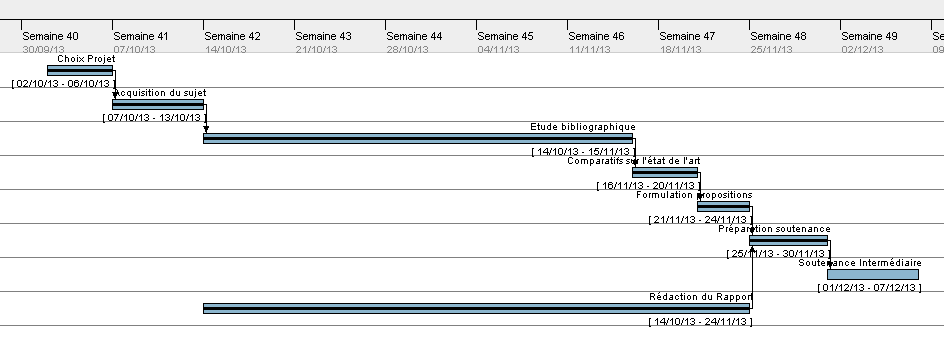
\includegraphics[width=1\textwidth]{Gantts/p1_previsionnel}
	\caption{Planification prévisionnelle Phase I}
	\label{fig:PlanningPrevisionnel}
\end{figure*}
\begin{figure*}
	\centering
		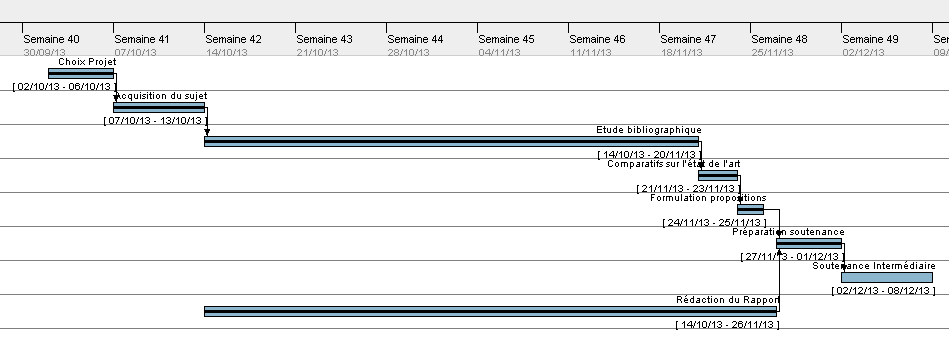
\includegraphics[width=1\textwidth]{Gantts/p1_effectif}
	\caption{Planning effectif Phase I}
	\label{fig:PlanningEffectif}
\end{figure*}



\section{Phase II}
\subsection{Gantt Previsionnel}
A l'issue de la première phase nous avons réalisé dans la figure~\ref{fig:PlanningPrevisionnel2} notre hypothèse de planification. Ce diagramme de Gantt, est centré sur le développement du projet.

\subsection{Gantt Effectif}
Maintenant que nous arrivons à la fin de la dernière phase, nous avons réalisé un nouveau diagramme de Gantt effectif ~\ref{fig:PlanningEffectif2}. Il illustre ce qui a été réalisé et nous pouvons constater des différences par rapport à ce qui était prévu.

\subsection{Comparaison des différences de planification de la seconde phase}

Comparaison des deux diagrammes. Comparaison des deux diagrammes. Comparaison des deux diagrammes. Comparaison des deux diagrammes. Comparaison des deux diagrammes  Comparaison des deux diagrammes. Comparaison des deux diagrammes. Comparaison des deux diagrammes. Comparaison des deux diagrammes. Comparaison des deux diagrammes. Comparaison des deux diagrammes. Comparaison des deux diagrammes. Comparaison des deux diagrammes. Comparaison des deux diagrammes. Comparaison des deux diagrammes. Comparaison des deux diagrammes.



\begin{figure*}
	\centering
		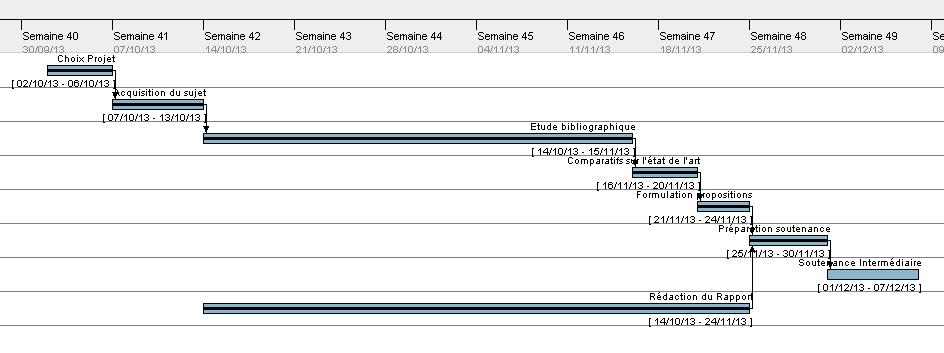
\includegraphics[width=1\textwidth]{Gantts/p2_previsionnel}
	\caption{Planification prévisionnelle Phase II}
	\label{fig:PlanningPrevisionnel2}
\end{figure*}
\begin{figure*}
	\centering
		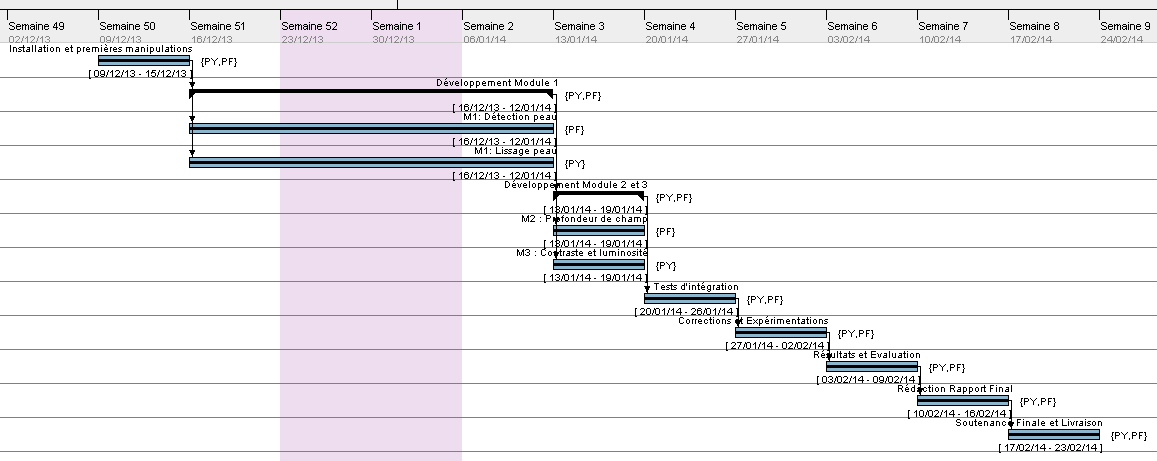
\includegraphics[width=1\textwidth]{Gantts/p2_effectif}
	\caption{Planning effectif Phase II}
	\label{fig:PlanningEffectif2}
\end{figure*}









\chapter{Fiches de suivi}
\label{ann:FichesSuivi}
\begin{fichesuivi}{30 septembre 2013}{6 octobre 2013}
	\tempstravailA{2}{30}
	\tempstravailB{2}{30}
\paragraph{}
	\begin{travaileffectue}
		\begin{itemize}
			\item Prise de contact avec plusieurs encadrants possibles : simple, réalisée à $100$ \% ;
			\item Etablissement de la liste des choix de sujets (24/23/48/44/22) : simple, réalisée à $100$ \% ;		
		\end{itemize}
	\end{travaileffectue}
	
\paragraph{}
	\begin{planification}
		\begin{itemize}
			\item Rencontrer le commanditaire pour lancer le projet à l'issu de l'affectation des projets
			\item Démarrer la partie bibliographique
		\end{itemize}
	\end{planification}
\end{fichesuivi}
\begin{fichesuivi}{07 octobre 2013}{13 octobre 2013}
	\tempstravailA{6}{00}
	\tempstravailB{6}{00}
\paragraph{}
	\begin{travaileffectue}
		\begin{itemize}
			\item Affectation au sujet 48 de PR\&D : simple, réalisée à $100$ \% ;
			\item Prise de contact avec l'encadrant du projet(Matthieu Perreira Da Silva) : simple, réalisée à $100$ \% ;
			\item Réunion de démarrage du projet avec Matthieu Perreira Da Silva : simple, réalisée à $100$ \% ;
			\item Préparation des outils de gestion de projet (mise en place d'un dépôt GitHub pour les rapports, et le code)  : simple, réalisée à $100$ \% ;
			\item Adoption de l'outil Mendeley pour la gestion des sources bibliographiques: simple, réalisée à $100$ \% ;
		\end{itemize}
	\end{travaileffectue}
\paragraph{}
	\begin{echange}
		\begin{itemize}
			\item Réception d'une liste d'articles à étudier de la part de Matthieu Perreira Da Silva mercredi ;
			\item Nous avons rencontré Matthieu Perreira Da Silva vendredi, pour en savoir davantage sur le déroulement du projet et ses attentes. L'objectif de la première phase qui est donc bibliographique est tout d'abord de déterminer ce qui est réalisé dans les différents domaines de l'amélioration d'image, de photo et de portrait. Pour cela il est possible que tous les articles ne soient pas des articles scientifiques, en ce qui concerne le domaine de la photographie. Par ailleurs, il nous faut très rapidement déterminer les limites de l'amélioration de photo de portrait étant donné qu'il faut savoir jusqu'à quelque point une photo peut être modifié pour rester fidèle.
			\item Matthieu Perreira Da Silva nous a aussi présenté différents outils pour la gestion de nos sources bibliographiques, ainsi que différents points d'accès aux articles scientifiques comme HAL, TEL, ACM, Springer,...
			\item Des rencontres régulières constitueront le point névralgique du suivi du projet, et une réunion devrait avoir lieu mardi 22 octobre. Avant cela la prochaine fiche devra être remise plus tôt.
		\end{itemize}
	\end{echange}	
	
\paragraph{}
	\begin{planification}
		\begin{itemize}
			\item Continuer la réalisation des fiches de lecture des premiers articles;
		\item Trouver de nouveaux articles à étudier;
			\item La prochaine fiche de suivi devra être rendu jeudi prochain;
		\end{itemize}
	\end{planification}
\end{fichesuivi}
\begin{fichesuivi}{14 octobre 2013}{20 octobre 2013}
	\tempstravailA{10}{00}
	\tempstravailB{10}{00}
\paragraph{}
	\begin{travaileffectue}
		\begin{itemize}
			\item Lecture des articles fournis par M Perreira Da Silva : simple, réalisée à $100$ \% ;
			\item Recherche de nos propres articles bibliographiques : simple, réalisée à $100$ \% ;
			\item Rédaction des parties introductives du rapport : simple, réalisée à $100$ \% ;
			\item Écriture des fiches de lecture correspondant aux articles : simple, réalisée à $100$ \% ;
		\end{itemize}
	\end{travaileffectue}
\paragraph{}
	\begin{echange}
		\begin{itemize}
			\item Prise de rendez-vous avec M Perreira Da Silva afin d'organiser une réunion d'avancement la semaine prochaine.
			\item Transmission des accès aux outils de gestion bibliographique mis en place.
		\end{itemize}
	\end{echange}	
	
\paragraph{}
	\begin{planification}
		\begin{itemize}
			\item Continuer à rechercher des articles bibliographiques.
			\item Continuer à remplir les fiches de lectures avec les nouveaux articles.
			\item Point d'avancement à réaliser.
		\end{itemize}
	\end{planification}
\end{fichesuivi}
\begin{fichesuivi}{21 octobre 2013}{27 octobre 2013}
	\tempstravailA{10}{00}
	\tempstravailB{10}{00}
\paragraph{}
	\begin{travaileffectue}
		\begin{itemize}
			\item Lecture de 4 nouveaux articles : simple, réalisée à $100$ \% ;
			\item Recherche de nouveaux articles : simple, réalisée à $100$ \% ;
			\item Réunion avec M. Perreira Da Silva jeudi  : simple, réalisée à $100$ \% ;
			\item Point de réflexion sur la future orientation du projet  : moyen, réalisée à $100$ \% ;
		\end{itemize}
	\end{travaileffectue}
\paragraph{}
	\begin{echange}
		\begin{itemize}
			\item Nous avons rencontré M. Perreira Da Silva jeudi après midi afin de faire un premier point sur la phase bibliographique. Lors de cette réunion nous avons revu les idées tirées des articles lus. Ce qu'il ressort de cette réunion est la nécessité de déterminer l'orientation du projet. En effet nous avons pour le moment des articles qui traitent d'amélioration de photographie, de visages dans des photos, de critères esthétiques... Or il nous faut choisir une cible de travail, et savoir ce sur quoi nous concentrerons la fin de la phase bibliographique. Le but du projet peut se différentier sur une amélioration de photo de portait sur un critère très précis (à pousser), un ensemble de critères, ou sur un aspect qui relève plus de l'évaluation.
			\item Il est clair que nous n'effectuerons pas d'opérations modifiant la photo originale telle que l'objet serait méconnaissable au retour. D'où l'importance de déterminer la limite de la manipulation de la photo en entrée.
			\item Le but à l'issue de la réunion est donc de déterminer vers quel type d'amélioration nous voulons aller pour pouvoir rechercher les outils, méthodes, techniques existantes afin de pouvoir les comparer et in fine émettre des propositions pertinentes.
		\end{itemize}
	\end{echange}	
	
\paragraph{}
	\begin{planification}
		\begin{itemize}
			\item Établir les fiches des derniers articles plus globaux ;
			\item Déterminer l'orientation du projet avant le début de la semaine de rentrée ;
			\item Étudier des articles en correspondance avec la nouvelle orientation ;
			\item Rechercher les outils traitant des problématiques relevées ;
			\item Contacter M. Perreira Da Silva pour lui faire part de notre choix ;
		\end{itemize}
	\end{planification}
\end{fichesuivi}
\begin{fichesuivi}{28 octobre 2013}{03 novembre 2013}
	\tempstravailA{1}{00}
	\tempstravailB{1}{00}
\paragraph{}
	\begin{travaileffectue}
		\begin{itemize}
			\item Nous avons discuté de la nouvelle orientation que souhaitions donner au projet de recherche. Nos premières lectures nous ont permis de cibler ce que nous voudrions traiter par la suite: moyenne, réalisée à $100$ \% ;
		\end{itemize}
	\end{travaileffectue}
\paragraph{}
	\begin{echange}
		\begin{itemize}
			\item Nous avons envoyé un mail à  M. Perreira Da Silva pour lui faire part de notre choix d'orientation. Les images en entrée seraient des “Photographies de type photo identité”
(avec prépondérance du visage). Les traitements qui nous intéressent
relèvent deux aspects:
- sur l’image de manière générale tels que liés à l’ Exposition,
Eclairage, Balance des blancs (traitements légers en vue de traitements
plus poussés sur le visage)
- sur le visage : comme la détection du visage, opérations de maquillage
pour masquer les signes tels que les rides, taches de rousseur, reflets,
acné. (Nous ne traiterons pas le cas des dents). Nous voulons aussi
étudier le cas du port d’objet type lunettes sur les traitements si cela a
déjà été réalisé.
Nous ne traiterons pas des opérations modifiant la structure du visage et
de la photographie	
		\end{itemize}
	\end{echange}	
	
\paragraph{}
	\begin{planification}
		\begin{itemize}
			\item La semaine de reprise nous allons centrer nos recherches sur les outils qui réalisent des améliorations automatique de photo de portrait  ;
		\end{itemize}
	\end{planification}
\end{fichesuivi}
\begin{fichesuivi}{04 novembre 2013}{10 novembre 2013}
	\tempstravailA{09}{45}
	\tempstravailB{09}{45}
\paragraph{}
	\begin{travaileffectue}
		\begin{itemize}
			\item Validation des fiches de lecture en attente : simple, réalisée à $100$ \% ;
			\item Lecture des derniers articles plus génériques de la première phase : simple, réalisée à $100$ \% ;
			\item Recherche et lecture d'articles, thèses traitant des améliorations locales du visage : moyenne, réalisée à $80$ \% ;
			\item Recherche d'outils réalisant des améliorations automatiques de portrait (dont la librairie OpenCV C++ pour la manipulation d'image, Makeup.Pho.to outil en ligne, PinkMirror outil en ligne mais avec sélection de zones manuelle, de nombreux outils proposaient simplement une amélioration basée sur une hausse de la luminosité de la photo pour gommer/masquer les défauts, ...) : moyenne, réalisée à $70$ \% ;
		\end{itemize}
	\end{travaileffectue}
\paragraph{}
	\begin{echange}
		\begin{itemize}
			\item M. Perreira Da Silva nous a envoyé un article auquel nous n'avions pas accès, à l'issue de notre mail de la semaine dernière.
		\end{itemize}
	\end{echange}	
	
\paragraph{}
	\begin{planification}
		\begin{itemize}
			\item Rattraper le temps manquant sur le projet (en raisons des jeux d'entreprise et du DS de Données Multimédia).
			\item Rédiger la partie bibliographique et mettre l'accent sur les techniques existantes permettant l'amélioration de photo de portrait (automatique).
			\item Comparer les différents outils
			\item Contacter M. Perreira Da Silva pour prendre un rendez-vous dans le courant de la semaine.
		\end{itemize}
	\end{planification}
\end{fichesuivi}
\begin{fichesuivi}{11 novembre 2013}{17 novembre 2013}
	\tempstravailA{15}{30}
	\tempstravailB{15}{30}
\paragraph{}
	\begin{travaileffectue}
		\begin{itemize}
			\item Recherche et lecture d'articles, thèses traitant des améliorations locales du visage : moyenne, réalisée à $100$ \% ;
			\item Mise à jour de quelques fiches de lecture (en ayant revu l’intérêt de certains articles qui seront utiles pour l’état de l’art): moyenne, réalisée à $100$ \% ;
			\item Passage en revu de tous les articles trouvés pour retirer les moins pertinents: longue, réalisée à $100$ \% ;
			\item Rédaction de la partie état de l’art : simple, réalisée à $20$ \% ;
\end{itemize}
	\end{travaileffectue}
\begin{travailnoneffectue}
		\begin{itemize}
			\item Pas d’avancé dans la recherche d'outils réalisant des améliorations automatiques de portrait : nous avons revu l’ensemble des documents stockés dans Mendeley et procédé à un tri de ces derniers;
		\end{itemize}
	\end{travailnoneffectue}
		
\paragraph{}
	\begin{planification}
		\begin{itemize}
			\item Continuer la rédaction de l’état de l’art et la terminer
			\item Comparer les différents outils, et les propositions effectuées dans l’état de l’art
			\item Rencontre M. Perreira Da Silva la semaine prochaine		
		\end{itemize}
	\end{planification}
\end{fichesuivi}
\begin{fichesuivi}{18 novembre 2013}{24 novembre 2013}
	\tempstravailA{12}{05}
	\tempstravailB{19}{30}
\paragraph{}
	\begin{travaileffectue}
		\begin{itemize}
			\item Rédaction de la partie résumé du rapport avec sa classification ACM : simple, réalisée à $100$ \% ;
			\item Mise à jour de la partie introductive du rapport : simple, réalisée à $100$%;
			\item Rédaction de la partie état de l’art : simple, réalisée à $70$ \% ;
			\item Rencontre avec M. Perreira Da Silva le mardi 19/11 : simple, réalisée à $100$ \% ;
		\end{itemize}
	\end{travaileffectue}
\begin{travailnoneffectue}
		\begin{itemize}
			\item Pas d’avancée notable dans la recherche d'outils implémentant des améliorations automatiques de portrait : toutes les méthodes que nous avons étudiées dans l’état de l’art n’ont pas fait l’objet d’implémentation		\end{itemize}
	\end{travailnoneffectue}
		
\paragraph{}
	\begin{echange}
		\begin{itemize}
			\item M. Perreira Da Silva nous a envoyé un nouvel article traitant de l'évaluation de la qualité esthétique des photos portraits. Cet article, qui est cette fois dédié à la photographie de portrait, apporte un complément sur ce que nous avions et permet d'affirmer certains critères qui sont apparus dans plusieurs articles.
			\item Nous avons eu une réunion mardi avec M. Perreira Da Silva. Lors de cette réunion, nous avons abordé plusieurs points.
			\item Nous hésitions sur la mise en forme de la partie sur les critères esthétiques dans l'état de l'art, et grâce à la discussion, nous les présenteront successivement et listeront les méthodes de calculs s'il y en a.
			\item Concernant la table listant les éléments bibliographiques, certaines entrées étaient peu complètes. Certaines entrées sous Mendeley n'avaient pas le bon type de document et certaines métadonnées étaient mal extraites.
			 \item Lors de la soutenance intermédiaire, le but est donc de présenter les critères d'évaluations esthétiques(et outils si possible) que nous avons identifiés. Une seconde partie sera dédiée aux propositions d'améliorations de photographie de portrait existantes. Chacun de ces points devra faire l'heure d'un comparatif avant de faire ressortir les avantages et limites de chaque approche.
			\item Toujours pour l'état de l'Art, il vaut mieux ne pas mettre de côté les traitements modifiant la structure des images afin de pouvoir mettre en avant les limites de ces solutions dans le comparatif et expliquer notre proposition.
			\item Au fil de nos lectures nous avons noté que pour la partie évaluation de la qualité des images, certains classifieurs fonctionnant au moyen d'un apprentissage supervisé, utilisaient des bases d'images pour l'entrainement et les tests. La question était de savoir si de telles bases étaient utilisées à Polytech. M. Perreira Da Silva nous a conseillé de nous pencher sur un rapport de projet de recherche de l'an dernier pour ce point. En effet le sujet traitant de la Beauté des Visages utilisait plusieurs bases de visages. Il s'agit des bases Karolinska et FEI. Une partie à ce sujet dans la partie évaluation de l'esthétique pourrait être utile, elle préciserait des méthodes d'évaluation globale et subjective(comme par exemple la possibilité de demander l'avis d'observateurs). Nous pourrions tout aussi bien effectuer des tests sur le trombinoscope de l'intranet.
			\item Nous nous sommes aussi intéressés aux outils pour manipuler les images et plus particulièrement permettant la détection de visages (en vue de pouvoir les améliorer). Nous avons lu que Matlab avait en 2012 mis à jour sa boite à outils pour la Vision par Ordinateur et que ses fonctions pouvaient être intéressantes. Il y a aussi la librairie OpenCV qui couplée au C++ peut donner de bons résultats. Nonobstant, M. Perreira n'est pas sûr que nous disposions de la toolbox Matlab. Après vérification, nous n'avons en effet pas cette toolbox disponible. Cette partie concernant les outils pour la manipulation peuvent apparaître dans la partie proposition mais ne devraient pas avoir une proportion très importante. En plus de cela, si nous le souhaitons plus tard, M. Perreira Da Silva peut nous envoyer du code Matlab pour estimer le flou d'une image.
			\item Dans la partie proposition, deux propositions pourraient être le bienvenu. En effet, nous pourrions présenter une approche que l'on pourrait de plus performante mais que nous ne pourrions mettre en place en raison de logiciels ou d'outils non disponibles, et une approche plus réaliste axée sur les manques d'une (ou d'une combinaison) des techniques existantes. 					
			\item Maintenant concernant le rapport, la rédaction se termine à la partie Propositions. Il ne faut pas oublier la partie auto-contrôle qui est à compléter.
		\end{itemize}
	\end{echange}		
		
\paragraph{}
	\begin{planification}
		\begin{itemize}
			\item Envoyer à M. Perreira Da Silva, au plus tard jeudi, une version bien avancée du rapport avant d'avoir un retour avant le rendu du dimanche 1er décembre.(état de l'art terminé, propositions formulées)
			\item Le diaporama sera aussi à réaliser afin de pouvoir compléter la fiche d'auto-contrôle
			\item Le Gantt effectif de la phase I est aussi à fournir
		\end{itemize}
	\end{planification}
\end{fichesuivi}
\begin{fichesuivi}{25 novembre 2013}{01 décembre 2013}
	\tempstravailA{26}{10}
	\tempstravailB{23}{20}
\paragraph{}
	\begin{travaileffectue}
		\begin{itemize}
			\item Fin de la rédaction de la partie état de l’art : simple, réalisée à $100$ \% ;
			\item Fin de la rédaction de la fiche d’auto-contrôle  : simple, réalisée à $100$ \% ;
			\item Rapport intermédiaire soumis à M. PERREIRA DA SILVA pour jeudi :  simple, réalisée à $100$ \% ;
			\item Modifications du  livrable intermédiaire suite aux commentaire de   M. PERREIRA DA SILVA : simple, réalisée à $100$ \% ;
			\item Rédaction du support de présentation pour la soutenance : simple, réalisée à $100$ \% ;
			\item Rendu du livrable intermédiaire  : simple, réalisée à $100$ \% ;
		\end{itemize}
	\end{travaileffectue}

\paragraph{}
	\begin{echange}
		\begin{itemize}
			\item Envoi du rapport intermédiaire à M. PERREIRA DA SILVA;
			\item Nous avons reçu les commentaires sur le rapport vendredi et avons modifié en conséquence ce que nous pouvions dans le temps restant;
		\end{itemize}
	\end{echange}
\paragraph*{}
	\begin{planification}
		\begin{itemize}
			\item La soutenance intermédiaire aura lieu le 4 décembre à 16h00;
			\item Pendant la semaine, l’objectif est de mieux se fixer les idées pour la méthode de sélection du fond d’une photographie avec un portrait.
		\end{itemize}
	\end{planification}
\end{fichesuivi}


\begin{fichesuivi}{2 décembre 2013}{8 décembre 2013}
	\tempstravailA{10}{10}
	\tempstravailB{10}{10}
\paragraph{}
	\begin{travaileffectue}
		\begin{itemize}
			\item Répétition pour la soutenance intermédiaire : simple, réalisée à $100$ \% ;
			\item Passage de la soutenance intermédiaire le 4 décembre : simple, réalisée à $100$ \% ;
			\item Correction du rapport à l'issue de la réception de sa version amendée par M. MARTINEZ (hors correction des champs manquants dans la bibliographie) :  simple, réalisée à $80$ \% ;
		\end{itemize}
	\end{travaileffectue}

\paragraph*{}
	\begin{planification}
		\begin{itemize}
			\item Etablir une planification plus précise de la phase de développement, en raison de la réduction du nombre de semaines restantes
			\item Installer OpenCV, Visual Studio pour de premières expérimentations et manipulations
		\end{itemize}
	\end{planification}
\end{fichesuivi}


\begin{fichesuivi}{9 décembre 2013}{15 décembre 2013}
	\tempstravailA{09}{45}
	\tempstravailB{09}{45}
\paragraph{}
	\begin{travaileffectue}
		\begin{itemize}
			\item Fin de la correction du rapport au niveau de la complétude des champs de la bibliographie:  simple, réalisée à $100$ \% ;
			\item Installation d’OpenCV et de Visual Studio: simple, réalisée à $100$ \% ;
			\item Premières expérimentations pour nous refamiliariser avec le C++ et utiliser OpenCV: simple, réalisée à $100$ \% ;
			\item Prise de rendez-vous avec Matthieu PERREIRA DA SILVA pour la semaine prochaine:  simple, réalisée à $100$ \% ;
		\end{itemize}
	\end{travaileffectue}

\paragraph*{}
	\begin{planification}
		\begin{itemize}
			\item Rencontrer M. PERREIRA DA SILVA pour faire le point post soutenance et expliquer ce que nous voulons mettre en place.;
			\item Commencer à implémenter, utiliser des briques existantes pour la détection de visages et de pîxels de peau;
		\end{itemize}
	\end{planification}
\end{fichesuivi}


\begin{fichesuivi}{16 décembre 2013}{22 décembre 2013}
	\tempstravailA{13}{00}
	\tempstravailB{13}{00}
\paragraph{}
	\begin{travaileffectue}
		\begin{itemize}
			\item Réunion d'avancement avec M. PERREIRA DA SILVA le 20 : simple, réalisée à $100$ \%;
			\item Premières expérimentations de détection de peau. La base d'images n'est pas adaptée pour les premières détections. La couleur du fond qui est uniforme, est trop proche de la couleur de la peau. Cela induit une mauvaise détection si on se base sur l'appartenance du pixel à un intervalle supposé englober un certain panel de couleurs de peau : simple, réalisée à $50$ \%;
			\item Premier essai de la méthode de Viola et Jones pour détecter la boite englobant le visage. La méthode fonctionne mais la boite est un peu trop petite pour contenir le visage intégralement : simple, réalisée à $70$ \%;
		\end{itemize}
	\end{travaileffectue}

\paragraph{}
	\begin{echange}
		\begin{itemize}
			\item Lors de la réunion avec M. PERREIRA DA SILVA, nous avons abordé tout d'abord la fin de la première phase. A l'issue de ce point, nous avons plus longuement discuté du déroulement de cette nouvelle phase. Actuellement les outils de développement sont en place (pour l'instant Visual Studio et OpenCV), et quelques expérimentations ont été effectuées. Cela a permis de détecter quelques pistes d'améliorations, notamment en ce qui concerne l'identification du masque de peau. Une piste d'amélioration pourrait être l'étude des densités de probabilités des pixels de peau contenus dans la boite englobant le visage. Un autre point à prendre en compte est la base d'images utilisée lors de la détection. En effet les images possèdent un fond trop proche de la couleur de la peau, ce qui induit une mauvaise détection. Une base d'images pour la détection de la peau plus adaptée doit être choisie;
			\item L'autre problématique de ce projet est l'amélioration de la profondeur de champ. Pour réaliser cela, nous devons tout d'abord segmenter l'image en termes de contenus au premier plan et de contenus à un plan plus éloigné. La segmentation couleur pourrait être utilisée pour identifier le sujet (cheveux+visage+buste,...), mais elle serait potentiellement plus aisée à mettre en place sous Matlab que sur OpenCV. De ce constat, le traitement final pourrait solliciter OpenCV et Matlab;
			\item De manière générale, ce projet sera divisé en deux temps. Nous devons en premier lieu, avec OpenCV, détecter et traiter les zones de peau. Puis dans un second temps, sous Matlab, il faudrait implémenter un module pour traiter le cas de la profondeur de champ;
			\item Une fois les congés terminés, un point sera à réaliser quant à l'avancement sur le premier module. 
		\end{itemize}
	\end{echange}

\paragraph*{}
	\begin{planification}
		\begin{itemize}
			\item Faire un retour à la rentrée sur l'avancement du projet à M. PERREIRA DA SILVA;
			\item Tout d'abord avancer au mieux possible le premier module d'amélioration de la peau;
		\end{itemize}
	\end{planification}
\end{fichesuivi}

\begin{fichesuivi}{6 janvier 2014}{12 janvier 2014}
	\tempstravailA{13}{00}
	\tempstravailB{13}{00}
\paragraph{}
	\begin{travaileffectue}
		\begin{itemize}
			\item Développement et intégration du premier module d’amélioration de la peau. A l’issue de quelques études pendant les congés, nous avons en conséquence cette semaine développé chacun de notre côté une partie dédiée à la détection de peau en se basant sur l’espace de couleurs YCrCb et une seconde partie dédiée au lissage de la peau à partir de la méthode de Lee et al. Ce module fonctionne tout d’abord par une détection des pixels relevant de la peau dans l’espace YCrCb, puis à partir de l’image sur laquelle on applique un filtre flou gaussien (de noyau plus ou moins grand) on combine la valeur des pixels de peau originale avec la valeur correspondant dans l’image modifiée. En respectant la méthode de Lee et al. ce seuil d’opacité est fixé à 50% afin que le lissage soit naturel  : moyen, réalisée à $100$ \%;
			\item Etude de fonction pour la segmentation couleur des images sous Matlab et OpenCV : simple, réalisée à $50$ \%;
			\item Etude d’un code d’estimation de la carte de Flou sous Matlab indiqué par M. Perreira Da Silva: simple, réalisé à $80$ \%;
		\end{itemize}
	\end{travaileffectue}

\paragraph*{}
	\begin{planification}
		\begin{itemize}
			\item La première partie d’amélioration de la peau étant terminé, nous nous concentrons à présent sur la seconde partie qui est la segmentation des éléments que l’on veut positionner au premier plan par rapport au fond sur lequel on appliquera un flou plus fort.		
\end{itemize}
	\end{planification}
\end{fichesuivi}

\begin{fichesuivi}{13 janvier 2014}{19 janvier 2014}
	\tempstravailA{12}{00}
	\tempstravailB{12}{00}
\paragraph{}
	\begin{travaileffectue}
		\begin{itemize}
			\item Nous avons continué cette semaine à traiter les phases d'amélioration de la profondeur de champ et de correction du contraste et de la luminosité. Nous avons étudié ces deux points sous Matlab cette fois-ci pour des raisons plus pratiques. Pour réaliser notre première version du traitement d'amélioration de la profondeur de champ, nous avons utilisé des codes Matlab développés pour dresser une carte de profondeur (Defocus Estimation).On calcule une image floue (de type disque pour le différencier du flou gaussien de la peau), puis à partir de la carte obtenue, on peut conserver la version floue d'un pixel si sa profondeur est supérieur à celle que l'on observe en moyenne dans la zone dessinée par la boite englobant le visage par Viola et Jones. Les premiers résultats sont mitigés car selon les images, une partie du visage est estimée dans un plan de profondeur similaire au fond rendant la séparation difficile :moyenne, réalisée à $60$ \%;
			\item Nous avons aussi voulu étudier la segmentation d'une image en termes de couleurs et de parties connexes pour pouvoir "floutter" tout ce qui est hors du visage+corps+cheveux mais nos études ne sont encore pas assez poussées: moyenne, réalisée à $40$ \%;
			\item A l'issue de nos recherches pour l'amélioration du contraste et de la luminosité, nous avons lu un article proposant d'améliorer les composantes de l'image dans l'espace HSV. Des algorithmes Matlab que nous avons adaptés, produisent des résultats qui nous semblent corrects, cependant le temps de calcul est assez important(25 secondes de traitement pour une image de 500x700 pixels) : moyenne, réalisée à $70$ \%;
		\end{itemize}
	\end{travaileffectue}

\paragraph{}
	\begin{echange}
		\begin{itemize}
			\item Nous avons rencontré M. Perreira Da Silva lundi après-midi et lui avons montré nos travaux de lissage de peau. Les points à améliorer sont la taille du noyau utilisé pour le flou, ainsi que la classification des pixels de peau. Cette classification peut sélectionner des pixels assez éloignés du visage et cela induit des zones qui ne devraient pas être lissées . Pour corriger cela, il faudrait s'intéresser aux composantes connexes et profiter de la boite de Viola et Jones.
		\end{itemize}
	\end{echange}


\paragraph*{}
	\begin{planification}
		\begin{itemize}
			\item Améliorer la construction du masque des pixels de peau afin de ne conserver de manière générale que la composante connexe que l'on retrouve dans la boite de Viola et Jones. Cela permettrait d'éliminer certaines erreurs de classification.
			\item Continuer nos travaux sur l'amélioration du fond car les résultats ne correspondent pas encore à nos attentes. De plus les temps de calculs sont particulièrement longs (et une personne lambda possède des images qui peuvent potentiellement être au minimum quatre fois plus grandes).	
\end{itemize}
	\end{planification}
\end{fichesuivi}

\begin{fichesuivi}{20 janvier 2014}{26 janvier 2014}
	\tempstravailA{07}{00}
	\tempstravailB{11}{00}
\paragraph{}
	\begin{travaileffectue}
		\begin{itemize}
			\item Nous avons réalisé des scripts batch afin d'automatiser l'exécution de la chaîne de  traitements de nos différents codes C++ et Matlab. Cela permettra de lancer sur un lot d'images le traitement de manière plus automatique, moyenne, $100$\%;
			\item Nous avons modifié l'architecture de nos codes C++ et Matlab afin de les rendre plus clair et de documenter en vue du dépôt final: moyenne, réalisée à $100$ \%;
			\item Nous avons continué à modifier les scripts Matlab pour la défocalisation du fond et le code C++ pour le lissage de la peau mais les résultats ne sont pas encore satisfaisant, moyenne, $20$ \%;
		\end{itemize}
	\end{travaileffectue}


\paragraph*{}
	\begin{planification}
		\begin{itemize}
			\item Terminer la correction du lissage du visage et éliminer les erreurs de flou du fond qui altèrent la couleur.
			\item Nous souhaitons achever la partie développement du projet la semaine prochaine afin d'avoir une semaine de bilan, de documentation et de finalisation du rapport.
\end{itemize}
	\end{planification}
\end{fichesuivi}

\begin{fichesuivi}{27 janvier 2014}{02 février 2014}
	\tempstravailA{25}{30}
	\tempstravailB{24}{30}
\paragraph{}
	\begin{travaileffectue}
		\begin{itemize}
			\item Nous avons amélioré la construction du masque de peau pour le lissage. Nous avons étiqueté les composantes connexes du masque initial, puis nous avons conservé toutes les composantes connexes qui passaient au moins dans la boite englobant le visage afin d'éliminer une partie des faux positifs: difficile, $100$ \%;
			\item En ce qui concerne l'amélioration du contraste et de la luminosité, nous avons changé de méthode. Auparavant, le travail était réalisé dans l'espace HSV et le temps de calcul était trop long. Nous avons donc pensé à une autre technique reprenant la méthode de "stretching" d'histogramme. Cette technique va rééquilibrer les histogrammes des composantes de l'image afin qu'ils occupent toute la plage de valeurs disponibles. Le résultat est obtenu de manière bien plus rapide et nous semble meilleur : moyenne, $100$ \%;
			\item La dernière modification est celle de la séparation du fond et de la personne au premier plan. Nous avons revu certains paramètres de notre traitement afin d'obtenir un seuil de profondeur plus judicieux, de plus, nous avons intégré un peu d'opacité avec le flou que nous rajoutons sur le fond afin d'avoir un résultat plus naturel. Les résultats semblent indiquer que les images ont le fond qui se détache plus facilement si dès le départ il y a un peu de flou. En effet nous utilisons la carte de profondeur de l'image et si cette dernière n'a pas de fond un peu flou, il est compliqué d'augmenter l'effet de défocus. Il s'agit d'une des limites de l'approche mise en place. Une autre critique est le temps de traitement qui est assez long pour les images ayant une dimension supérieure à 500 pixels. Au delà, le temps peut être compté en vingtaine de minutes (et plus encore selon la taille de l'image).
L'utilisation de Matlab s'avère être assez coûteuse et l'implémentation gagnerait à être migrée en C++ pour le gain de vitesse.Nous n'avons plus le problème de couleurs qui déteignent et le flou est renforcé : difficile, $100$ \%;
		\end{itemize}
	\end{travaileffectue}


\paragraph*{}
	\begin{planification}
		\begin{itemize}
			\item Faire un point avec M. Perreira Da Silva sur la fin du développement
			\item Prendre des images supplémentaires avec un fond plus complexe et éprouver notre traitement.
			\item Terminer la documentation des codes, et avancer le rapport final.
\end{itemize}
	\end{planification}
\end{fichesuivi}

\begin{fichesuivi}{03 février 2014}{09 février 2014}
	\tempstravailA{11}{00}
	\tempstravailB{11}{20}
\paragraph{}
	\begin{travaileffectue}
		\begin{itemize}
			\item Dernières corrections des codes C++ et Matlab  : moyenne, $100$ \%;
			\item Réalisation des diagrammes d’activités principaux illustrant l’enchaînement des différents codes développés : simple, $100$ \%;
			\item Lancement de nos codes d’améliorations sur 22 images différentes afin d’étudier les résultats du traitement  : simple, $100$ \%;
			\item Rencontre avec M. Perreira Da Silva pour faire un point de fin de développement et sur les résultats  : simple, $100$ \%;
		\end{itemize}
	\end{travaileffectue}


\paragraph{}
	\begin{echange}
		\begin{itemize}
			\item Au cours de notre rencontre avec M. Perreira Da Silva cette semaine, nous avons abordé les résultats et discuté des images pour lesquelles le traitement fonctionne bien et celles pour lesquelles on constate quelques limites.
			\item Tout d’abord la première limite est la constitution du masque des pixels de peau qui aurait gagné à être personnalisé et construit sur la base de chaque image. Cela aurait pu se faire en calculant la couleur moyenne des pixels de peau dans la boite englobante du visage. Or, notre méthode utilise des bornes assez “génériques” qui peuvent se révéler insuffisantes comme nous avons pu le constater sur certaines images.
			\item Ensuite vient l’augmentation de la profondeur de champ. Notre méthode s’appuie sur la détection de la profondeur des pixels dans l’image et le renforcement de cet effet. Incidemment, s’il y a peu de profondeur dans l’image, le traitement sera peu efficace et visible..
	\item Pour ce qui est de la dernière étape, la correction du contraste et de la luminosité, les résultats sont très corrects à l’exception d’un changement de couleur que nous avons remarqué et d’une correction rendant l’image moins “belle” qu’auparavant. Mais dans l’ensemble, c’est une partie du traitement qui fonctionne bien.
	\item En dehors de ce point sur les résultats, nous avons aussi parlé du rapport final et du point sur l’évaluation des résultats. Si une évaluation quantitative n’est pas possible dans le temps imparti, nous évaluerons de manière qualitatif les images que nous avons corrigées et identifierons les limites du traitement.
		\end{itemize}
	\end{echange}

\paragraph*{}
	\begin{planification}
		\begin{itemize}
			\item Terminer le rapport du projet pour la partie 
			\item Préparer la procédure de recette en prévision de la dernière semaine
\end{itemize}
	\end{planification}
\end{fichesuivi}




\newpage
\printweeksummary
\chapter{Auto-contrôle et auto-évaluation}
La figure~\ref{fig:AutoEvaluationTravailIntermediaire} présente l'auto-évaluation que nous avons réalisée pour la première partie du projet de recherche. La figure ~\ref{fig:AutoEvaluationTravailFinal} concerne la seconde partie du projet.
\begin{figure*}
	\centering
     \ifscreen % macro TeX (issue de la classe report-rd-info.cls) permettant d'ajuster le contenu en fonction du l'orientation du document (<< screen >> ou pas)
        \rotatebox{90}{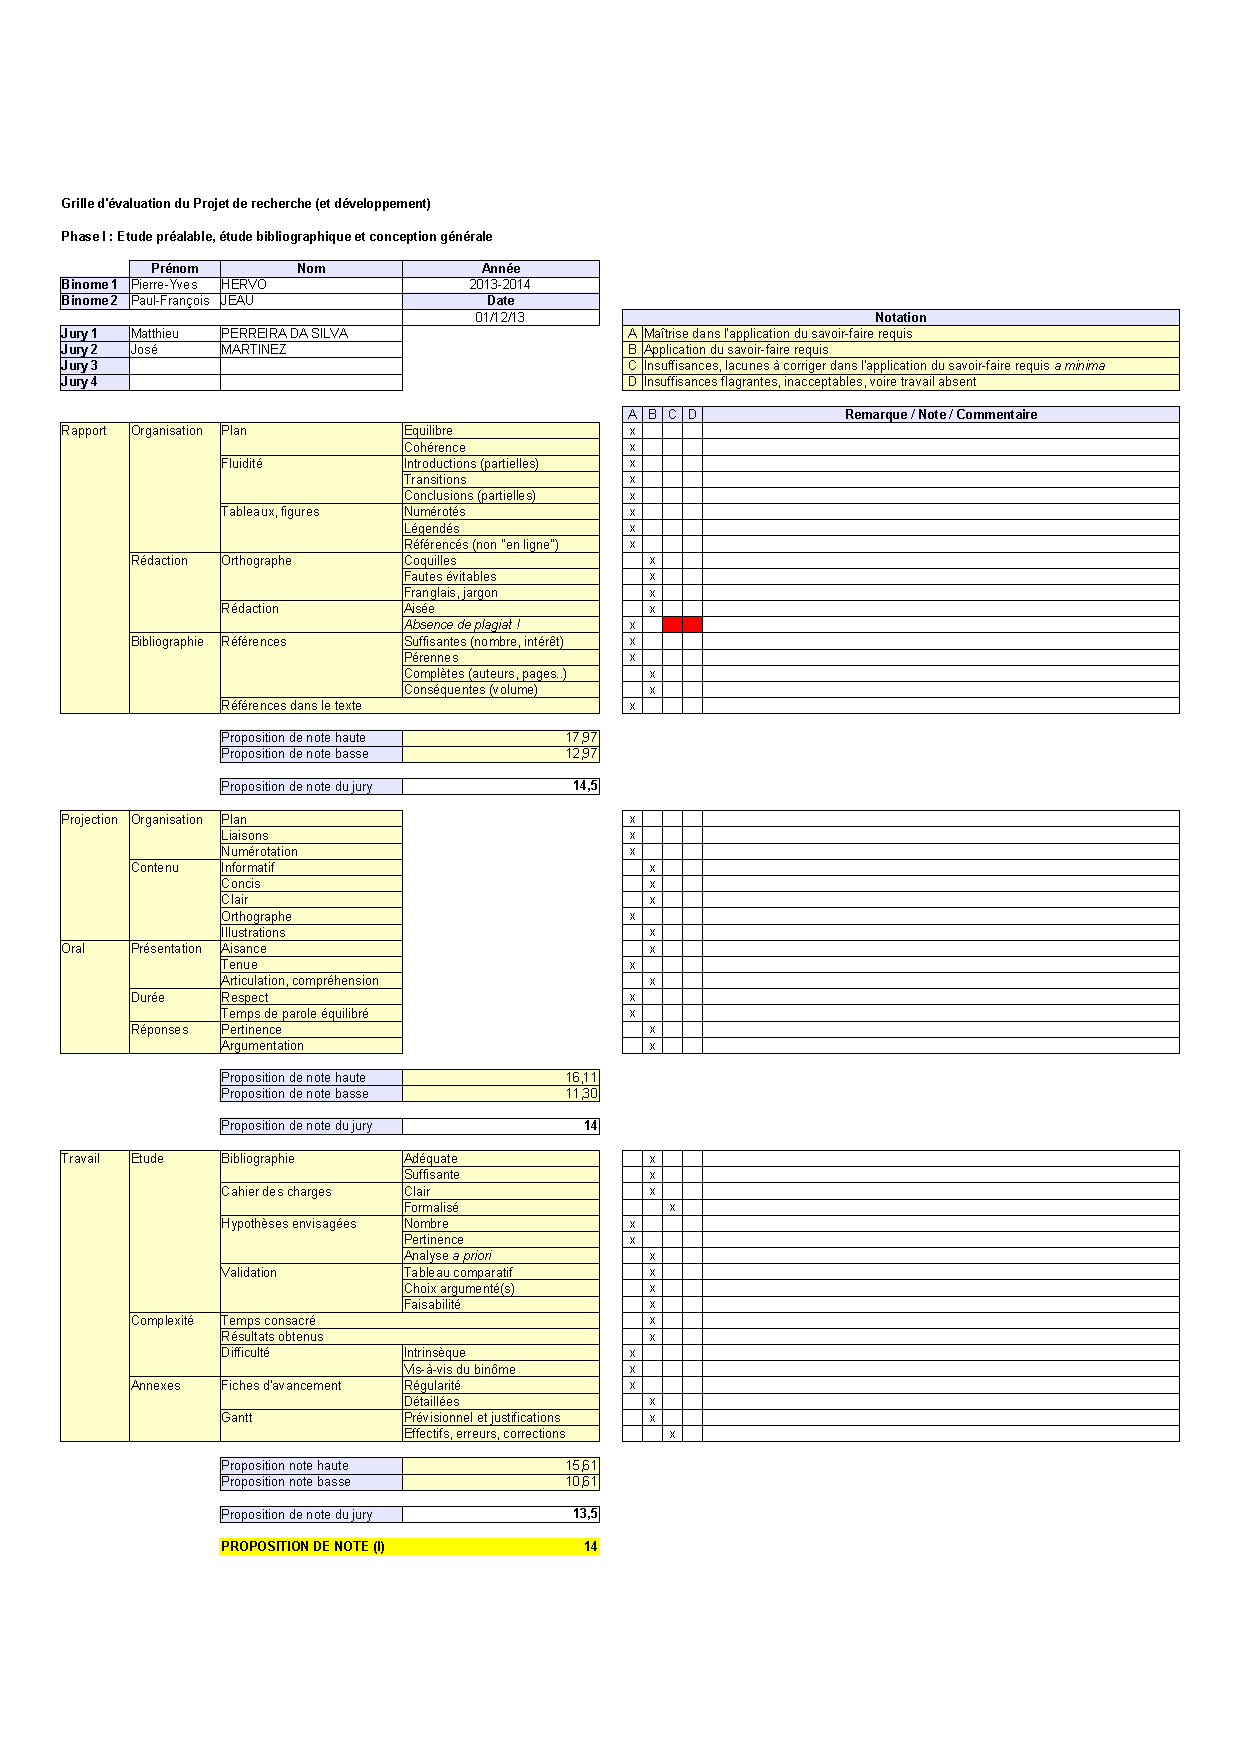
\includegraphics[width=0.9\textheight]{Images/Grille-Evaluation-PRD1}}
     \else
        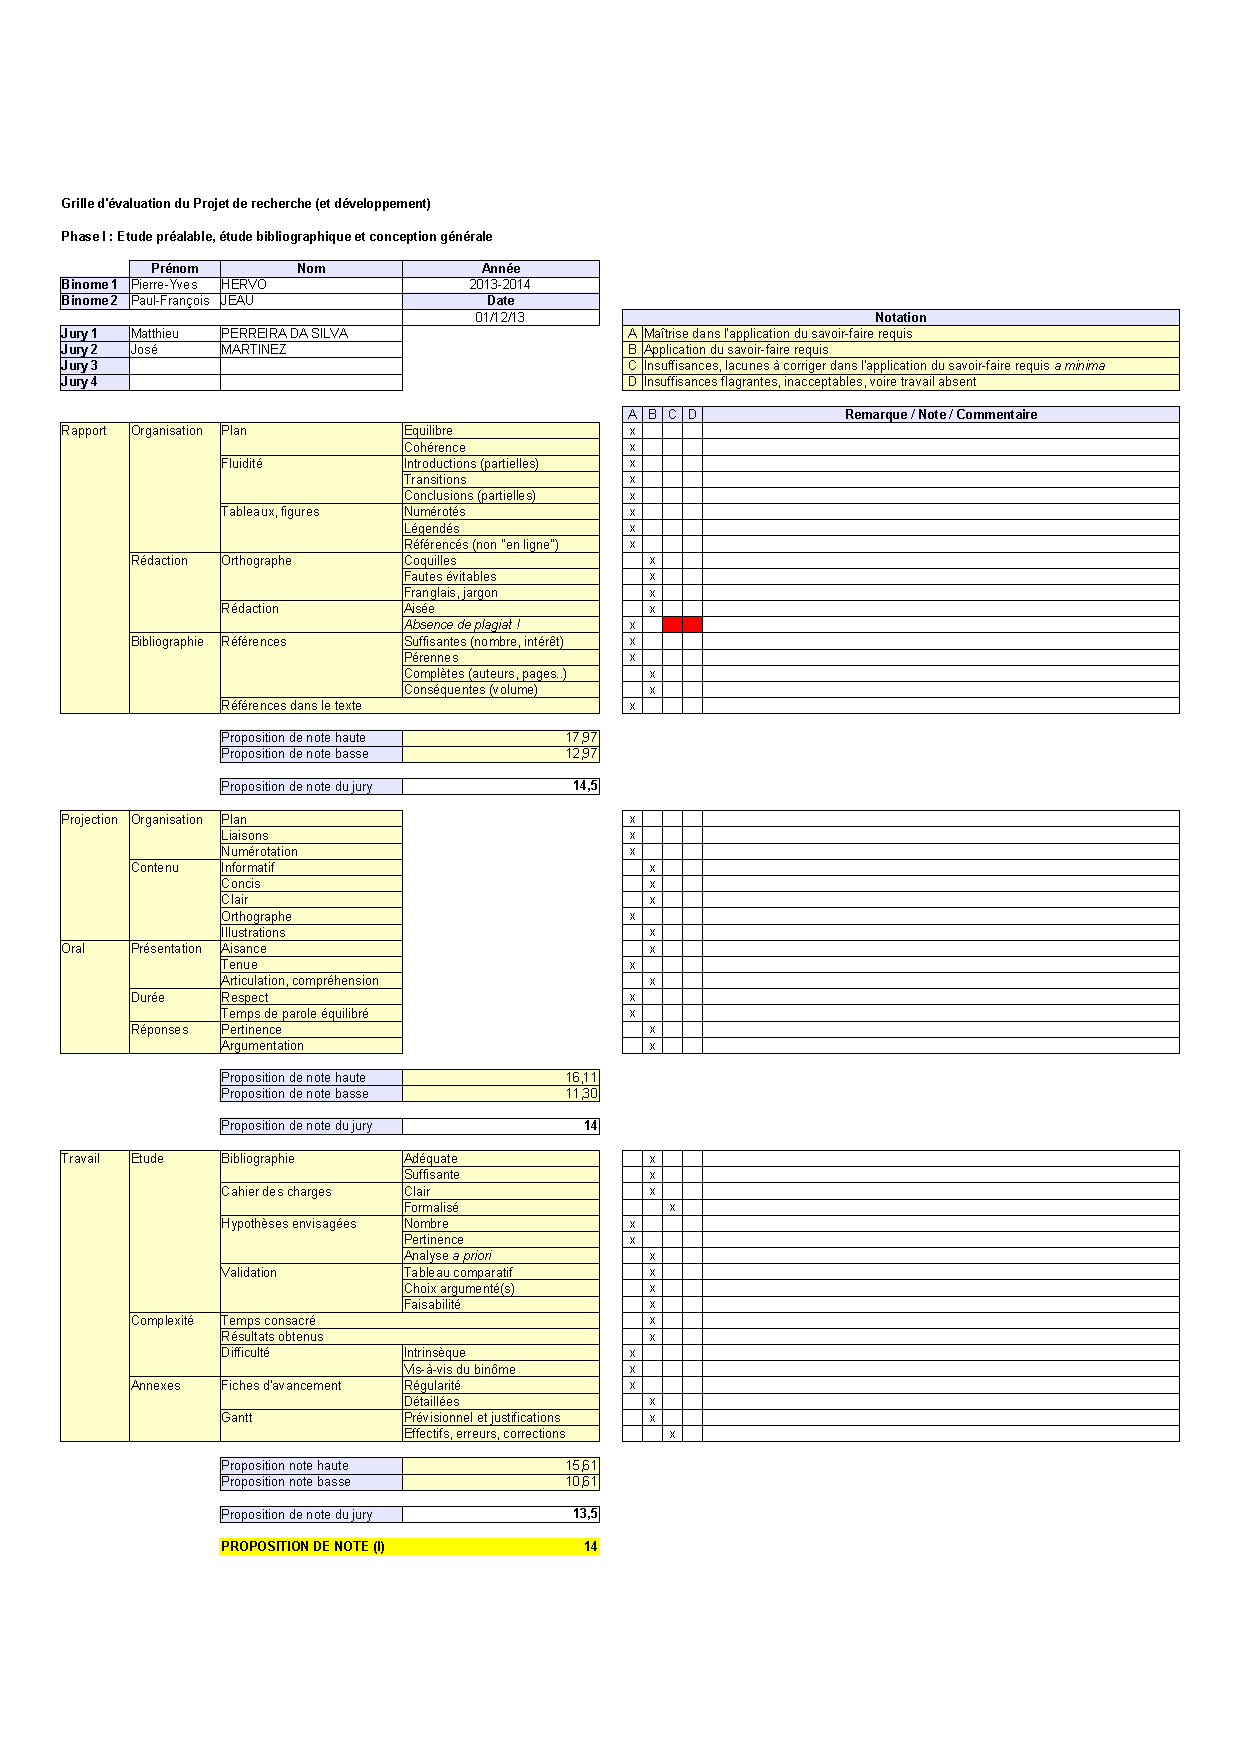
\includegraphics[width=0.9\textwidth]{Images/Grille-Evaluation-PRD1}
     \fi
	\caption{Points à contrôler à l'issue de la phase I}
	\label{fig:AutoEvaluationTravailIntermediaire}
\end{figure*}


\begin{figure*}
	\centering
     \ifscreen % macro TeX (issue de la classe report-rd-info.cls) permettant d'ajuster le contenu en fonction du l'orientation du document (<< screen >> ou pas)
        \rotatebox{90}{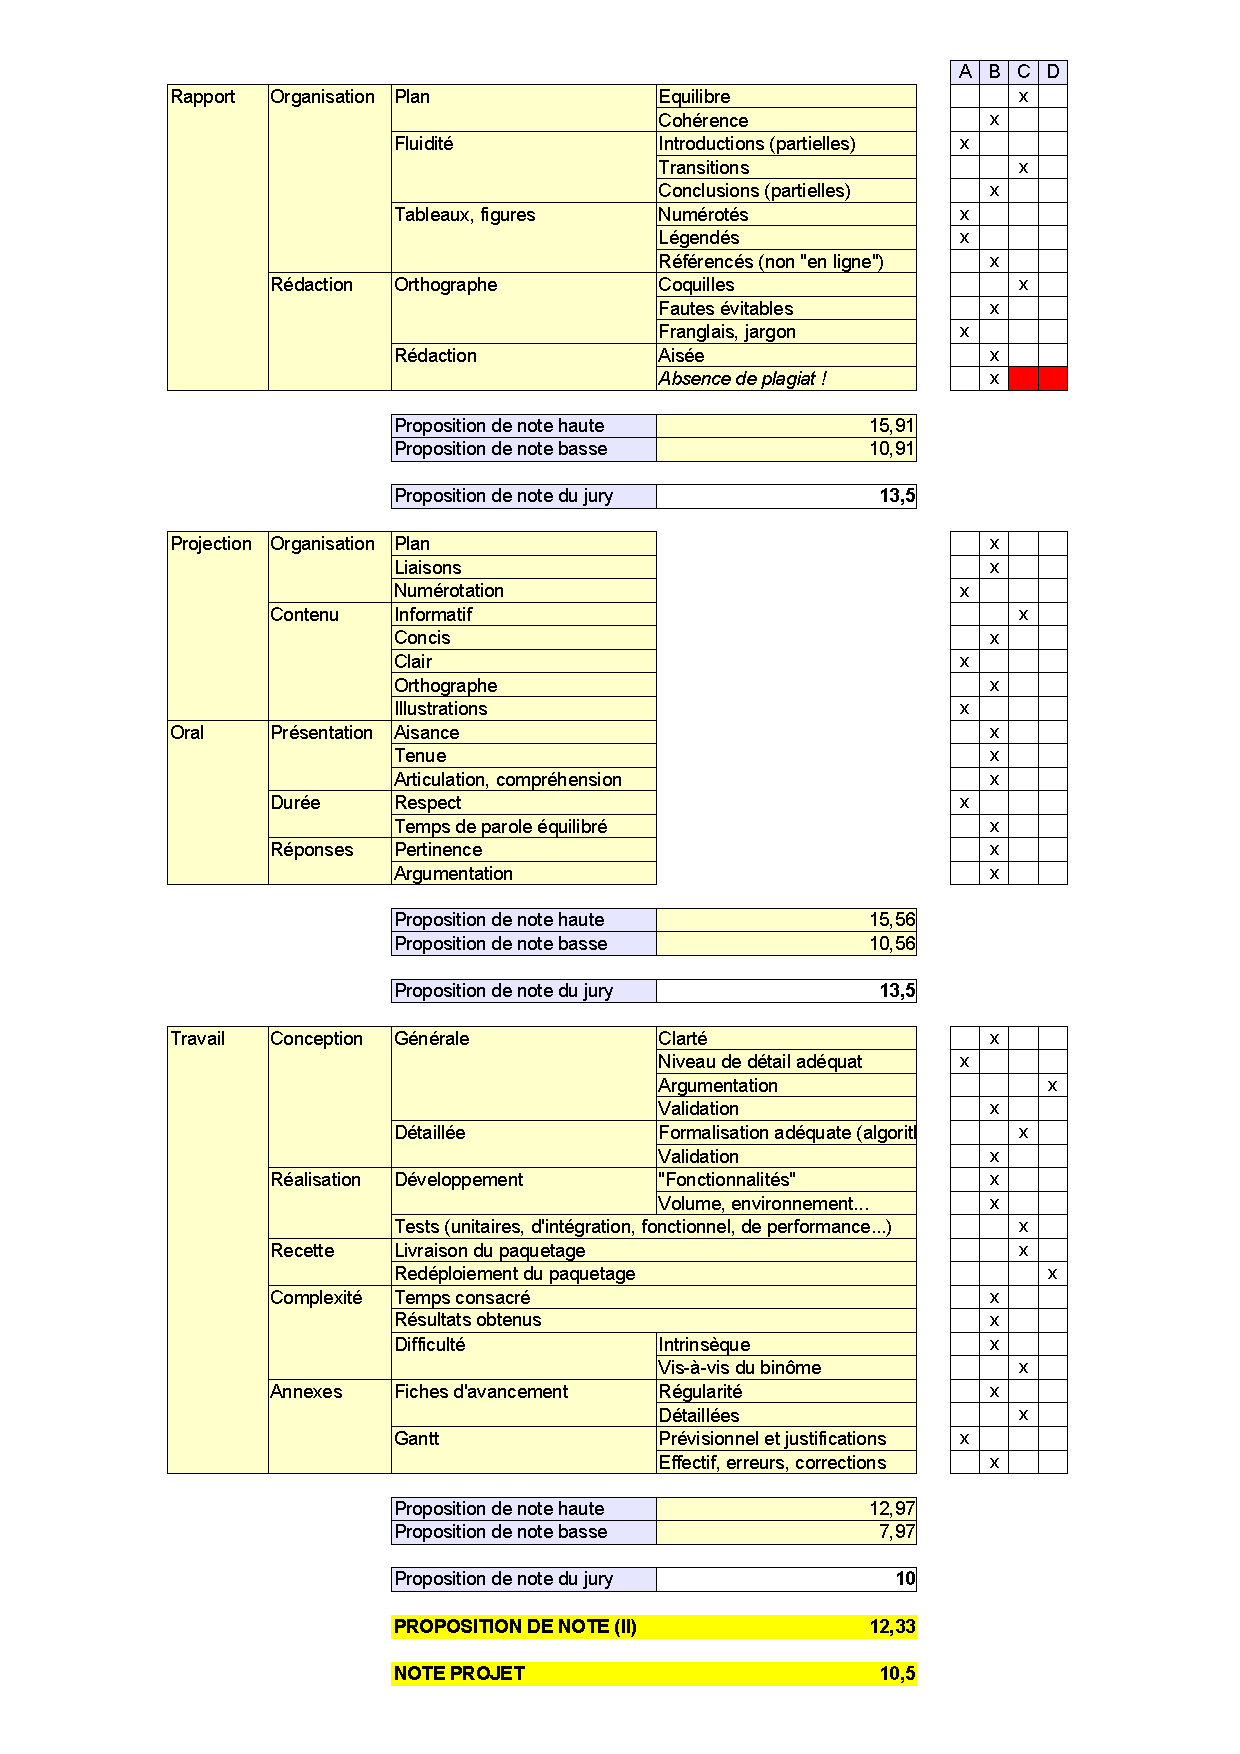
\includegraphics[width=0.9\textheight]{Images/Grille-Evaluation-PRD2}}
     \else
        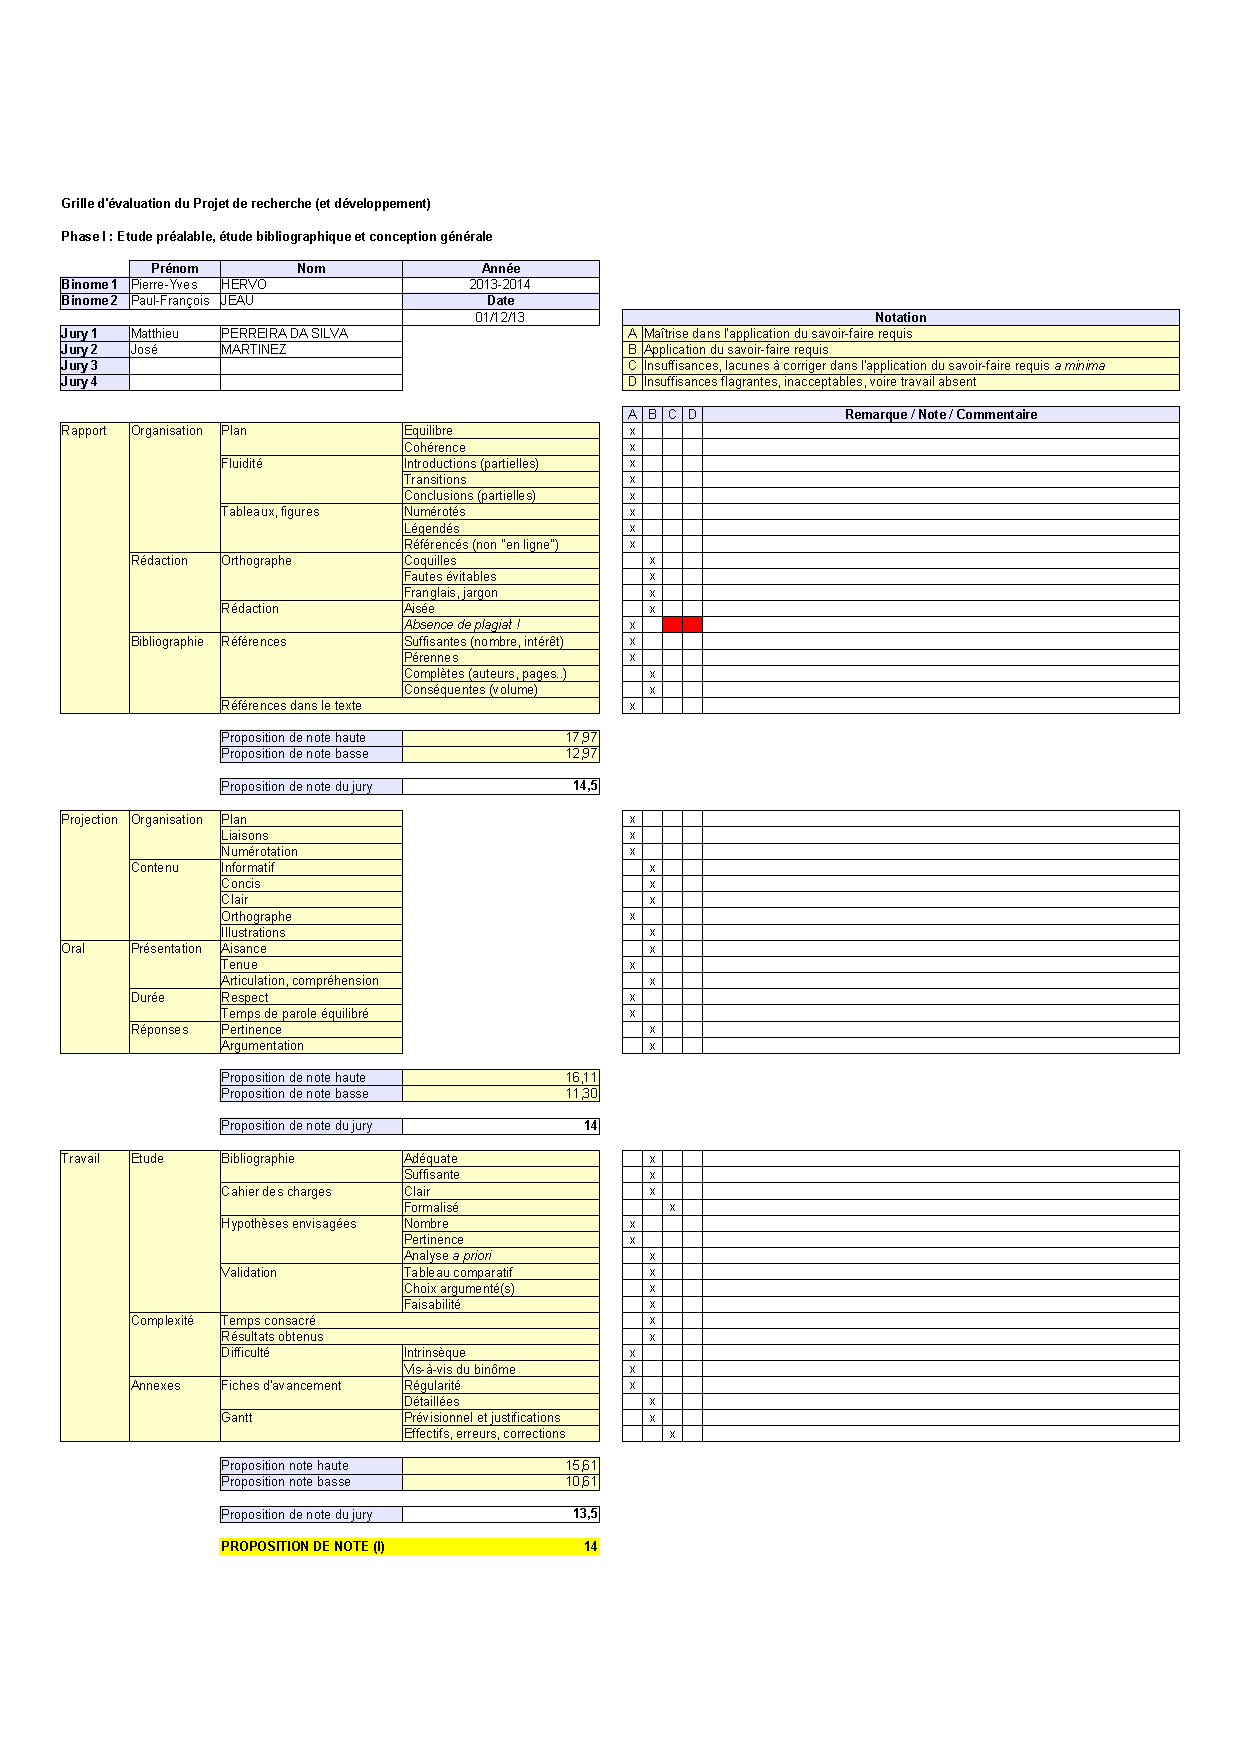
\includegraphics[width=0.9\textwidth]{Images/Grille-Evaluation-PRD1}
     \fi
	\caption{Points à contrôler à l'issue de la phase II}
	\label{fig:AutoEvaluationTravailFinal}
\end{figure*}


\end{document}

